
\begin{refsection}
\startcontents[chapters]	
\chapter{Stochastic Process}\label{ch:theory-of-stochastic-process}
\minitoc
	
\printcontents[chapters]{}{1}{}

\section{Stochastic process}\index{stochastic process}

\subsection{Basic definition and concepts}
\begin{definition}[stochastic process]\cite{dineen2013probability}
A stochastic process $X$ is a collection of random variables $\{X_t\}_{t\in T}$ on some fixed probability triple $(\Omega,\mathcal{F},P)$, indexed by a subset $T$ of the real numbers. 

If the index set is the positive integers, we call $X$ a \textbf{discrete-time stochastic process}. If the $T$ is an open interval on $\R$, it is called a \textbf{continuous-time stochastic process}

\end{definition}



\begin{definition}[sample path]\index{sample path}
\cite[45]{brzezniak1999basic} For a discrete-time stochastic process, the sequence of numbers $X_1(\omega),X_2(\omega),...$ for any fixed $\omega \in \Omega$ is called a sample path. For continuous stochastic process, the mapping $$t\in T \rightarrow X_t(\omega) \in \R$$
is a sample path. 
\end{definition}

\begin{remark}[interpretation]
	A stochastic process involves two variables, $t\in T,\omega \in \Omega$. For each fixed $t$, the mapping
	$$\omega \in \Omega \rightarrow X_t(\omega) \in \R$$
	is a random variable, and for each fixed $\omega$, the mapping $$t\in T \rightarrow X_t(\omega) \in \R$$
	is a sample path. 
\end{remark}

\begin{remark}[sample path examples]\hfill
\begin{itemize}
    \item One trivial case is that $X_1,X_2,...$ are the same mapping from sample space, then the sample path associated with a $\omega$ will be a horizontal line. However, if $X_1,X_2$ are different mapping from the sample space, then the sample path will not be a horizontal line. 
    \item For a non-trivial case: consider $X_t(\omega) = Z(\omega)\sin(t)$. If $Z(\omega)=0.5$, then $X_t = 0.5\sin(t)$
    \item For another non-trivial case: consider $X_t(\omega) = \omega^t$ assuming $\Omega=[0,1]$
\end{itemize}
\end{remark}

\begin{note}[interpretation on sample space and $\sigma$ algebra]\cite[97]{shreve2004stochastic2}\label{ch:theory-of-stochastic-process:remark:interpretationonsamplespaceandsigmaalgebra}\hfill
	Use random walk as example.
	\begin{itemize}
		\item Let $\omega \in \Omega$. One way to think of $\omega$ is as the random sample path. A random experiment is performed, and its outcome is the path of the random walk of horizon $T$. This random experiment outcome can be thought as a long sequence coin-toss outcome such that we map this long sequence coin-toss outcome to a random walk path, a function parameterized by time. See \autoref{ch:theory-of-stochastic-process:fig:randomWalkPaths}.
		\item If time index is from 0 to $T$, then total number of sample points in $\Omega$ is $2^T$.
		\item Some example random events in $\Omega$ are: (1) coin-toss sequences starting with H; (2) coin-toss sequence starting with HT.
		\item Then the $\sigma$-algebra is the $\sigma$-algebra on the sample-path space such that some 'suitable' subsets of all possible paths can be evaluated. For example, we can evaluate $P(W_t < 0.5)$ for some $t\geq 0$.
	\end{itemize}
\end{note}


\begin{figure}[H]
\centering
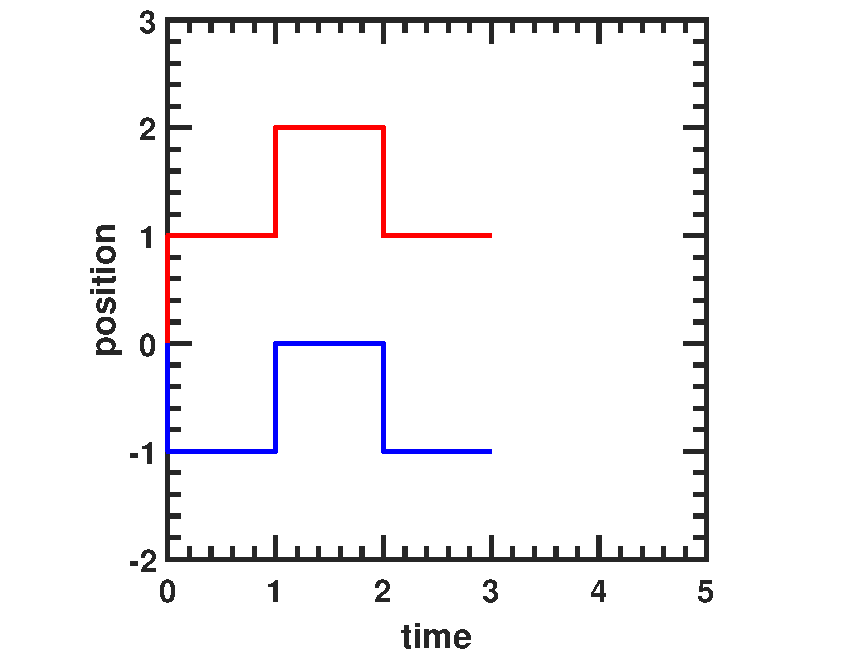
\includegraphics[width=0.7\linewidth]{figures/stochasticProcess/stochasticProcess/randomWalkPaths}
\caption{An illustration of a random walk mapping a sample point, $\omega$, to a trajectory parameterized by time, where red trajectory sample point HHT, and blue trajectory has sample point THT.}
\label{ch:theory-of-stochastic-process:fig:randomWalkPaths}
\end{figure}




\subsection{Filtration and adapted process}
\begin{definition}[filtration]
The collection $\{\cF_t,t\geq 0\}$ of $\sigma$-field on sample space $\Omega$ is called a filtration if
$$\cF_s \subseteq \cF_t,\forall 0 \leq s \leq t.$$
\end{definition}

\begin{remark}
	A filtration represents an increasing stream of information.
\end{remark}

\begin{definition}[adapted process]\index{adapted process}
\cite[77]{mikosch1998elementary}Consider a stochastic process $\{X_t\}_{t\in I}$ with a filtration $\{\cF_t\}_{t\in I}$ on its $\sigma$ field. The process is said to be \textbf{adapted to the filtration $\{\cF_t\}_{t\in I}$} if the random variable $X_t$ is $\cF_t$ measurable for all $t\in I$, or equivalently, $\sigma(X_t) \subseteq \cF_t$.
\end{definition}

\begin{remark}\cite{williams1991probability}\hfill
\begin{itemize}
    \item Examples of 'non-adapted' process. Consider a stochastic process $X$ with $I=\{0,1\}$. Let $\cF_0,\cF_1$ be $\sigma$ field generated by $X_0,X_1$. And $\cF_0$ and $\cF_1$ are independent to each other, i.e. $\cF_0 \nsubseteq \cF_1$.
    \item For a discrete stochastic process $\{X_n\}$, let $F_n = \sigma(X_0,X_1,...,X_n)$, then $\{X_n\}$ is an adapated process. Here $\sigma(X_0,X_1,...,X_n)$ is the smallest $\sigma$ algebra on $\Omega$ such that $X_0,X_1,...,X_n$ is measurable.
\end{itemize}
\end{remark}


\begin{remark}
	
\end{remark}

\subsection{Natural filtration of a stochastic process}\index{natural filtration}
\begin{definition}[natural filtration generated by a stochastic process]\label{ch:theory-of-stochastic-process:def:NaturalFiltrationGeneratedByStochasticProcesses}
Let $(S,\Sigma)$ be a measurable space. Let $X_t$ be a stochastic process such that $X:I\times\Omega \rightarrow S$, then natural filtration of $\cF$ with respect to $X$ is the filtration $\{\cF_t\}_{t\in I}$ given by
$$\cF_t = \sigma(X^{-1}_t(A)|s\in I,s \leq t, A \in \Sigma)$$
here $\sigma$ is the $\sigma$ field generation operation.
Or equivalently, we write
$$\cF_t = \sigma(X_s,s\leq t).$$	
\end{definition}

\begin{remark}\hfill
	\begin{itemize}
		\item In discrete setting, we have $\cF_n = \sigma(X_0,X_1,...,X_n)$.
		\item \textbf{Any stochastic process $X_t$ is an adapted process with respect to its natural filtration $\cF_t$ because $\sigma(X_t)\subseteq \cF_t$}.
	\end{itemize}
\end{remark}

\begin{remark}[interprete natural filtration]\cite[43]{bjork2009arbitrage}\hfill
\begin{itemize}
	\item Let the symbol $\cF_t^X$ denotes the $\sigma$-algebra (i.e., information) generated by $X_t$ on the interval $[0, t]$, or alternatively 'what has happened to X over the interval $[0, t]$'. Note that $\cF_t^X$ is one element in the natural filtration.
	\item (\textbf{interpretation of adaptivity}) Informally, if, based upon observations of the trajectory $\{X(s); 0 \leq s \leq t\}$, it is possible to decide whether a given \textbf{event} $A$ has occurred or not, then we write this as $\sigma(A) \in F^X_t$, or say that '$A$ is $F_t^X$-measurable'. 
	\item If the value of a given \textbf{random variable} $Z$ can be completely determined by given observations of the trajectory $\{X(s); 0 \leq s \leq t\}$, then we also write $\sigma(Z) \in F_t^X.$
	\item If $Y_t$ is a stochastic process such that we have $\sigma(Y(t))\in \cF_t^X, \forall t \geq 0$, then we say that $Y$ is adapted to the filtration $\{\cF_t^X, t\geq 0\}$.
\end{itemize}	

We have the following simple examples:
\begin{itemize}
	\item If we define the event $A$ by $A = \{X(s) \leq 3.14,\forall s\leq 9\}$, then we have $A\in \cF_9^X$.
	\item For the event $A=\{X(10) >8\}$, we have $A\in \cF_{10}^X$ but not $A\notin \cF_9^X$ since it is impossible to decide $A$ has occured or not based on the trajectory of $X_t$ over the interval $[0,9]$.
	\item For the random variable $Z$ defined by
	$$Z = \int_0^5 X(s)ds,$$
	we have $\sigma(Z)\in \cF_5^X.$
\end{itemize}
\end{remark}



\begin{example}[Trivial adaptive process: single Bernoulli experiment]
Consider a stochastic process $\{X_n\}$ represents a single toss experiment. We then have a trivial adapted process by defining $\cF_1 =\cF_2 =...=\cF_n = \cF = \sigma(X_1)$. For this filtration, the stochastic process $Z_n=\sum_{i=1}^n X_i$ is not adapted to it.	
\end{example}

\begin{example}[Infinite coin toss process(infinite Bernoulli experiments)]
Consider the probability space for tossing a coin infinitely many time. We can define the sample space as $\Omega_\infty = \text{the set of infinite sequences of Hs and Ts}$. A generic element of $\Omega_\infty$ will be denoted as $\omega=\omega_1\omega_2....$, where $\omega_n$ indicates the result of the $n$th coin toss.

We can define a stochastic process $\{X_n\}, X_n=f(W_1,W_2,...,W_n)$, and its filtration $\cF_n=\sigma(W_1,W2,...,W_n)$. Then every $X_n$ is $\cF_n$ measurable. A simple event in $\cF_n$ is the random experiment value of $W_1,W_2,...,W_n$. Note that as $n$ increase, $\cF_n$ becomes finer and finer, and $\cF_n$ can measure any previous $X_m,m<n$.	
\end{example}


\begin{remark}[$\sigma$ algebra for a stochastic process]
From \autoref{ch:theory-of-stochastic-process:remark:interpretationonsamplespaceandsigmaalgebra}, we know that $\cF$ is the $\sigma$ algebra for the set of all possible sample paths. And $\cF_t$ can be viewed as the $\sigma$ algebra for the set of all possible sample paths upto $t$. 	
	
\end{remark}


\subsection{Continuity of sample path}
\begin{definition}[continuity of sample path]
	A stochastic process with almost all sample paths continuous is called a continuous process. Similarly, a stochastic process is said to be right-continuous if almost all of its sample paths are right-continuous functions.
\end{definition}

\begin{example}\hfill
	\begin{itemize}
		\item The Brownian motion is a stochastic process with continuous sample path.
		\item The white noise process has discontinuous sample path. 
		\item The Poisson process has discontinuous sample path.
	\end{itemize}
\end{example}

\begin{definition}[right-continuous with left limit, cadlag]\hfill
	\begin{itemize}
		\item A sample path $X_t: [0,\infty) \to \R$ is called a right-continuous with left limit if for every $t\in [0,\infty)$ if
		\begin{itemize}
			\item the left limit $\lim_{s\to t^-} X(s)$ exists;
			\item the right limit $\lim_{s\to t^+ }X(s)$ exists and $\lim_{s\to t^+ }X(s) = f(t)$.
		\end{itemize}
		\item A stochastic process with almost all sample paths being right-continuous with left limit is called a cadlag stochastic process.
	\end{itemize}
\end{definition}

\begin{example}
	The sample path of a Poisson process is cadlag.	
\end{example}

\subsection{Predictable process}

\begin{definition}[predictable process]\index{predictable process}\index{previsible process}\hfill
\begin{itemize}
	\item Given a probability space $(\Omega, \cF, P)$ and a filtration $\{\cF_n\}_{n\in \N}$, a discrete-time stochastic process $\{X_n\}_{n\in \N}$ is \textbf{predictable} if $X_{n+1}$ is measurable with respect to $\cF_n$ for each $n$.
	\item  Consider a probability space $(\Omega, \cF, P)$ and a filtration $\{\cF_t\}_{t\geq 0}$. Let $\cP$ denote the predictable/previsible $\sigma$-algebra, i.e. the $\sigma$-algebra generated by all left-continuous process adapted to $\{\cF_t\}_{t\geq 0}$. If a process $X_{t}$ is measurable with respect to $\cP$ for all $t$, then $X_t$ is a predictable process.
\end{itemize}	
\end{definition}


\begin{figure}[H]
	\centering
	\begin{subfigure}[b]{0.4\textwidth}
		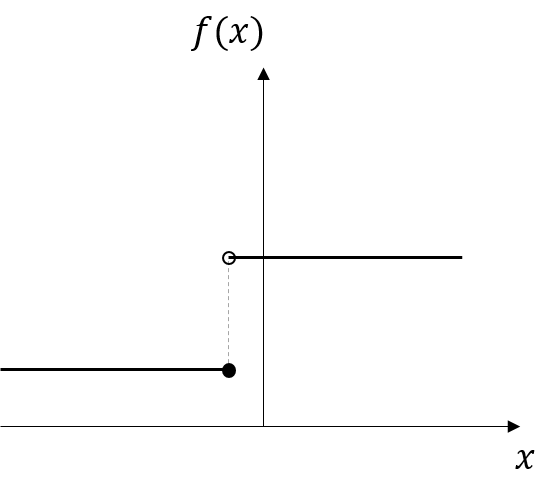
\includegraphics[width=\textwidth]{figures/mathFundamentals/LeftContinuousFunctionDemo}
		\caption{A left continuous function.}
	\end{subfigure}\quad
	\begin{subfigure}[b]{0.4\textwidth}
		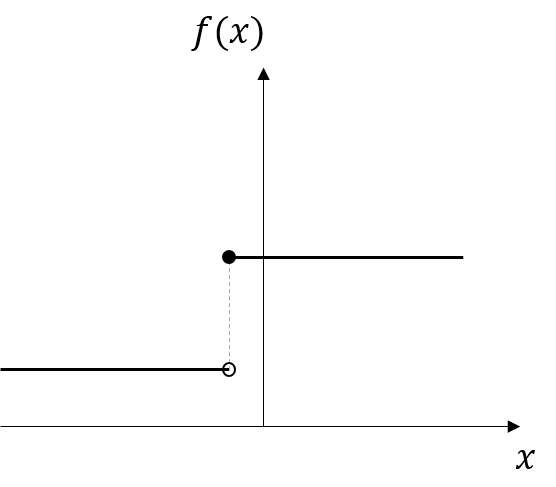
\includegraphics[width=\textwidth]{figures/mathFundamentals/RightContinuousFunctionDemo}
		\caption{A right continuous function.}
	\end{subfigure}
	\caption{An illustration of left and right continuous functions.}
\end{figure}

\begin{example}\hfill
\begin{itemize}
	\item Every deterministic process is a predictable process.
	\item Every continuous-time stochasti process with continuous smaple path (e.g., Brownian motion) is adapted to and predictable with respect to its natrual filtration.
\end{itemize}	
\end{example}


\begin{example}[trading strategies as predictable processes]
\end{example}


\section{Stationary process}
\subsection{Stationarity concepts}
\begin{definition}[strictly stationary process]\index{strictly stationary process}\cite[231]{koralov2007theory}\cite[30]{lindgren2013stationary}
	A random process $\{X_t\}_{t\in T}$ over probability space $(\R, \cB(\R), P)$ is called strictly stationary if for any $t_1,t_2,...,t_k\in T$ and $A_1,...,A_k \in \cB(\R)$
	the probabilities
	$$P(X_{t_1 + t}\in A_1,...,X_{t_k + t}\in A_k)$$
	do not depend on arbitrary $t$, where $t\in T$.
\end{definition}

\begin{example}[a sequence of iid random variables]
	A sequence of independent identically distributed random variables is a strictly stationary process.
\end{example}

\begin{lemma}[A Markov chain starting from stationary distribution is strictly stationary process]\cite[231]{koralov2007theory}
	Consider a finite state, irreducible and aperiodic Markov chain characterized by matrix $P$. Let the initial state distribution be $\pi_0$. If the stationary distribution $\pi = \pi_0$, then the Markov chain $P$ is a strictly stationary process.
\end{lemma}
\begin{proof}
	The stationary distribution will exist(\autoref{ch:markov-chains:th:basiclimittheoremmarkovchain}). By iteration, we know that the distribution at every time step is $\pi$. 
\end{proof}




\begin{definition}[weakly stationary process]\index{weakly stationary process}\cite[209]{koralov2007theory}\cite[32]{lindgren2013stationary}
	A random process $\{X_t\}_{t\in T}$ is called a weakly stationary process if there exist a constant $m$ and $b(t),t\in T$ function, such that
	$$E[X_t] = m, Var[X_{t_1}] = \sigma^2 ,cov(X_{t_1},X_{t_2}) = r(t_1 - t_2),\forall t_1\neq t_2 \in T,$$
	where $b(0) = \sigma^2.$ 
	
	That is, the mean and the covariance structure a weakly stationary process can be fully characterized by a constant mean parameter and a covariance function $r: \R\to \R$.
\end{definition}


\begin{lemma}[properties of a covariance function]\cite[35]{lindgren2013stationary}
	For a weakly stationary stochastic process, the covariance function $r(t_1-t_2) \triangleq Cov(X(t_1),X(t_2))$ has the following properties:
	\begin{itemize}
		\item $r(0) = Var[X(t)] \geq 0,\forall t$
		\item $Var[X(t+h)\pm X(t)] = E[(X(t+h)\pm X(t))^2] = 2(r(0)\pm r(h))$
		\item (even function)$r(\tau) = r(-\tau)$.
		\item $\abs{r(\tau)} \leq r(0)$.
		\item If $\abs{r(\tau)}= r(0)$, for some $\tau \neq 0$, then $r$ is periodic. In particular,
		\begin{itemize}
			\item If $r(\tau) = r(0)$, then $X(t+\tau) = X(t), \forall t$.
			\item If $r(\tau) = -r(0)$, then $X(t+\tau) = -X(t) = X(t-\tau), \forall t$(periodicity of $2\pi$).
		\end{itemize}
		\item If $r(\tau)$ is continuous for $\tau = 0$, then $r(\tau)$ is continuous everywhere.  
	\end{itemize}	
\end{lemma}
\begin{proof}
	(1)(2)(3) Straight forward.
	
	(4) Use Cauchy inequality for random variables(\autoref{ch:theory-of-probability:th:Cauchy-SchwarzInequality})
	$$E[\abs{X(t) - \mu}\abs{X(t+\tau) - \mu}] \leq \sqrt{Var[X(t)]Var[X(t+\tau)]} = \sqrt{r(0)^2} = r(0).$$
	(5)
	
	(a) If $r(\tau)=r(0)$, then from (2) we have $E[(X(t+\tau)-X(t))^2] = 0$. It can be showed via contradiction that having $E[(X(t+\tau)-X(t))^2] = 0$ implies $X(t+\tau) = X(t)$(that is the two maps are exactly the same).
	(b) If $r(\tau)=-r(0)$, then from (2) we have $E[(X(t+\tau)+X(t))^2] = 0$. It can be showed via contradiction that having $E[(X(t+\tau)+X(t))^2] = 0$ implies $X(t+\tau) = -X(t)$(that is the two maps are exactly the same). 
	(6) For any $t$, consider
	\begin{align*}
	(r(t+h) - r(t))^2 &= (Cov(X(0),X(t+h)) - Cov(X(0),X(t)))^2 \\
	&= (Cov(X(0),X(t+h) - X(t)))^2 \\
	&\leq Var[X(0)]Var[X(t+h) - X(t)] = 2r(0)(r(0) - r(h))
	\end{align*}
	If $h\to 0$, then $r(0) - r(h)\to 0^+$ due to the continuity of $r(\tau)$ at $\tau(0)$,which implies $r(t+h)\to r(t)$(that is, $r(t)$ is continuous for any $t$).
\end{proof}

\begin{lemma}[a strictly stationary process is a weakly stationary process]
	A strictly stationary process $X_t$ will be a weakly stationary process.
\end{lemma}
\begin{proof}
	For mean, use translation invariant property of of marginal distribution. For covariance, use translational invariant property of two variable joint distribution.
\end{proof}


\begin{lemma}\label{ch:theory-of-stochastic-process:weaklystationaryGaussianisstationary}A weakly stationary Gaussian process is a strictly stationary Gaussian process.
\end{lemma}
\begin{proof}
	To a process is strictly stationary, we need to show $(X_{t_1+\tau},X_{t_2+\tau},...,X_{t_n+\tau}),\forall \tau \in \R$ has the same distribution as 	$(X_{t_1+\tau},X_{t_2+\tau},...,X_{t_n+\tau})$. Because the full distribution of a multivariate Gaussian can be constructed from its pair distribution(\autoref{ch:theory-of-statistics:th:MultivariateGaussainFulldistributionFromPairdistribution}), we only need to show that $(X_{t_1+\tau},X_{t_2+\tau}),\tau \in \R$ has the same distribution as $(X_{t_1},X_{t_2})$. From weak stationarity, we know that the mean vector and covariance matrix are the same; that is, their joint distribution are the same.
	Note that for a Gaussian distribution, mean and covaraince matrix fully determines the joint distribution.
\end{proof}



\subsection{Random phase and amplitude}
\begin{definition}[random harmonic function]\index{random harmonic function}\cite[35]{lindgren2013stationary}
	Let $A > 0$ and $\phi$ be independent random variable, with $\phi$ uniform over $[0,2\pi]$. The stochastic process $X(t)$ defined by
	$$X(t) = A \cos(2\pi f_0 t + \phi).$$	
\end{definition}



\begin{lemma}[random harmonic function]\cite[36]{lindgren2013stationary}
	The random harmonic function $X(t) = A\cos(2\pi f_0 t + \phi)$ is a \textbf{stationary process} if $A$ and $\phi$ are independent and $\phi$ is uniformly distributed in $[0,2\pi]$. Then
	\begin{itemize}
		\item $E[X(t)] = 0$
		\item $Var[X(t)] = \frac{1}{2}E[A^2] = \sigma^2$
		\item $r(\tau) = \sigma^2 \cos (2\pi f_0 \tau)$ 
	\end{itemize}	
\end{lemma}
\begin{proof}
	(1) $$E[X(t)] = E[A\cos(2\pi f_0 t + \phi)] =  E[A]E[\cos(2\pi f_0 t + \phi)]$$
	\begin{align*}
	E[\cos(2\pi f_0 t + \phi)] & = \int_0^{2\pi} \cos(2\pi f_0 t + x)\frac{1}{2\pi}dx \\
	&=\frac{1}{2\pi}(\sin(2\pi f_0 t + 2\pi) - \sin(2\pi f_0 t + x)) \\
	&= 0.
	\end{align*}	
	(2) $$Var[X(t)] = E[X(t)^2] = E[A^2\cos(2\pi f_0 t + \phi)^2] = E[A^2]E[\cos(2\pi f_0 t + \phi)^2].$$
	Note that
	\begin{align*}
	E[\cos(2\pi f_0 t + \phi)^2] & = \int_0^{2\pi} \cos(2\pi f_0 t + x)^2\frac{1}{2\pi}dx \\
	&=\frac{1}{2\pi}(\pi) \\
	&= 1/2.
	\end{align*}
	(3) $$Cov(X(t),X(s)) = E[X(t)X(s)] = E[A^2]E[\cos(2\pi f_0 t + \phi)\cos(2\pi f_0 s + \phi)].$$
	Note that
	\begin{align*}
	E[\cos(2\pi f_0 t + \phi)\cos(2\pi f_0 s + \phi)] & = \frac{1}{2\pi}\int_0^{2\pi} \frac{1}{2}(\cos(2\pi f_0 (s + t) + 2x) + \cos(2\pi f_0(s - t)) )dx \\
	&=\frac{1}{2} \cos(2\pi f_0(s - t))
	\end{align*}
\end{proof}



\begin{lemma}[linear supposition of random harmonic function]\cite[38]{lindgren2013stationary}
	The linear supposition of random harmonic functions	
	$$X(t) = A_0 + \sum_{k=1}^n A_k \cos(2\pi f_k t + \phi_k)$$
	with deterministic constants $A_0, A_1,...,A_k$ and independent uniform random variables $\phi_1,\phi_2,...,\phi_k$ has the following properties:
	\begin{itemize}
		\item $E[X(t)] = A_0.$
		\item $r(\tau) = \sigma_0^2 + \sum_{k=1}^n \sigma_k^2 \cos (2\pi f_k \tau)$.
	\end{itemize}	
\end{lemma}
\begin{proof}
	(1) 
	$$E[ A_0 + \sum_{k=1}^n A_k \cos(2\pi f_k t + \phi_k)] = E[A_0] + 0.$$
	(2)
	Note that
	\begin{align*}
	& E[\sum_{k=1}^n A_j \cos(2\pi f_k t + \phi_k) \sum_{k=1}^n A_k \cos(2\pi f_k (t+\tau) + \phi_k)] \\
	&= E[\sum_{j=1}^n A_j \cos(2\pi f_j t + \phi_j) \sum_{k=1}^n A_k \cos(2\pi f_k (t+\tau) + \phi_k)] \\
	&= \sum_{k=1}^n E[ A_k^2] E[ \cos(2\pi f_k t + \phi_k) \cos(2\pi f_k (t+\tau) + \phi_k)] \\
	&= \sum_{k=1}^n \sigma_k^2 \cos (2\pi f_k \tau)
	\end{align*}
\end{proof}




\begin{lemma}[power and average power]\cite[39]{lindgren2013stationary}
	Consider the linear supposition of random harmonic functions	
	$$X(t) = A_0 + \sum_{k=1}^n A_k \cos(2\pi f_k t + \phi_k)$$
	with deterministic constants $A_0, A_1,...,A_k$ and independent uniform random variables $\phi_1,\phi_2,...,\phi_k$.
	
	Then the average power is given by
	$$E_T = \lim_{T\to \infty} \frac{1}{T}\int_0^T X(t)^2 dt = A_0^2 + \frac{1}{2}\sum_{k=1}^n A_k^2.$$	
\end{lemma}
\begin{proof}
	Note that	
	\begin{align*}
	E_T &= \frac{1}{T}\int_0^T X(t)^2 dt \\
	&= \frac{1}{T}\{TA_0^2 + 2\sum_{k=1}^n A_0A_k\int_0^T \cos(2\pi f_k t + \phi_k) dt \\
	& + \sum_{k=1}^n A_k^2 \int_0^T \cos^2(2\pi f_k t + \phi_k)dt \\
	& + 2\sum_{k=1}^n\sum_{l = k+1}^n  A_kA_l \int_0^T \cos(2\pi f_k t + \phi_k)\cos(2\pi f_l t + \phi_l)dt 
	\}.
	\end{align*}
	
	Further note that:
	$$\lim_{T\to \infty} \frac{1}{T} \int_0^T \cos(2\pi f_k t + \phi_k) dt = 0$$
	since $\int_0^T \cos(2\pi f_k t + \phi_k) dt$ is bounded. 
	
	
	$$\lim_{T\to \infty} \frac{1}{T} \int_0^T \cos(2\pi f_k t + \phi_k)\cos(2\pi f_l t + \phi_l)dt = 0$$
	since $\int_0^T \cos(2\pi f_k t + \phi_k)\cos(2\pi f_l t + \phi_l)dt$ is bounded. 
	
	$$\lim_{T\to \infty} \frac{1}{T} \int_0^T \cos^2(2\pi f_k t + \phi_k)dt = \frac{1}{2}$$
	since $\int_0^T \cos^2(2\pi f_k t + \phi_k)dt = \frac{T}{2}$ is bounded. 
	
\end{proof}


\begin{remark}[average power is independent of sample path]
Note that the integral is independent of $\phi_1,...,\phi_k$. That is, no matter what values  $\phi_1,...,\phi_k$ are taking in a sample path, we get the same average power.	
\end{remark}


\subsection{Ergodicity}




\subsection{Spectral analysis}

\begin{definition}[spectral distribution, spectral density]
If a stationary stochastic process $X_t$ has autocovariance function $\gamma(\tau)$ satisfying $\int_{-\infty}^{\infty} \abs{\gamma(\tau)}d\tau$, then we define the \textbf{spectral density function} as
$$f(\omega) = \int_{-\infty}^{\infty} \gamma(\tau) \exp(-2\pi i \omega \tau) d\tau,$$
where $-\infty < \omega < \infty$.	
\end{definition}


\begin{lemma}[properties of spectral density function]\hfill
\begin{itemize}
	\item $f(\omega)$ is real-valued.
	\item $f(\omega) > 0$.
	\item $f(\omega)$ is even.
	\item $f(\omega)$ is periodic with period 1.
	\item $\gamma(\tau) = \int_{=1/2}^{1/2} f(\omega) \exp(2\pi i \omega \tau) d\omega$.
\end{itemize}	
\end{lemma}


\begin{theorem}[Wiener-Khintchine Theorem]
	
\end{theorem}


\subsection{Monte carlo simulation}


\section{Gaussian process and Finite dimension distributions}
\subsection{One-dimensional Gaussian process}
\subsubsection{Definitions and properties}
\begin{definition}[One-dimensional Gaussian process]\index{Gaussian process}
	A stochastic process $\{X_t\}_{t\in T}$ is Gaussian process if for any $t_1,t_2,...,t_n\in T$, the joint distribution on $(X_{t_1},...,X_{t_n})$ is Gaussian, i.e., $$p(x_1,x_2,...,x_n)=\frac{1}{(2\pi)^{n/2}}\frac{1}{\abs{det \Sigma}^{1/2}}\exp(-\frac{1}{2}(x-\mu)^T\Sigma^{-1}(x-\mu)).$$
\end{definition}

\begin{definition}[One-dimensional Gaussian process, alternative]\cite[19]{lindgren2012stationary}
	A stochastic process $\{X_t\}_{t\in T}$ is Gaussian process if every linear combination $$S = \sum_k a_k x(t_k),t_k\in T, a_k\in \R$$
	has a Gaussian distribution. 	
\end{definition}


\begin{remark}[equivalence of two definitions]\hfill
\begin{itemize}
	\item The first definition can imply the second by affine transformation \autoref{ch:theory-of-statistics:th:affinetransformmultivariatenormal}.
	\item The second can imply the first by using the multivariate Gaussian definition via linear combination(\autoref{ch:theory-of-statistics:th:MultivariateGaussianDefinitionViaLinearCombination}).
\end{itemize}	
\end{remark}

\begin{lemma}[affine transformation of a Gaussian process is a Gaussian process]
Let $X_t$ be a Gaussian process, then $aX_t + b, a, b\in \R$ is also a Gaussian process. 
\end{lemma}
\begin{proof}
Directly from definitions.
\end{proof}




\begin{note}[Gaussian processes can be stationary or non-stationary]
	A Gaussian process can be stationary(white noise process) or non-stationary(Wiener process).
\end{note}


\subsubsection{Stationarity}

\begin{lemma}
If $X(t)$ is a stationary Gaussian process with mean $m$ and covariance function $r(\tau)$.
Then
\begin{itemize}
	\item For all $t$, $X(t)\sim N(m, r(0)^2)$.
	\item For all $t_1,t_2$, $(X(t_1),X(t_2)) \sim MN(\mu, \Sigma)$,
	where
	$$\mu = \begin{bmatrix}
	m\\
	m
	\end{bmatrix}, \Sigma = \begin{bmatrix}
	r(0) & r(t_1 - t_2) \\
	r(t_1-t_2) & r(0) 
	\end{bmatrix}$$
\end{itemize}	
\end{lemma}
\begin{proof}
Straight forward.
\end{proof}


\subsubsection{Examples}

\begin{example}[white noise process]
A white noise process $W_t$ is a Gaussian process with zero mean and $cov(W_t,W_s) = \sigma^2\delta(s-t).$
\end{example}

\begin{example}[a discrete random walk is not a Gaussian process]
A random walk $B_n$ is not a Gaussian process. For example, $B_1$ is a Bernoulli distribution, not a Gaussian.
\end{example}

\begin{example}[Ornstein-Uhlenbeck process is stationary Gaussian process in the long run]
An OU process is a Gaussian process.
As $t\to \infty$, the OU process becomes a stationary Gaussian process(\autoref{ch:theory-of-stochastic-process:th:OUprocesssolution}).
\end{example}



\begin{example}[a Wiener process(Brownian motion) is a Gaussian process]
From \autoref{ch:theory-of-stochastic-process:th:Brownianmotionbasicproperty}, a Wiener process is the integral of a white noise Gaussian process. It is not stationary, but it has stationary increments.
\end{example}

\begin{example}[a geometric Brownian motion is not a Gaussian process]
Let $X_t$ be a geometric Brownian motion process, then $X_t$ is not Gaussian, thus not a Gaussian process.
\end{example}

\begin{example}[a stable AR(1) process]
A stable AR(1) process of $X_k$ can be written as
$$X_k = \sum_{i=0}^\infty \beta^i W_{k-i},$$
where $W_k = w(t_k)$ is the discrete sampling of wiener process $w(t)$.

Because any linear combination of samples of a Gaussian process $w(t)$ is a normal random variable, $X_k$	has a normal distribution.
\end{example}





\subsection{finite dimensional distribution}

\begin{definition}\index{finite dimensional distribution}
The finite dimensional distribution of a stochastic process $X$ is the joint distribution of $X_{t_1},X_{t_2},...,X_{t_k}$, where $t_1,t_2,...,t_k \in \mathcal{I}$, we represent the probability measure as
$$\mu_{t_1,t_2,...,t_k}(F_1\times F_2 \times ... F_k) = P(X_{t_1}\in F_1 ... X_{t_k}\in F_k)$$
where $F_i$ are measurable events/subsets in $\R$.
\end{definition}


\begin{remark}[purpose]
We usually characterize a stochastic process by studying the joint distribution of a finite set of random variables in the stochastic process. 	
\end{remark}


\begin{mdframed}
\textbf{consistence of finite-dimensional distributions}\\
Given a set of finite-dimensional distributions on different index set, to make sure that these fdd are derived from the same stochastic process, \textbf{we require these fdd to be consistent based on two criteria:}\cite[lec 4]{Holmes-Cerfon2015applied}
\begin{itemize}
    \item Invariant under permutations, i.e., two probability measure on two different set of $X_1,X_2,...,X_k$ and $X_{\pi(1)},..,X_{\pi(k)}$, then the measure should be the same given the same measurable subset.
    \item Marginal distribution are consistent,i.e., marginalizing different probability measure to the marginal measure to the same subset of random variables should be the same.
\end{itemize}
\end{mdframed}

\begin{theorem}[Kolmogorov Extension theorem] If the family of measures $\{\mu_{t_1,...,t_k}\}$ satisfies the consistent condition, then there exists a stochastic process with the corresponding finite-dimensional distribution.
\end{theorem}


\subsection{Gaussian process generated by Brownian motin}
\begin{lemma}[Gaussian process stochastic differential equation]\label{ch:theory-of-stochastic-process:th:GaussianprocessSDE}
	A stochastic process $X_t$ governed by 
	$$dX_t = a(t)dt + b(t)dW_t,$$
	where $W_t$ is a Wiener process, is a Gaussian process.
\end{lemma}
\begin{proof}
	It can be showed that $X(t) \sim N(\mu(t),\int_0^t b(s)^2ds)$(\autoref{ch:theory-of-stochastic-process:th:arithmeticSDE}). Also note that the increment is independent and Gaussian; that is $X(t_1)-X(t_2)$ is independent of $X(t_2)-X(t_3),t_1>t_2>t_3$. Therefore, the random vector $(X(t_1),X(t_2),...,X(t_n))$ is multivariate normal since it can be constructed by affine transformation of $(X(t_1)-X(t_2),X(t_2)-X(t_3),..., X(t_n)$(\autoref{ch:theory-of-statistics:th:affinetransformmultivariatenormal}).
\end{proof}


\begin{theorem}[linear combination of multiple Brownian-motion-generated Gaussian processes is a Gaussian process]\label{ch:theory-of-stochastic-process:th:linearCombinationOfBrownianMotionGeneratedGaussainProcess}
Consider $N$ stochastic processes generated by $M$ Brownian motions, given by
$$dX_i(t) = \mu_i(t) dt + \sum_{j=1}^M \sigma_{ij}(t) dW_j,$$
where $W_1,W_2,...,W_M$ are independent Brownian motion, $\mu_i(t), \sigma_{ij}(t)$ are state-independent deterministic function of $t$. 


Then 
\begin{itemize}
	\item the joint distribution of $X_1,X_2,...,X_N$ is multivariate Gaussian.
	\item for any linear combination of $X_1(t),X_2(t),...,X_N(t)$, given by
	$$Y(t) = \sum_{i=1}^M a_iX_i(t), a_i\in \R,$$
	$Y(t)$ is a Gaussian process. 
\end{itemize}
\end{theorem}
\begin{proof}
(1) We only show a zero drift 2 by 2 case.
Consider 
$$X_1 = \int_0^t \sigma_{11}(s) dW_1 + \int_0^t \sigma_{12}(s)dW_2, X_2 = \int_0^t \sigma_{21}(s)dW_1 + \int_0^t \sigma_{22}(s) dW_2.$$

Denote
$$A = \int_0^t (\lambda_1 \sigma_{11}(s) + \lambda_2 \sigma_{21}(s)) dW_1(s)$$
$$B = \int_0^t (\lambda_1 \sigma_{12}(s) + \lambda_2 \sigma_{22}(s)) dW_2(s).$$

And we can see immediately that
$$E[A] = E[B] = 0, Var[A] = \int_0^t (\lambda_1 \sigma_{11}(s) + \lambda_2 \sigma_{21}(s))^2 ds, Var[B] = \int_0^t (\lambda_1 \sigma_{12}(s) + \lambda_2 \sigma_{22}(s))^2 ds.$$
More important, $A + B$ is a Gaussian random variable.

To show $(X_1,X_2)$ is joint Gaussian, we can check its mgf, given by
\begin{align*}
\phi(\lambda_1,\lambda_2)& = E[\exp(\lambda_1X_1+\lambda_2X_x)] \\
& = E[\exp(A + B)]\\
& = E[\exp(E[A+B] + \frac{1}{2}Var[A+B])] \\
& = E[\exp(\frac{1}{2}(Var[A] + Var[B]))] \\
& = E[\exp(\frac{1}{2}(\int_0^t (\lambda_1 \sigma_{11}(s) + \lambda_2 \sigma_{21}(s))^2 ds + \int_0^t (\lambda_1 \sigma_{12}(s) + \lambda_2 \sigma_{22}(s))^2 ds) )] 
\end{align*}
where we eventually will get a quadratic form of $\lambda_1$ and $\lambda_2$. Then using \autoref{ch:theory-of-statistics:th:multivariateGaussianMGF}, we can show $(X_1,X_2)$ are joint normal.

We can similarly prove cases containing multiple variables and drifting terms. 


(2) Directly use affine transformation of multivariate Gaussian vector.
\end{proof}


\begin{corollary}
	Consider $N$ stochastic processes generated by $M$ Brownian motions, given by
	$$dX_i(t) = \mu_i(t) dt + \sigma_i(t) dW_j,$$
	where $W_1,W_2,...,W_M$ are \textbf{correlated Brownian motions} such that $E[dW_idW_j] = \rho_{ij}dt$, $\mu_i(t), \sigma_{ij}(t)$ are state-independent deterministic function of $t$. 
	
	Then 
	\begin{itemize}
		\item the joint distribution of $X_1,X_2,...,X_N$ is multivariate Gaussian.
		\item for any linear combination of $X_1(t),X_2(t),...,X_N(t)$, given by
		$$Y(t) = \sum_{i=1}^M a_iX_i(t), a_i\in \R,$$
		$Y(t)$ is a Gaussian process. 
	\end{itemize}
\end{corollary}
\begin{proof}
use the fact that the two forms are equivalent(\autoref{ch:theory-of-stochastic-process:remark:multiDimensionalItoSDEequivalenceandredundancyRerepresentation}).
\end{proof}



\begin{remark}[\textbf{Caution!}] 
Note that if $X_1,X_2,...,X_N$	are more general Gaussian processes not generated by Brownian motion, then $Y$ is not necessarily Gaussian, since $X_1,X_2,...,X_N$ are not necessarily joint normal.
\end{remark}





\section{Markov process}
\begin{definition}[Markov process]
\cite{shreve2004stochastic2}Let $(\Omega,\cF,P)$ be a probability space, let $T$ be a fixed positive number, and let $\cF(t)$ be a filtration of $\cF$. Consider an adapated stochastic process $X(t)$, assume that for all $0\leq s \leq t$ and for every nonnegative, Borel-measurable function $f$, there is another Borel-measurable function $g$ such that
$$E[f(X(t))|\cF(s)] = g(X(s))$$
then we say $X(t)$ is a Markov process.  
\end{definition}

\begin{definition}[Alternative definition]
\cite{wiki:markovprocess}Let $(\Omega,\cF,P)$ be a probability space, let $T$ be a fixed positive number, and let $\cF(t)$ be a filtration of $\cF$. Consider an adapated stochastic process $X(t):\Omega \to S$,for all $0\leq s \leq t$, for each $A\in \mathcal{S}$, then
$$P(X_t \in A|\cF(s)) = P(X_t\in A| X_s)$$
A Markov process is stochastic process satisfies above Markov property with respect to its natural filtration.
\end{definition}

\begin{remark}\hfill
\begin{itemize}
    \item The above two definition emphasizes that in a Markov process, only \emph{the most immediate history} is useful when we make predictions on the future based on the past history.
    \item For discrete-time Markov chains, we have alternative definition as
    $$P(X_n = x_n | X_{n-1}=x_{n-1},...,X_0 = x_0) = P(X_n=x_n | X_{n-1}=x_{n-1}).$$
    \item A martingale is not necessarily a Markov process. See \href{http://math.stackexchange.com/questions/503245/stochastic-process-that-is-martingale-but-not-markov}{link}.
    \item Examples of non-Markovian include long memory auto-regressive processes. 
\end{itemize}
\end{remark}


\begin{remark}[Gaussian processes, stationary processes and Markov processes are different characterization of stochastic process.] We have:
	\begin{itemize}
		\item A Gaussian process is not necessarily a Markov process. 
		\item A stationary is not necessarily a Markov process. 
	\end{itemize}
	
\end{remark}

\section{Martingale theory}
\subsection{Basics}
\begin{definition}[martingale]\index{martingale}
Let $(\Omega,\cF,P)$ be a probability space and $\{\cF_t\}$ be a filtration on $\cF$.	Let $X_t$ be a stochastic process. $X_t$ is called a  $\cF_t$-martingale, if 
\begin{itemize}
	\item $X_t$ is adapted to $\{\cF_t\}$;
	\item $E[\abs{X(t)}] < \infty,\forall t$; 
	\item $E[X_t|\cF_s] = X_s$ almost surely, for all $0\leq s \leq t$.
\end{itemize}
\end{definition}

\begin{definition}[supermartingale, submartingale]\index{supermartingale}\index{submartingale}
	Let $(\Omega,\cF,P)$ be a probability space and $\{\cF_t\}$ be a filtration on $\cF$.	Let $X_t$ be a stochastic process. 
\begin{itemize}
	\item $X_t$ is called a  $\cF_t$-supermartingale, if $X_t$ is adapted to $\{\cF_t\}$;$E[\abs{X(t)}] < \infty,\forall t$;  $E[X_t|\cF_s] \leq X_s$ almost surely, for all $0\leq s \leq t$.
	\item $X_t$ is called a  $\cF_t$-submartingale, if $X_t$ is adapted to $\{\cF_t\}$;$E[\abs{X(t)}] < \infty,\forall t$;  $E[X_t|\cF_s] \geq X_s$ almost surely, for all $0\leq s \leq t$.
\end{itemize}	
\end{definition}


\begin{remark}\hfill
\begin{itemize}
    \item Martingale is always an adapted process with respect to some filtration.
    \item Note that for discrete setting, we have $E[X_n|\cF_{n-1}] = X_{n-1}$. 
\end{itemize}
\end{remark}

\begin{definition}[discrete-time martingale]\cite[49]{brzezniak1999basic}
A sequence $X_1,X_2,...$ of random variables is called a martingale with respect to a filtration $\cF_1,\cF_2,...$ if 
\begin{enumerate}
\item $E[\abs{X_n}] < \infty$;
\item $X_1,X_2,...$ is adapted to $\cF_1,\cF_2,...$; 
\item $E[X_{n+1}|\cF_n] = X_n$
\end{enumerate}
\end{definition}

\begin{example}[Sum of independent zero-mean RVs as martingale]
	Let $X_1,X_2,...$ be a sequence of independent integrable RVs with $E[\abs{X_k}] < \infty$, and 
	$$E[X_k] = 0,\forall k.$$
	Define $$S_n = \sum_{i=1}^n X_i,$$ such that
	$$E[\abs{S_n}] = E[\abs{X_1+X_2+...+X_n}] \leq E[\abs{X_1} +E[\abs{X_2}]+...+E[\abs{X_n}]] < \infty;$$
	and
	$$\cF_n = \sigma(X_1,X_2,...,X_n),\cF_0 = \{\emptyset,\Omega\}$$
	Then the sequence $S_1,S_2,...,S_n$ is a martingale with respect to $\cF_1,\cF_2,...$.
	Note that a simple event in $\cF_n$ should specify the value of $X_1,X_2,...,X_n$, otherwise we cannot measure $S_n$.
\end{example}



\begin{definition}[continous-time martingale]\cite[49]{brzezniak1999basic}
	A sequence stochastic process $X_t$ is called a martingale with respect to a filtration $\{\cF_t\}$ if 
	\begin{enumerate}
		\item $E[\abs{X_t}] < \infty$;
		\item $\{X_t\}$ is adapted to $\{\cF_t\}$; 
		\item $E[X_{t}|\cF_s] = X_s, s\leq t.$
	\end{enumerate}
\end{definition}

\begin{lemma}[martingales have constant expectation]\label{ch:theory-of-stochastic-process:th:martingaleconstantexpectation}\hfill
\begin{itemize}
	\item A discrete-time martingale $X_n$ has the property that its expectation $E[X_t]$ is constant $E[X_1]$.
	\item  A continuous-time martingale $X_t$ has the property that its expectation $E[X_t]$ is constant $E[X_0]$.
\end{itemize}	

\end{lemma}
\begin{proof}
From property (2), using iterated expectation($E[E[X|\cF]]=E[X]$,\autoref{ch:theory-of-probability:th:conditionalexpectationproperty}), we can have $E[X_{n+1}] = E[E[X_{n+1}|\cF_n]] = E[X_n] = ... = E[X_1]$. 
\end{proof}




\begin{theorem}[conditional expectation process as Martingale]\label{ch:theory-of-stochastic-process:th:conditionalexpectationasMartingale}
Let $(\Omega, P,\cF)$ be a probability space, and let $\{\cF_t\}$ be a filtration on $(\Omega, P,\cF)$. Let $Z$ be a random variable defined on $(\Omega, P,\cF)$. 

Define $Z(t) = E[Z|\cF_t]$, then 
$Z(t)$ is a martingale with respect to $\cF_t$. 
\end{theorem}
\begin{proof}
	$$E[Z(t)|\cF_s] = E[E[Z|\cF_t]|\cF_s] = Z(s).$$
\end{proof}





\subsection{Martingales with continuous path}
\begin{definition}[continuous martingale]
	A martingale $M_t $with respect to $\cF_t$ is a continuous martingale if almost all sample paths are continuous. 	
\end{definition}

\begin{example}\hfill
	\begin{itemize}
		\item The Brownian motion is a stochastic process with continuous sample path.
		\item The white noise process has discontinuous sample path. 
		\item The Poisson process has discontinuous sample path.
	\end{itemize}
\end{example}

\begin{definition}[right-continuous with left limit, cadlag]\hfill
	\begin{itemize}
		\item A sample path $X_t: [0,\infty) \to \R$ is called a right-continuous with left limit if for every $t\in [0,\infty)$ if
		\begin{itemize}
			\item the left limit $\lim_{s\to t^-} X(s)$ exists;
			\item the right limit $\lim_{s\to t^+ }X(s)$ exists and $\lim_{s\to t^+ }X(s) = f(t)$.
		\end{itemize}
		\item A martingale with almost all sample paths being right-continuous with left limit is called a cadlag martingale.
	\end{itemize}
\end{definition}

\begin{example}
	The sample path of a compensated Poisson process(\autoref{ch:theory-of-stochastic-process:compensatedPoissonProcessIsAMartingale}) is cadlag.	
\end{example}


\subsection{Exponential martingale}
\begin{lemma}[Exponential martingale]\label{ch:theory-of-stochastic-process:th:exponentialmartingalelemma}\index{exponential martingale}\hfill
\begin{itemize}
	\item 	
Let $W(t)$ be the Wiener process, define $Z(t) = \exp(\sigma W(t) - \frac{1}{2}\sigma^2 t)$.
Then $Z(t)$ is martingale; moreover, $E[Z(t)] = E[Z(0)] = 1$.

	\item Let $X\sim N(0,\sigma^2)$, then
	$$E[\exp(\pm X - \frac{1}{2}\sigma^2)] = 1.$$
	\item Let $X\sim MN(0, \Sigma), \Sigma \in \R^{n\times n}, t\in \R^n $, then
	$$E[\exp(\pm t^TX - \frac{1}{2}t^T\Sigma t)] = 1.$$
	\item Let $W(t)$ be a n-dimensional correlated Wiener process with $dW(t)dW(t)^T = \rho(t) dt \in \R^{n\times n} $. Let $\{\cF_t\}$ be the filtration generated by $W(t)$. Let $\theta(t)\in \R^n$ be a process adapted to $\cF_t$.  It follows that
	$$Z(T) = \exp(\pm \int_0^T \theta(u)^T dW(u) -\frac{1}{2}\int_0^T \theta(u)^T \rho(u) \theta(u) du)$$
	is martingale such that
	
	$$Z(t) = E[Z(T)|\cF_t], E[Z(t)] = E[Z(T)] = 1.$$
	 
\end{itemize}
\end{lemma}
\begin{proof}
(1)	(a)
\begin{align*}
    E[Z(t)|\cF_s] &= E[\exp(\sigma (W(t)-W(s)) \exp(\sigma W(s) -  \frac{1}{2}\sigma^2 t)|\cF_s] \\
    & = E[\exp(\sigma (W(t)-W(s)) |\cF_s] \exp(\sigma W(s)  - \frac{1}{2}\sigma^2 t) \\
    & = \exp(\frac{1}{2}\sigma^2 (t-s)) \exp(\sigma W(s)  - \frac{1}{2}\sigma^2 t)\\
    & = Z(s)
\end{align*}
where we use by the fact that $$E[\exp(\sigma (W(t)-W(s)) |\cF_s] = \int \exp(\sigma x) f(x) dx = \exp(\frac{1}{2}\sigma^2 (t-s)), X\sim N(0,(t-s)).$$
To calculate the expectation, we have
$$E[Z(t)] = \exp(-1/2\sigma^2 t) E[\exp(\sigma W(t))] = \exp(-1/2\sigma^2 t) M_X(\sigma \sqrt{t}) = 1 $$
where $M_X$ is the moment generating function of standard normal random variable $X$.
(b)
We can also use conclusion from (2). Note that $\sigma W(t) \sim N(0, \sigma^2 t)$. 

(2)
\begin{align*}
E[\exp(-X - \frac{1}{2}\sigma^2)] &=\int_{-\infty}^{\infty} \frac{1}{\sqrt{2\pi}\sigma} \exp(-\frac{x^2}{2\sigma^2})\exp(-x - \frac{1}{2}\sigma^2) dx\\
&=\int_{-\infty}^{\infty} \frac{1}{\sqrt{2\pi}\sigma} \exp(-\frac{(x - \sigma^2)}{2\sigma^2}) dx) \\
&= 1 
\end{align*}
(3) Note that $t^TX \sim N(0, t^T\Sigma t)$(\autoref{ch:theory-of-statistics:th:affinetransformmultivariatenormal})
(4) 
Introduce $$Y_t \triangleq \pm \int_0^t \theta(u)^T dW(u) -\frac{1}{2}\int_0^t \theta(u)^T \rho(u) \theta(u) du, Z_t = \exp(Y_t).$$
Then
$$dY_t = -\frac{1}{2} \theta(t)^T \rho(t) \theta(t) dt \pm \theta(t)^T dW(t),$$
and
$$dZ_t = \exp(Y_t)dY_t + \frac{1}{2}\exp(Y_t)(\theta(t)^T\theta(t)) dt = \pm Z_t\theta(t)^T dW(t).$$

Note that $Z_0 = 1$, $Z_t$ can be written in integral form as
$$Z_t = 1 \pm \int_0^t Z_s\theta(s)^T dW(s).$$
Because the expectation of Ito integral is zero, we have
$$E[Z_T] = E[Z_t] = 1.$$

To show $Z_t = E[Z_T|\cF_t]$, we have
\begin{align*}
&E[Z_T|\cF_t] \\
=&E[Z_t \pm \int_t^T Z_s\theta(s)^T dW(s)|\cF_t] \\
=&Z_t
\end{align*}

\end{proof}


\begin{note}[understanding $\theta(t)$ process]
Note that we said $\theta(t)$ is adapted to $\cF_t$ generally means that it is governed by SDE
$$d\theta(t) = \mu(\theta,t)dt + \Sigma(\theta)dW(t).$$
This representation includes the following cases. 	
\begin{itemize}
	\item $\theta(t)$ is a deterministic process. In this case, we can prove in this way:Note that $\int_0^T \theta(u)^TdW(u) \sim (0, \int_0^T \theta^T(u) \rho(u)\theta(u)du)$ from \autoref{ch:theory-of-stochastic-process:th:arithmeticSDE}. Note that
	$$E[(\int_0^T \theta^T dW(u))(\int_0^T \theta^T dW(v))^T] = \int_0^T\int_0^T \theta^T(u) \rho(u)\delta(u-v)\theta(u)dudv.$$
	\item $\theta(t)$ is a stochastic process driven by $W(t)$. Note that
	\begin{align*}
		dY_t &= -\frac{1}{2} \theta(t)^T \rho(t) \theta(t) dt \pm \theta(t)^T dW(t) -\int_0^t (\rho(t) \theta(t))^T d(\theta)dt \pm \int_0^t [d\theta(t)]^T dW(t) \\
		&= -\frac{1}{2} \theta(t)^T \rho(t) \theta(t) dt \pm \theta(t)^T dW(t) 
	\end{align*}
 where we use the fact that $d\theta(t) \sim O((dt)^{1/2})$ to ignore the higher order terms.
\end{itemize}	
\end{note}



\begin{example}[application in finance]
Under risk-neutral measure, the stock price is given as
$$S_t = S_0 \exp((r-\sigma^2/2)t + \sigma W_t)$$
where $r$ is risk-free rate, $\sigma$ is the volatility and $W_t$ is the Brownian motion. 
It can be showed that $\exp(-rt)S_t = \exp(\sigma W_t -\sigma^2 t/2)$ is an martingale(exponential martingale).
\end{example}



\subsection{Martingale transformation}\index{martingale transform}
\begin{definition}[Predictable/previsible process]\index{predictable process}\index{previsible process}
Let $\{Y_t\}$ be a sequence random variables adapted to filtration $\{\cF_t\}$. The sequence $Y_t$ is said to be predictable if for every $t\geq 1$, the random variable $Y_t$ is $\cF_{t-1}$ measurable, or equivalently, $\sigma(Y_{t})\subseteq \cF_{t-1}$
\end{definition}

\begin{definition}[Martingale transform]\index{martingale transform}\cite[83]{mikosch1998elementary}
Let $\{X_t\}$ be a martingale, let $\{Y_t\}$ be a predictable sequence. The martingale transform $\{(Y\cdot X)_t\}$ is the 
$$(Y\cdot X)_t = X_0 + \sum_{j=1}^{t} Y_j (X_{j}-X_{j-1})$$
\end{definition}

\begin{lemma}[Martingale transformation is a martingale]\label{ch:theory-of-stochastic-process:th:martingaletransform}
Assume that $\{X_t\}$ is an adapted sequence and $\{Y_t\}$ a predictable sequence, both relative to a filtration $\{\cF_t\}$. If $\{X_t\}$ is a martingale, then the martingale transform $\{(Y_t\cdot X_t)\}$ is a martingale with respect to $\{\cF_t\}$ if $E[X^2_j] < \infty,\forall j$
\end{lemma}
\begin{proof}
$E[(Y\cdot X)_t - (Y\cdot X)_{t-1}|cF_{t-1}] = E[Y_{t}(X_{t}-X_{t-1})|\cF_{t-1}] = 0$
\end{proof}

\begin{lemma}[connection to Ito integral]
Let $S_n = X_1 + ... + X_n$ be a random walk, then the new random process
\begin{itemize}
	\item $Y_n = \sum_{i=1}^n X_{i-1}(X_i-X_{i-1})$ is a martingale. Moreover, $E[Y_n] = 0$.
	\item $Z_n = \sum_{i=1}^n f(X_{i-1})(X_i-X_{i-1})$ is a martingale for any function $f(y)$.Moreover, $E[Z_n] = 0$.
\end{itemize}
\end{lemma}
\begin{proof}
	It is easy to see that $X_{i-1}$ is measurable respect to $\cF_i$. Therefore they are martingale transformation and they are martingales. 
\end{proof}


\begin{remark}[interpretation as discrete version of Ito integral]
	Later we will see these two examples are discrete version of Ito integral of $\int_0^t W_t dW_t, \int_0^t f(W_t) dW_t$.
\end{remark}


\section{Stopping time}
\begin{definition}[stopping time, continuous version] \index{stopping time}
Let $(\Omega, \cF, \{\cF_t\}_{t\in I},P)$, $I=[0,\infty)$ be a filtered probability space. Then a random variable $\tau: \Omega \rightarrow I$ is called a $\cF_t$ stopping time if $$\{\omega \in \Omega: \tau(\omega) \leq t)\}\in \cF_t,$$
that is, the subset of $\Omega$, $\{\omega \in \Omega: \tau(\omega) \leq t)\}$ is measurable respect to $\cF_t$.
\end{definition}

\begin{definition}[stopping time, discrete version]\cite{Sigman2009stochastic}
Let $X=\{X_n,n\geq 0\}$ be a stochastic process. A stopping time $\tau$ with respect to $X$ is a discrete random variable on the same probability space of $X$, taking values in the set $\{0,1,2,...\}$, such that for each $n \geq 0$, the event $\{\tau = n\}$ is completed determined by the information up to $n$,i.e., the values of $\{X_0,X_1,...,X_n\}$, or equivalently, the subset in $\Omega$: $\{\omega \in \Omega: \tau(\omega) \leq n\}$ is $\cF_n$ measurable. 
\end{definition}

\begin{remark}
If $X_n$ denote the price of the stock at time $n$, $\tau$ denotes the time at which we will sell it. If our selling decision is based on past information, then $\tau$ will be a function of past 'states' characterized by $\{X_0,X_1,X_2,...,X_{\min(\tau,n)}\}$. Moreover, the amount of past information it depends on is restricted by $\tau$.
\end{remark}

\subsection{Stopping time examples}

\subsubsection{First passage time}
\cite{Sigman2009stochastic}Let stochastic process $X$ has a discrete state space, and let $i$ be a fixed state, then the first passage time defined as
$$\tau =\min\{n\geq 0:X_n=i\}$$
is stopping time. 
At first, $\tau$ is a random variable; second, the event $\{\tau = n\}$ is completely determined by the value of $\{X_0,X_1,....,X_n\}$, i.e., the information up to $n$. Therefore, it is a stopping time.

\subsubsection{Trivial stopping time}
Let $X$ be any stochastic process, and let $\tau$ be a deterministic function. The real world example is that a gambler decides that he will only play 10 games regardless of the outcome. $\tau$ is a stopping time. 

\subsubsection{Counter example: last exit time}
Consider the rat in a open maze, a stochastic process $X$, taking discrete values representing states. Let $\tau$ denote the last time the rat visits state $i$:
$$\tau = \max\{n\geq 0: X_n = i\}$$
Clearly, we need to know the future to determine the value of $\tau$.

\subsection{Wald's equation}
\begin{theorem}[Wald's equation]\index{Wald's equation}
If $\tau$ is a stopping time with respect to an iid sequence $\{X_n:n\geq 1\}$, and if $E[\tau] <\infty, E[\abs{X_n}] <\infty$, then
$$E[\sum_{n=1}^\tau X_n] = E[\tau]E[X_1]$$
\end{theorem}
\begin{proof}
$$E[\sum_{n=1}^\tau X_n] = E[\sum_{n=1}^\infty X_n I(\tau > n-1)]=E[\sum_{n=1}^\infty X_n I(\tau > n-1)]=E[X_1]E[\tau]$$
where $I(\tau > n-1)$ is an indicator function. Note that the event $\{\tau > n-1\}$ only depends on the values of $\{X_1,X_2,...,X_{n-1}\}$ since its complement event $\{\tau \leq n-1\}$ only depends on the values of $\{X_1,X_2,...,X_{n-1}\}$. And we have
\begin{align*}
    E[I(\tau > n-1)] &= \sum_{n=1}^\infty P(\tau > n-1) \\
    &=\sum_{n=0}^\infty P(\tau > n) \\
    &=\sum_{n=0}^\infty \sum_{i=n+1}^{\infty}P(\tau = i)\\
    &= \sum_{i=0}^{\infty} \sum_{n=0}^i P(\tau = i) \\
    &= \sum_{i=0}^{\infty} i P(\tau = i) = E[\tau]
\end{align*}
\end{proof}

\subsection{Optional stopping}
\begin{theorem}[optional stopping theorem]\index{optional stopping}\label{ch:theory-of-stochastic-process:th:optionalstoppingtheorem}
Let $X=\{X_n,n\geq 0\}$ be a martingale, let $\tau$ be a stopping time with respect to $X$. Define a stochastic process $\bar{X}=\{X_{n\wedge \tau}\}$, then $\bar{X}$ is a martingale. 
\end{theorem}
\begin{proof}
Let $\cF_n = \sigma(X_0,X_1,...X_n)$,we can rewrite $\bar{X}_{n+1} = \bar{X}_n + I(\tau > n)(X_{n+1}-X_n)$ (this can be verified by consider events of $\{\tau > n\}$ and $\{\tau \leq n\}$),then $E[\bar{X}_{n+1}|\cF_n] = \bar{X}_n+0 = \bar{X}_n$.	
\end{proof}


\begin{remark}[stopping time strategy in fair game is still fair]
Since $\bar{X}_0 = X_0, E[\bar{X}_n]=X_0$, the implication is using any stopping time as a
gambling strategy yields on average, no benefit; the game is still fair. 
\end{remark}


\section{Random walk}
\subsection{Basic concepts and properties}
\begin{definition}[random walk]\index{random walk}
The stochastic process $\{B_n,n\in \Z_+\}$ is called a random walk $S_n = X_1 + X_2 + ... + X_n$ and $X_i$s are iid discrete random variables taking $\sigma$ and $-\sigma, \sigma > 0$ with probability $p$ and $1-p$ respectively. If $p=1/2$, then $B_n$ is called symmetric random walk. 
\end{definition}

\begin{lemma}[basic properties]\label{ch:theory-of-stochastic-process:randomwalkbasicproperty}
Let $B_n$ be a random walk with step size $\sigma$, then
\begin{itemize}
	\item $E[B_n]  =0 $
	\item $Var[B_n] = n\sigma^2$.
	\item $cov(B_t,B_s) = \min(s,t)\sigma^2$
\end{itemize}
\end{lemma}
\begin{proof}
Note that $B_n = \sum_{i=1}^n X_n$ with $E[X_n] = 0$ and $Var[X_n] = \frac{1}{2}\sigma^2 + \frac{1}{2}\sigma^2$. Then use linearity of expectation, we can get (1)(2). For (3), let $s<t$, then $$cov(B_s,B_t) = cov(B_s,B_s +\sum_{i=s+1}^t X_i) = Var[B_s] = s\sigma^2.$$
\end{proof}




\begin{lemma}[martingale property]\label{ch:theory-of-stochastic-process:th:randomwalkmartingaleproperty}
Let $\cF_n$ be the filtrations associated with the random walk(i.e., $\cF_n = \sigma(X_1,...,X_n)$). Then we have
\begin{itemize}
	\item $B_n$ is a martingale.
	\item $B_n^2 - n$ is a martingale
\end{itemize}
\end{lemma}
\begin{proof}
(1) $E[B_{n+1}|\cF_n] = E[B_n + X_{n+1}|\cF_n] = B_n$
(2)	similar to (1).
\end{proof}


\subsection{Persistent random walk}

\begin{definition}[persistent random walk]\index{persistent random walk}
	The stochastic process $\{B_n,n\in \Z_+\}$ is called a random walk $S_n = X_1 + X_2 + ... + X_n$ and $X_i$s are discrete random variables with properties
	$$E[X_i] = 0, Var[X_i] = \sigma^2, Cov(X_i,X_j) = \sigma^2\rho^{\abs{i-j}}, \abs{\rho}<1.$$
	$X_i$ will take $\sigma$ and $-\sigma, \sigma > 0$ with equal probability. $\rho$ is called step size correlation coefficient and $\sigma$ is called step size.
\end{definition}

\begin{lemma}[basic properties of persistent random walk]\label{ch:theory-of-stochastic-process:persistentRandomWalkBasicProperty}
	Let $B_n$ be a persistent random walk with correlation coefficient $\rho,\abs{\rho} < 1$ and step size $\sigma$, then
	\begin{itemize}
		\item $E[B_n]  =0 $
		\item $$Var[B_n] = \sigma^2(n + \frac{2\rho(n-1)}{1-\rho} - \frac{2\rho^2(1-\rho^{n-1})}{(1-\rho)^2})$$.
		\item $$cov(B_n,B_{n+h}) = Var[B_n] + \sum_{j=1}^h \rho^j (\frac{\rho^{n+1} - \rho}{\rho - 1}), h > 0$$
	\end{itemize}
\end{lemma}
\begin{proof}
Note that $B_n = \sum_{i=1}^n X_n$ with $E[X_n] = 0$. Then use linearity of expectation, we can get (1).(2)
\begin{align*}
Var[B_n] &= \sum_{i=1}^n Var[X_i] + 2\sum_{i=1}^{n-1}\sum_{j>i}^n Cov(X_i,X_j) \\
&= n\sigma^2 + 2\sum_{i=1}^{n-1}\sum_{j>i}^n \sigma^2\rho^{j-i} \\
&= n\sigma^2 + 2\sigma^2\sum_{i=1}^{n-1} (n-i)\rho^{i} \\
&=\sigma^2(n + \frac{2\rho(n-1)}{1-\rho} - \frac{2\rho^2(1-\rho^{n-1})}{(1-\rho)^2}).
\end{align*}

(3)
\begin{align*}
Cov(B_n,B_{n+h}) &= Cov(B_n,B_n + \sum_{i=n+1}^{n+h}X_i) \\
&= Cov(B_n,B_n) + Cov(B_n,\sum_{i=n+1}^{n+h}X_i) \\
&= Var[B_n] + \sigma^2 \sum_{j=1}^h \rho^j(\rho + \rho^2 + ... + \rho^n) \\
&= Var[B_n] + \sum_{j=1}^h \rho^j (\frac{\rho^{n+1} - \rho}{\rho - 1})
\end{align*}
\end{proof}

\subsection{Asymptotic properties}
\begin{lemma}[unboundedness of random walk]
	With probability 1 (i.e. almost surely)
	$$\lim \sup_n \abs{B_n} = \infty$$
\end{lemma}
\begin{proof}
One intuitive way to prove: given any number $M$, we can find a $N$, such that when $n > N$, any trajectories that contains $3/4n$ of up steps will be greater than $M$. And these trajectories have $\binom{3/4n}{n}/2^n > 0$ probability to happen. 
\end{proof}


\begin{corollary}[finiteness of first passage time]
Define $T_a = \inf\{t:B_n = a,a\in \Z\}$. $T_a < \infty$ almost surely.(Note that the expected first passage time will be infinite.)
\end{corollary}


\subsection{Gambler's ruin problems}\index{Gambler's ruin}
\begin{definition}
	A player with some initial money plays a game.  He get 1 if he wins and loses 1 otherwise. He will continue to play the games until he reach a total fortune of N, or he gets ruined(running out of money). 
\end{definition}

\begin{lemma}[winning probability]
	Let $P_i$ being probability he will reach fortune N without being ruined with initial money $i$. The probability he wins a single game is $p$; the probability he loses a single game is $q=1-p$. Then
	$$P_i = \begin{cases}
	0, if ~ i = 0\\
	1, if ~ i = N\\
	pP_{i+1} + (1-p)P_{i-1}, if ~ 0 < i < N
	\end{cases}$$
	Moreover, solving this recurrence equation, we have
	$$P_i = \begin{cases}
	\frac{1 - r^i}{1 - r^N}, if ~ p\neq q\\
	i/N, if ~ p = q = 0.5
	\end{cases}$$
	where $r = q/p$. 
\end{lemma}
\begin{proof}
	We can rewrite the recurrence relationship as
	$$P_{i+1}- P_i = q/p(P_i - P_{i-1})$$
	and we have
	$$P_{i+1}- P_i = r^i P_1$$
	Add equations of different $i$, we have
	$$P_{i+1} - P_1 = \sum_{k=1}^i r^k P_1$$
	Use the boundary condition of $P_N = 1$, and we can solve it.
\end{proof}

\begin{lemma}[winning probability for symmetric case, martingale method]\cite[220]{privault2013understanding}
	Let $P_i$ being probability he will reach fortune $N$ without being ruined with initial money $i$. The probability he wins a single game is $p=0.5$; the probability he loses a single game is $q=1-p=0.5$.Further let $M_n$ be the money he has after $n$ steps, then
	\begin{itemize}
		\item $M_n$ is a martingale.
		\item $M_\tau$ is a martingale, where $\tau$ is the stopping time.
		\item The winning probability is $i/N$.
	\end{itemize}
\end{lemma}
\begin{proof}
	(1) Straight forward. (2) using optional stopping theorem.(\autoref{ch:theory-of-stochastic-process:th:optionalstoppingtheorem}). (3) $$E[M_\tau] = N P_i + 0 (1 - P_i) = M_0 = i \implies P_i = i/N.$$
\end{proof}

\begin{lemma}[winning probability for asymmetric case, martingale method]\cite[220]{privault2013understanding}
	Let $P_i$ being probability he will reach fortune $N$ without being ruined with initial money $i$. The probability he wins a single game is $p$; the probability he loses a single game is $q=1-p$.Further let $X_n$ be the money he has after $n$ steps, and let
	$$M_n = (\frac{q}{p})^{X_n}.$$
	\begin{itemize}
		\item $M_n$ is a martingale.
		\item $M_\tau$ is a martingale, where $\tau$ is the stopping time.
		\item The winning probability is $\frac{r^i-1}{r^N-1},r=q/p$.
	\end{itemize}
\end{lemma}
\begin{proof}
	(1) 
$$E[M_{n+1}|\cF_n] = E[(\frac{q}{p})^{X_n}(\frac{q}{p})^{X_{n+1}-X_n}|\cF_n] = (\frac{q}{p})^{X_n}E[(\frac{q}{p})^{X_{n+1}-X_n}|\cF_n] = (\frac{q}{p})^{X_n} ((q/p) p + (q/p)^{-1}q) = M_n.$$	
 (2) using optional stopping theorem.(\autoref{ch:theory-of-stochastic-process:th:optionalstoppingtheorem}). (3) $$E[M_\tau] = r^N P_i +  (1 - P_i) = M_0 = r^i \implies P_i = \frac{r^i-1}{r^N-1}.$$
\end{proof}

\begin{lemma}[mean game duration, symmetric case]\cite[220]{privault2013understanding}
Consider the case $p=q=0.5$. Let $X_n$ be the money he has after $n$ steps. Let $M_i$ be the mean game duration with initial wealth $i$. Let $P_i$ being probability he will reach fortune $N$ without being ruined with initial money $i$. We have:
\begin{itemize}
	\item $X_n^2 - n$ is a martingale.
	\item $X_\tau^2 -- \tau$ is a martingale, where $\tau$ is the stopping time.
	\item $M_i = i(N-i)$.
\end{itemize}
\end{lemma}
\begin{proof}
	(1) from \autoref{ch:theory-of-stochastic-process:th:randomwalkmartingaleproperty}.	
(2) using optional stopping theorem.(\autoref{ch:theory-of-stochastic-process:th:optionalstoppingtheorem}). (3) $$E[X_\tau^2 - \tau] = (N^2) P_i +  (0)(1 - P_i) - M_i = i^2 \implies M_i = i(N-i),$$
where $P_i = i/N$ is used. 	
\end{proof}


\begin{lemma}[mean game duration, asymmetric case]\cite[220]{privault2013understanding}
	Consider the case $p\neq q$. Let $X_n$ be the money he has after $n$ steps. Let $M_i$ be the mean game duration with initial wealth $i$. Let $P_i$ being probability he will reach fortune $N$ without being ruined with initial money $i$. We have:
	\begin{itemize}
		\item $X_n - n(p-q)$ is a martingale.
		\item $X_\tau - \tau(p-q)$ is a martingale, where $\tau$ is the stopping time.
		\item $$M_i = \frac{1}{p-q}(N\frac{r^i - 1}{r^N - 1} - i)$$.
	\end{itemize}
\end{lemma}
\begin{proof}
	(1) from \autoref{ch:theory-of-stochastic-process:th:randomwalkmartingaleproperty}.	
	(2) using optional stopping theorem.(\autoref{ch:theory-of-stochastic-process:th:optionalstoppingtheorem}). (3) $$E[X_\tau - \tau(p-q)] = (N) P_i +  0(1 - P_i) - M_i(p-q) = i \implies M_i = \frac{1}{p-q}(N\frac{r^i - 1}{r^N - 1} - i),$$
	where $P_i = i/N$ is used. 	
\end{proof}


\begin{corollary}[asymptotic properties]\hfill
	\begin{itemize}
		\item If $p > 0.5, r < 1$, then
		$$\lim_{N\to \infty} P_i = 1 - r^i > 0$$
		That is, the player has non-zero probability to get infinitely rich.
		\item If $p \leq 0.5, r \geq 1$, then
		$$\lim_{N\to \infty} P_i = 0 $$
		That is, the player will go broke with probability 1.
	\end{itemize}
\end{corollary}
\begin{remark}[interpretation]\hfill
	\begin{itemize}
		\item When $N\to \infty$, we are considering the case that the player does not set a winning criterion and he will continue to play until he is ruined. 
		\item If $p \leq 0.5$, and if \textbf{the player does not set a winning criterion}, then he will definitely go broke, with no chances of being infinitely rich.
	\end{itemize}
\end{remark}


\begin{corollary}[lose probability]
	Let $P_i$ being probability he will go bankrupt without reaching fortune N with initial money $i$. Then
	$$P_i = \begin{cases}
	1, if ~ i = 0\\
	0, if ~ i = N\\
	pP_{i+1} + (1-p)P_{i-1}, if ~ 0 < i < N
	\end{cases}$$
	Moreover, solving this recurrence equation, we have
	$$P_i = \begin{cases}
	\frac{1 - r^{N-i}}{1 - r^N}, if ~ p\neq q\\
	1-i/N, if ~ p = q
	\end{cases}$$
	where $r = q/p$. 
\end{corollary}
\begin{proof}
	Use symmetry.
\end{proof}

\begin{remark}
	\textbf{Gambler's ruin problem is just special cases of absorbing Markov chain problem.}
\end{remark}





\begin{lemma}[asymptotic behavior]
	Let $T$ denote the first time the player's fortune reaches finite $N$ or gets ruined. Then $T < \infty$ almost surely, that is, the player will stop playing (because either he wins $N$ or gets ruined)after finite number of games. 
\end{lemma}
\begin{proof}
	(informal idea) in the finite state absorbing chain, the expected number of step to adsorbing state cannot be infinite.	
\end{proof}

\begin{remark}[finite money is impossible in a finite state game in the long run]
	If $N$ is finite, then the player must hit $N$ or 0 in the long run, the player cannot have finite money if he play infinitely.
\end{remark}


\begin{lemma}
	Let $S$ denotes the number of games the player played when his fortune first reach $N$ or gets ruined. Then the expected time to win or lose given we start with $o$ dollars is
	$$E_i = \begin{cases}
	0, if ~ i=0\\
	0, if ~ i=N\\
	1 + pE_{n+1} + (1-p)E_{n-1}, if ~ 0 < i < T
	\end{cases}$$	
\end{lemma}
\begin{proof}
Use conditional expectation.	
\end{proof}

\begin{remark}
	Even though the player will definitely stop after finite number of games. The expected number of games played might be infinite.
\end{remark}


\begin{lemma}
	If you start with $n$ dollars and $p=1/2$, and you play until you go broke, then for all $n > 0$, $P(go broke)=1$(that is, eventually, you will go broke no matter how rich you are initially).However, the \textbf{expected number of games played} is infinity.
\end{lemma}

















\section{Random field theory}\index{random field theory}

\begin{definition}[random field]\cite[216]{lindgren2012stationary}\index{random field}
A random field is a stochastic process $X(\bm{t}),\bm{t}\in \R^p$ with multi-dimensional parameter $$\bm{t} = (t_1,...,t_p).$$	
\end{definition}


\begin{example}\cite[216]{lindgren2012stationary}\hfill
\begin{itemize}
	\item If $\bm{t} = (t_1,t_2)$ is a two-dimensional, then $X(t_1,t_2)$ is a random variable for every pair of $(t_1,t_2)$. We the think of $(t_1,t_2,X(t_1,t_2))$ as a random surface with height $X(t_1,t_2)$ at location with coordinates $(t_1,t_2)$.
	\item A time-dependent random surface is a field $(t,s_1,s_2,X(t,s_1,s_2))$ with $\bm{t} = (t,s_1,s_2)$, where $t$ is the time and $(s_1,s_2)\in \R^2$ is the location.
\end{itemize}	
\end{example}


\begin{definition}[homogeneous fields, isotropic fields]\cite[217,221]{lindgren2012stationary}\hfill
\begin{itemize}
	\item A random field is a \textbf{homogeneous field} is $m(\bm{t}) = E[X(\bm{t})]$ is a constant, and the covariance function $r(\bm{t},\bm{u}) = Cov(X(\bm{t}),X(\bm{u})$	depends only on the differences $\bm{t}-\bm{u}$(a vector having direction and magnitude), that is
	$$r(\bm{t},\bm{u}) = r(\bm{t}-\bm{u}).$$
	\item A homogeneous random field is \textbf{isotropic} if the covariance function is given by
	$$r(\bm{t},\bm{u}) = r(\norm{\bm{t}-\bm{u}}).$$
	
\end{itemize}	

\end{definition}

\section{Notes on bibliography}

For elementary level treatment on stochastic process, see \cite{brzezniak1999basic}\cite{mikosch1998elementary}\cite{wiersema2008brownian} and intermediate level \cite{klebaner2005introduction}.
For general SDE, see \cite{oksendal2013stochastic}\cite{klebaner2005introduction}.
For treatment on forward and backward SDE, see \cite{ma1999forward}.

For numerical algorithm for SDE, see \cite{higham2001algorithmic}.

For Fokker-Planck equation, see \cite{risken2012fokker}.

For comprehensive and advanced treatment of stochastic methods, see \cite{gardiner2009stochastic} and \cite{gardiner1994handbook}.

For martingale, see \cite{ladd2011some}. For application of martingale theory to probability theory, see \autoref{ladd2011some}.



For stationary stochastic process, see \cite{lindgren2012stationary}\cite{lindgren2013stationary}.


A good source on simulating SDE with code is at \cite{iacus2009simulation}.

For treatment on Levy processes, see \cite{schoutens2003levy}\cite{applebaum2009levy}\cite{Manuge2015levy}\cite{tankov2003financial}\href{http://www.applebaum.staff.shef.ac.uk/ovron1.pdf}{link}.
\printbibliography

\end{refsection}



\begin{refsection}
	\startcontents[chapters]	
	\chapter{Wiener process and stochastic calculus}\label{ch:theory-of-stochastic-process}
	\minitoc
	
	\printcontents[chapters]{}{1}{}
	
	
	
	

\section{Wiener process (Brownian motion)}
\subsection{Basics}
\begin{definition} [Brownian motion]
	A stochastic process $W(t)$ is a called a Wiener process or a Brownian motion if:
	\begin{itemize}
		\item $W(0) = 0$
		\item each sample path is continuous almost surely
		\item $W(t)\sim N(0,t)$
		\item for all $0<t_1<t_2<...$ the random variables:
		$$W(t_1),W(t_2)-W(t_1),...$$ are independent and have $W(t_2)-W(t_1) \sim N(0,t_2-t_1)$
	\end{itemize}
\end{definition}


\begin{lemma}[basic properties of one-D  Brownian motion]\label{ch:theory-of-stochastic-process:th:Brownianmotionbasicproperty}
	Let $W(t)$ be a Brownian motion, then we have:
	\begin{itemize}
		\item $E[W(t)] = 0$;
		\item $Var[W(t)] = t$;
		\item $cov(W(s),W(t)) = \min(s,t)$;
		\item $$\rho(t,s) = \sqrt{1 - \frac{\tau}{t}}, t \geq s, \tau = t-s$$; therefore, $W(t)$ is a nonstationary Gaussian process.
	\end{itemize}
\end{lemma}
\begin{proof}
	(1)(2) directly from definition. (3) Let $s<t$, and $cov(W(s),W(t)) = cov(W(s),W(t)-W(s)+W(s)) = cov(W(s),W(s)) = \min(s,t).$ (4) The joint distribution of $W(s),W(t),t>s$ can be constructed from joint distribution of $W(s),W(t)-W(s)$, which are Multivariate Gaussian,via affine transformation. We can similarly extend to arbitrary joint distributions. It is nonstationary because the autocorrelation function depends both on $t$ and $\tau$.
\end{proof}



\begin{definition} [multi-dimensional independent Brownian motion]
	A stochastic process $W(t)=(W_1(t),W_2(t),...,W_n(t))$ is a called a $n$-dimensional Wiener process or Brownian motion if:
	\begin{itemize}
		\item Each $W_i(t)$ is a Wiener process.
		\item If $i\neq j$, then $W_i(t)$ and $W_j(t)$ are independent.
	\end{itemize}
\end{definition}


\begin{lemma}[basic properties of multidimensional independent Brownian motion]
	Consider the vector $W(t) = (W_1(t),W_2(t),...,W_m(t))^T$ denotes an $m-$dimensional independent Brownian motion/Wiener process, each component is uncorrelated with other components for all values of time $t$. We have
	$$cov(W_i(s)W_j(t))=\delta_{ij}\min(s,t)$$ and
	$$cov(dw_i(t_i) dw_j(t_j))=\sigma^2_i\delta_{ij}dt_j=\sigma^2_i \delta(t_i-t_j)dt_idt_j\delta_{ij}$$ where $dw(t)=w(t+dt)-w(t)$,Dirac delta function can be viewed as having a value of $1/dt$.	
\end{lemma}

\begin{definition} [multi-dimensional correlated Brownian motion]\label{ch:theory-of-stochastic-process:def:MultiDimensionalCorrelationBrownianMotion}
	A stochastic process $W(t)=(W_1(t),W_2(t),...,W_n(t))$ is a called a $n$-dimensional Wiener process or Brownian motion with constant instantaneous correlation matrix $\rho$ if:
	\begin{itemize}
		\item Each $W_i(t)$ is a Wiener process.
		\item $$cov(W_i(s)W_j(t))=\rho_{ij}\min(s,t).$$
		or in matrix form $$Cov(W(s),W(t)) = \rho \min(s,t).$$
	\end{itemize}
\end{definition}

\begin{remark}[interpreting correlation Brownain motion]
	Let $X(t)=(X_1(t),X_2(t),...,X_n(t))$ be a $n$-dimensional Brownian motion with constant instantaneous correlation matrix $\rho$. Then we can view $X(t)$ as the solution to the following SDE:
	$$dX_i(t) = dW_i(t), X_i(0) = 0, i=1,2,...,n,$$
	where $W_i$s are Brownian motions and 
	$$E[dW_i(t)dW_j(s)] = \rho_{ij}dt \delta(s-t).$$ 
\end{remark}

\subsection{Filtration for Brownian motion}
\begin{definition}[Brownian motion filtration]
	\cite{shreve2004stochastic2}\cite{Holmes-Cerfon2015applied}Let $W_t$ be a Brownian motion, the filtration for the Brownian motion can be defined as $\cF_t=\sigma(\{\cF_s\}_{s\leq t})$.
\end{definition}

\begin{remark}\hfill
	\begin{itemize}
		\item This filtration is also the natural filtration.
		\item $W_t$ is $\cF_t$ adapted, but $W_{2t}$ is not $\cF_t$ adapted.
		\item Any stochastic process $S_t$ as solution  of Ito SDE is also $\cF_t$ adapted, which, intuitively,means that given the values of $\{W_s\}_{s\leq t}$, $S_t$ is known.
	\end{itemize}
\end{remark}


\begin{remark}[stochastic process adapted to Brownian filtration]\hfill
	Let $B_t,t\geq 0$ be a Brownian motion and $\{\cF_t\}$ be the Brownian filtration. 
	\begin{itemize}
		\item The stochastic process $X_t = f(t,B_t),t\geq 0$, where $f$ is a function of two variables, are adapted to the Brownian filtration.
		\begin{itemize}
			\item $X_t = B_t$, $X_t = B_t^2 - t$
			\item $X_t = \max_{0\leq s \leq t} B_s$ and $X_t = \max_{0\leq s\leq t} B_s^2$
		\end{itemize}
		\item Examples that are not adapted to the Brownian motion filtration are: $X_t = B_{t+1}$ and $X_t = B_t + B_T, T>0$.
	\end{itemize}
\end{remark}


\subsection{Quadratic variation}\index{quadratic variation}
\begin{remark}[purpose]
	We introduce the concept of \textbf{quadratic variation} to measure how jagged the paths of a Brownian motion are. 	
\end{remark}

\begin{definition}[quadratic variation]\cite[101]{joshi2003concepts}
	The quadratic variation of a function $f:[0,T]\rightarrow \R$is defined to be 
	$$Q^*=\lim_{l(\Delta)\rightarrow 0} \sum_{i=0}^{n-1}(f(t_{i+1}-f_i))^2$$
	where $\Delta$ is a partition of the interval $[0,T]$ with $0=t_0<t_1...<t_n =T$, and $l(\Delta)=\max_i(t_{i+1}-t_i)$.
\end{definition}


\begin{theorem}[continuously differentiable functions have zero quadratic variations]\cite[101]{joshi2003concepts}\hfill
	Given a continuously differentiable function on a closed interval, then its quadratic variation is zero.
\end{theorem}
\begin{proof}
	Using the mean value theorem, $f(t_{i+1})-f(t_i)=f'(x)(t_{i+1}-t_i)$ for some $x\in (t_i,t_{i+1})$.
	Because $|f'(x)|\leq M$, then
	$$(f(t_{i+1})-f(t_i))^2 \leq M^2(t_{i+1}-t_i)^2$$
	As $l(\Delta)\rightarrow 0$, we have $Q^* = 0$.	
\end{proof}

\begin{theorem}[Brownian motion quadratic variation]\cite[102]{joshi2003concepts}
	The Brownian motion $W$ on the interval $[0,T]$ has quadratic variation of $T$ in the sense of convergence in mean square.\cite{shreve2004stochastic2}
\end{theorem}
\begin{proof}
	We first prove that
	$$EQ(\Delta) = E\sum_{i=0}^{n-1}(W_{i+1}-W_i))^2 =\sum_{i=0}^{n-1} (t_{i+1}-t_i)=T  $$
	Then we can show $VarQ(\Delta) = 0$, as $l(\Delta)\rightarrow 0$. 
\end{proof}

\begin{lemma}
	Let $W(t)$ be a Brownian motion, then
	$$dW(t)dW(t)=dt, dt\to 0$$
	by which we mean
	$$E[W(t+dt)-W(t))(W(t+dt)-W(t))] = dt$$ and
	$$Var[W(t+dt)-W(t))(W(t+dt)-W(t))] = 2(dt)^2 = o(dt) $$ (that is, the variance will vanish as $dt \rightarrow 0$).
\end{lemma}
\begin{proof}
	Let $X=dW(t) = W(t+dt)-W(t)$. Then $X \sim N(0,dt)$. Therefore, 
	$$E[X^2] = dt, Var[X^2] = E[X^4] - E[X^2]^2 = 2(dt)^2,$$
	where we use the moment property of Gaussian random variable(\autoref{ch:theory-of-statistics:sec:normaldistribution}). 
	Note that
	$dW(t)dW(t)$ is just a random variable with mean $dt$, and variance approaches 0 .	
\end{proof}

\begin{remark}[implications]\hfill
	\begin{itemize}
		\item Here the conclusion holds in statistical sense, not every sample path holds. 
	\end{itemize}
\end{remark}


\subsection{Symmetries and scaling laws}
\begin{lemma}
	Let $W(t)$ be a standard Brownian motion, then the following are also Brownian motions:
	\begin{enumerate}
		\item $-W(t)$
		\item $W(t+s)-W(s)$
		\item $aW(t/a^2)$
		\item $tW(1/t)$
	\end{enumerate}
\end{lemma}
\begin{proof}
	(3) $Var(a(W(s/a^2)-W(t/a^2)))=a^2(t-s)/a^2=(t-s);$ (4)Assume $t>s$, then $ Var(tW(1/t)-sW(1/s))) = Var((t-s)W(1/t)+s(W(1/t)-W(1/s))))=(t-s)^2/t-s^2/t+s=t-s$. 	
\end{proof}

\subsection{Non-differentiability and unbounded variation of path}
\begin{theorem}
	The Brownian path $W(t)$ is almost surely not differentiable at $t\geq 0$.
\end{theorem}
\begin{proof}
	(informal) consider the differential at $t=0:\lim_{t\to 0} W(t)/t = \lim_{s\to \infty} sW(1/s) = \lim_{t\to \infty} \tilde{W_t} = \infty$, where $sW(1/s)$ is another Brownian motion. (For formal proof for non-differentiability anywhere, check \cite{Holmes-Cerfon2015applied}).	
\end{proof}


\begin{theorem}
	\cite[189]{mikosch1998elementary} For almost all Brownian sample path, 
	$$\sup_{\tau} \sum_{i=1}^n \abs{B_{t_i}(\omega) - B_{t_{i-1}}(\omega)} = \infty$$
	where the supremum is taken over all possible partitions
\end{theorem}

\begin{remark}
	Here use almost all is because there is some path, e.g. a path that $B_t(\omega) = const$, that variation will be zero; however, such path has zero probability measure. 
\end{remark}


\subsection{The reflection principle}
\subsubsection{Driftless case}
\begin{lemma}[reflection principle]\label{ch:theory-of-stochastic-process:th:BrownianmotionReflectionPrinciple}\cite[208]{joshi2003concepts}
	Let $W_t$ be a Brownian motion. Let $m_T$ denote the minimum value of $W_t$ over the interval $[0,T]$(the minimum value might occur at any time between $[0,T]$). Then
	$$P(W_T \geq x, m_T \leq y) = P(W_T \leq 2y -  x),$$
	where $x\geq y$ and $y<0$.
	Moreover, 
	$$P(W_T \geq x, m_T\geq y) = P(W_T \geq x) - P(W_T\leq 2y - x)$$
\end{lemma}
\begin{proof}
	Consider all trajectories hitting $y$ at some time $\tau \in [0,T]$ and finally reaching $[x,x+dx]$. There are same number of trajectories that hit $y$ at some time $\tau \in [0,T]$ and finally reaching $[2y-x, 2y-x+dx]$, that is
	$$P(W_T \geq x, m_T \leq y) = P(W_T \leq 2y - x, m_T \leq y).$$
	Note that $W_T \leq 2y - x \implies W_T \leq y$ since $x\geq y$. Therefore, 
	$$P(W_T \geq x, m_T \leq y) = P(W_T \leq 2y - x).$$
\end{proof}

\begin{remark}[interpretation]
	Let $y$ be a barrier level, then 
	\begin{itemize}
		\item $P(W_T \geq x, m_T \leq y)$ represents the probability that a random walker hitting the barrier and finally reaching above $x$.
		\item  $P(W_T \geq x, m_T \leq y)$ represents the probability that a random walker \textbf{successfully avoid the barrier} and finally reaching above $x$.
	\end{itemize}
\end{remark}


\begin{lemma}[path excursion  distribution]\label{ch:theory-of-stochastic-process:th:BrownianMotionPathexcursiondistribution}
	Let $W_t$ be a driftless Brownian motion. Let $m_T$ denote the minimum value of $W_t$ over the interval $[0,T]$(the minimum value might occur at any time between $[0,T]$). Then
	$$P(m_T \leq y) = 2P(W_T \leq y) = 2N(\frac{y}{\sigma \sqrt{T}}), y\leq 0,$$
	$$P(m_T \geq y) = 1 - 2N(\frac{y}{\sigma \sqrt{T}})$$
	where $W_T$ is zero mean Gaussian with variance $\sigma^2 T$.
	In particular, if $T\to \infty$, the $P(m_T \leq y) \to 1$; that is, the Brownian motion will hit any level $y$ with probability 1.
\end{lemma}
\begin{proof}
	Use reflection principle(\autoref{ch:theory-of-stochastic-process:th:BrownianmotionReflectionPrinciple}), we have
	\begin{align*}
	P(m_T\leq y) = P(m_T\leq y, W_T\leq y) + P(m_T\leq y, W_T\geq y) \\
	= P(m_T\leq y, W_T\leq y) + P(m_T\leq y, W_T\leq y) = 2P(m_T\leq y, W_T\leq y) = 2P(W_T\leq y).
	\end{align*}
\end{proof}

\begin{remark}[interpretation \& maximum excursion]
	\begin{itemize}
		\item Given a time $T$, this lemma gives the probability distribution of the excursion of a trajectory during time $T$.
		\item It is not possible to know exactly maximum excursion for all possible trajectories. We only know that the larger the excursion, the smaller the probability. 
	\end{itemize}
\end{remark}


\subsubsection{Drifting case}
\begin{lemma}[reflection principle with drift]\cite[213]{joshi2003concepts}
	Let stochastic process $Z_t$ be governed by 
	$$dZ_t = vdt + \sigma dW_t,$$
	where $W_t$ is the Brownian motion. Let $m_t$ denotes the minimum value of $Z_t$ up to time $t$. Then, for $y < 0$ and $x > y$, we have
	$$P(Z_t \geq x, m_t \leq y) = e^{2vy/\sigma^2}P(Z_t \leq 2y-x + 2vt)$$
\end{lemma}
\begin{proof}
	
\end{proof}


\begin{lemma}[path excursion with drift]\cite[213]{joshi2003concepts}
	Let stochastic process $Z_t$ be governed by 
	$$dZ_t = vdt + \sigma dW_t,$$
	where $W_t$ is the Brownian motion. Let $m_t$ denotes the minimum value of $Z_t$ up to time $t$. Then, for $y < 0$, and we have
	$$P(m_t \leq y) = P(Z_t \leq y) + P(m_t \leq y, Z_t\geq y) = P(Z_t \leq y) +  e^{2vy/\sigma^2}P(Z_t \leq 2y-x + 2vt).$$
\end{lemma}
\begin{proof}
	Use the fact that
	$$P(m_t \leq y) = P(m_t \leq y, Z_t \leq y) + P(m_t \leq y, Z_t\geq y)$$
	and note $P(m_t \leq y, Z_t \leq y) = P(Z_t \leq y)$
\end{proof}



\subsection{First passage time and stopping time}
\subsubsection{Minimum and maximum of a Wiener process}

\begin{lemma}\cite[88,214]{chin2017problems}
	Let $W_t$ be a Wiener process and let $M_t = \max_{0\leq s\leq t} W_s$ be the maximum level reached by $W_t$ during hte time interval $[0,t]$ and let $m_t = \min_{0\leq s\leq t} W_s$ be the minimum level reached by $W_t$ during the time interval $[0,t]$.
	
	Then for all $t\geq 0$, we have
	\begin{itemize}
		\item $$P(M_t\leq a, W_t\leq x) = \begin{cases*}
		\Phi(\frac{x}{\sqrt{t}}) - \Phi(\frac{x - 2a}{\sqrt{t}}), a\geq 0, x\leq a\\
		\Phi(\frac{x}{\sqrt{t}}) - \Phi(-\frac{a}{\sqrt{t}}), a\geq 0, x\geq a\\
		0, a\leq 0
		\end{cases*},$$
		the associated joint density function is 
		$$f_{M_t,W_t}(a,x) = \begin{cases*}
		\frac{2(2a - x)}{t\sqrt{2\pi t}} \exp(-\frac{1}{2}(\frac{(2a-x)^2}{t})), a\geq 0, x\leq a\\
		0, ~otherwise
		\end{cases*}.$$
		\item $$P(m_t\geq b, W_t\geq x) = \begin{cases*}
		\Phi(-\frac{x}{\sqrt{t}}) - \Phi(\frac{2b - x}{\sqrt{t}}), b\leq 0, x\geq b\\
		\Phi(-\frac{b}{\sqrt{t}}) - \Phi(-\frac{b}{\sqrt{t}}), b\leq 0, x\leq b\\
		0, b\geq 0
		\end{cases*},$$
		the associated joint density function is 
		$$f_{m_t,W_t}(b,x) = \begin{cases*}
		\frac{2(2b - x)}{t\sqrt{2\pi t}} \exp(-\frac{1}{2}(\frac{(2b-x)^2}{t})), b\leq 0, x\geq b\\
		0, ~otherwise
		\end{cases*}.$$
		\item 
		$$P(M_t \leq a) = \Phi(\frac{a}{\sigma \sqrt{t}}) - \Phi(\frac{-a }{\sigma \sqrt{t}}), a\geq 0.$$
		\item
		$$P(m_t \leq b) = \Phi(\frac{b}{\sigma \sqrt{t}}) + \Phi(\frac{-b}{\sigma \sqrt{t}}), b\leq 0.$$
	\end{itemize}	
\end{lemma}


\begin{note}[common pitfall in extending to non-standard Wiener process]\hfill
	\begin{itemize}
		\item Consider a new process $Y_t$ is defined by 
		$Y_t = \mu t + W_t$. It is \textbf{wrong} to use
		$M_t^Y = \mu t + M_t$ to derive the distribution associated with the process $Y_t$. Becuase
		$$M_t^Y = \max_{0\leq s\leq t} (\mu t + W_t) \neq \mu t +\max_{0\leq s\leq t}  W_t = \mu t + M_t.$$
		Instead, we need to use change of measure to derive the results associated with $Y_t$.
		\item However, for process $Y_t$ defined by 
		$Y_t = Y_0 + \sigma W_t$, we can use the relation
		$M_t^Y = Y_0 + M_t$ to derive the distribution associated with the process $Y_t$.
		
	\end{itemize}	
\end{note}


\begin{lemma}[running min and maximum of a Wiener Process]\cite[214]{chin2017problems}\label{ch:theory-of-stochastic-process:th:RunningMinMaxOfWienerProcess}
	Let $W_t$ be a Wiener process and let 
	$$X_t = X_0 + \mu t + \sigma W_t.$$
	let $M_t^X = \max_{0\leq s\leq t} X_s$ be the maximum level reached by $X_t$ during hte time interval $[0,t]$ and let $m_t^X = \min_{0\leq s\leq t} W_s$ be the minimum level reached by $X_t$ during the time interval $[0,t]$. 
	Then
	\begin{itemize}
		\item 
		$$P(M_t^X \leq x) = \Phi(\frac{x - X_0 - \mu t}{\sigma \sqrt{t}}) - \exp(\frac{2\mu(x-X_0)}{\sigma^2})\Phi(\frac{-x + X_0 - \mu t}{\sigma \sqrt{t}}), x\geq X_0.$$
		\item
		$$P(m_t^X \leq x) = \Phi(\frac{x - X_0 - \mu t}{\sigma \sqrt{t}}) + \exp(\frac{2\mu(x-X_0)}{\sigma^2})\Phi(\frac{-x + X_0 - \mu t}{\sigma \sqrt{t}}), x\leq X_0.$$
		
	\end{itemize}
	
\end{lemma}

\begin{lemma}[running min and maximum of a geometric Brownian Process]\label{ch:theory-of-stochastic-process:th:RunningMinMaxOfGeometricBrownianMotion}
	Let $W_t$ be a Wiener process and let 
	$$S_t = S_0\exp(\mu t + \sigma W_t).$$
	Let $M_t^S = \max_{0\leq u\leq t} S_u$ be the maximum level reached by $S_t$ during hte time interval $[0,t]$ and let $m_t^X = \min_{0\leq u\leq t} W_u$ be the minimum level reached by $S_t$ during the time interval $[0,t]$. 
	Then
	\begin{itemize}
		\item 
		$$P(M_t^S \leq x) = \Phi(\frac{\ln(x/S_0) - \mu t}{\sigma \sqrt{t}}) - \exp(\frac{2\mu(\ln(x/S_0))}{\sigma^2})\Phi(\frac{-\ln(x/S_0) - \mu t}{\sigma \sqrt{t}})., x\geq S_0.$$
		\item
		$$P(m_t^S \leq x) = \Phi(\frac{\ln(x/S_0) - \mu t}{\sigma \sqrt{t}}) + \exp(\frac{2\mu(\ln(x/S_0))}{\sigma^2})\Phi(\frac{-\ln(x/S_0) - \mu t}{\sigma \sqrt{t}}), x\leq S_0.$$
	\end{itemize}
\end{lemma}
\begin{proof}
	(1)Note that 
	$S_t =S_0 \exp(X_t), X_t = \mu t + \sigma W_t$. 
	Therefore
	$$M_t^S = S_0 \exp(M^X_t),$$
	and then use \autoref{ch:theory-of-stochastic-process:th:RunningMinMaxOfWienerProcess}:
	$$P(M_t^S \leq x) = P(M^X_t \leq \ln(\frac{x}{S_0})) = \Phi(\frac{\ln(x/S_0) - \mu t}{\sigma \sqrt{t}}) - \exp(\frac{2\mu(\ln(x/S_0))}{\sigma^2})\Phi(\frac{-\ln(x/S_0) - \mu t}{\sigma \sqrt{t}}).$$
	(2) similar to (1).	
\end{proof}

\subsubsection{Martingale method}
\begin{lemma}[first hitting time in bounded region]\label{ch:theory-of-stochastic-process:th:Brownianmotionfirstfittingtimeboundedregion}
	Let $X_t$  be a Brownian motion with no drift. Consider two levels $\alpha > 0$ and  $ - \beta, \beta > 0$. Then 
	\begin{itemize}
		\item The probability $p_\alpha$ hitting $\alpha$ before hitting $-\beta$ is $\frac{\beta}{\alpha+\beta}$;  The probability $p_\beta$ hitting $-\beta$ before hitting $\alpha$ is $\frac{\alpha}{\alpha+\beta}$
		\item the expected time to reach level $\alpha$, or level $\beta$ is $\alpha\beta$. 
	\end{itemize}
\end{lemma}
\begin{proof}
	(1) Let $B_\tau$ be process with $\tau$ being the stopping time hitting $\alpha$ or $-\beta$. $B_\tau$ is a martingale by optional stopping theorem(\autoref{ch:theory-of-stochastic-process:th:optionalstoppingtheorem}). Then we have
	$$E[B_\tau] = p_\alpha \alpha + p_\beta (-\beta) = 0, p_\alpha + p_\beta = 1.$$
	We can solve to get $p_{\alpha} = \beta/(\alpha + \beta)$,and $p_{\beta} = \alpha/(\alpha + \beta)$.
	(2) $E[B_t^2 - t] = 0 \implies E[\tau] = E[B_\tau^2] = p_\alpha \alpha^2 + p_\beta \beta^2 = \alpha\beta.$
\end{proof}

\begin{lemma}[first hitting time of single level in unbounded region]\cite[112]{shreve2004stochastic2}\label{ch:theory-of-stochastic-process:th:Brownianmotionfirstfittingtimesinglelevel}
	Let $X_t$  be a Brownian motion with no drift. Consider one level $\alpha > 0$. Then 
	\begin{itemize}
		\item The probability density of stopping time $\tau$ is $$\frac{\alpha \exp(-\alpha^2/2\tau)}{\tau\sqrt{2\pi \tau}}$$ 
		\item The probability $p_\alpha$ hitting $\alpha$ before hitting $-\infty$ is 1
		\item The expected time to reach level $\alpha$ is $\infty$.
	\end{itemize}
\end{lemma}
\begin{proof}
	Let $\tau$ be the stopping time, $\tau = \min\{t:X(t) = \alpha\}$.
	(1) $P(\tau < t) = P(\tau <t, X(t) \geq \alpha) + P(\tau <t, X(t) < \alpha) = 2P(\tau < t, X(t) \geq x) = 2P(X(t) \geq \alpha)$. 
	Note that the event $X(t) \geq x$ already contains $\tau < \alpha$
	(2) $P(\tau < \infty) = 1$.
	(3) $$E[\tau] = \int_0^\infty \frac{\alpha \exp(-\alpha^2/2t)}{t\sqrt{2\pi t}}dt $$
	and the integral will diverge.
	Another proof: 
	We can use results from \autoref{ch:theory-of-stochastic-process:th:Brownianmotionfirstfittingtimeboundedregion} and set $\beta = \infty$.
\end{proof}



\subsubsection{General method via Feyman Kac formula}
\begin{lemma}[General method via Feyman Kac formula, fixed boundary and infinite time horizon]\label{ch:theory-of-stochastic-process:th:FeymanKacmethodFirstPassageTime}\index{first passage time}
	Consider stochastic process given by 
	$$dX(t) = mdt + \sigma dW(t),X(0) = 0$$
	where $W(t)$ is the Brownian motion. Then given two levels $a>0$ and $-b,b>0$, and let the probability $P(t,x)$ denote the probability that the process starting at $X(t)=x$ hits $a$ before hitting $-b$. Then we have
	\begin{itemize}
		\item $P(t,x)$ is independent of time $t$.
		\item  The governing equation for $P(x)$ is given by
		$$ m\frac{\Pa P}{\Pa x} + \frac{1}{2}\sigma^2 \frac{\Pa^2 P}{\Pa x^2} = 0,$$
		with boundary condition $P(x=a,t) = 1, P(x=-b) = 0$.
	\end{itemize}
\end{lemma}
\begin{proof}
	(1) Note that this is a Markov process, therefore $P(t,x)$ will be depend on time.
	(2)
	Consider a value function $P(x,t) = E[P_T|X(t) = x]$ with final condition $P(x,T) = P_T$($P_T$ will take value 1 at target sites and take 0 elsewhere). Then from Feyman Kac theorem(\autoref{ch:theory-of-stochastic-process:th:oneDFeymanKac}), $P(x,t)$ is also the solution of
	$$\frac{\Pa P}{\Pa t} + m\frac{\Pa P}{\Pa x} + \frac{1}{2}\sigma  \frac{\Pa^2 P}{\Pa x^2} = 0,$$
	with boundary condition $p(t,x) = P_T$. 
\end{proof}

\begin{remark}[generalization to high dimensional]
	This method can be easily generalized to high dimensional state space first passage time problem(\autoref{ch:theory-of-stochastic-process:th:multiDFeymanKac}).
\end{remark}

\begin{example}
	Let $a = 3,b=5,\sigma=1$, then we have
	$$m\frac{\Pa P}{\Pa x} + \frac{1}{2}\frac{\Pa^2 P }{\Pa x^2}, P(3)=1,P(-5) =0.$$
	The general solution gives 
	$$P(x) = c_1 e^{0x} + c_2 e^{-2mx} = c_1 + c_2e^{-2mx}.$$
	With boundary condition, we can solve $c_1,c_2$ therefore any $P(x)$ can be evaluated.
\end{example}

\begin{example}
	Let $m = 0,\sigma = 1$. Then
	$$P(x)=\frac{x+b}{a+b},x\in[-b,a].$$
\end{example}

\begin{example}
	Let $a = \infty,b=1,m=\sigma=1$, then we have
	$$m\frac{\Pa P}{\Pa x} + \frac{1}{2}\frac{\Pa^2 P }{\Pa x^2}, P(\infty)=0,P(-1) =1.$$
	The general solution gives 
	$$P(x) = c_1 e^{0x} + c_2 e^{-2mx} = c_1 + c_2e^{-2mx}.$$
	With boundary condition, we can solve $c_1,c_2$ as
	$$c_1 + c_2e^{2} = 1, c_1 + c_2e^{-\infty} = c_1 = 0 $$
	resulting $c_1 = 0, c_2 = e^{-2}, P(x) = e^{-2(x+1)}$.
\end{example}

\begin{example}[boundary condition issue]
	\textbf{warning!}\\
	Let $a = 1,b=\infty,m=\sigma=1$, then we have
	$$m\frac{\Pa P}{\Pa x} + \frac{1}{2}\frac{\Pa^2 P }{\Pa x^2}, P(1)=1,P(-\infty) =?.$$
	Note that because the $X$ is upward drifting, $P(-\infty)$ is not clear which value to set.
\end{example}


\begin{lemma}[General method via Feyman Kac formula, fixed boundary, dynamic boundary and finite time horizon]\label{ch:theory-of-stochastic-process:th:FeymanKacmethodFirstPassageTimeDynamicBoundaryFinteTime}\index{first passage time}
	Consider stochastic process given by 
	$$dX(t) = mdt + \sigma dW(t),X(0) = 0$$
	where $W(t)$ is the Brownian motion. Then given one level $a(t)$ as a function of time. Let the probability $P(t,x)$ denote the probability that the process starting at $X(t)=x$ hits $a(t)$. Then the governing equation for $P(x,t)$ is given by
	$$\frac{\Pa P}{\Pa t} +m\frac{\Pa P}{\Pa x} + \frac{1}{2}\sigma^2 \frac{\Pa^2 P}{\Pa x^2} = 0,$$
	with boundary condition $P(x(t)=a(t),t\leq T) = 1, P(x,T) = 0$.
\end{lemma}
\begin{proof}
	Let $\tau$ be an arbitrary time satisfying $\tau \leq T$. Then,
	$$P(x(\tau) = a(\tau)| x(t) = x) = E[\bm{1}_{x(\tau) = a(\tau)}|x(t) = x].$$
	Then from Feyman Kac theorem(\autoref{ch:theory-of-stochastic-process:th:oneDFeymanKac}), $P(x,t)$ is also the solution of
	$$\frac{\Pa P}{\Pa t} + m\frac{\Pa P}{\Pa x} + \frac{1}{2}\sigma  \frac{\Pa^2 P}{\Pa x^2} = 0,$$
	with boundary condition $P(\tau ,x(\tau) = a(\tau),\tau \leq T) = 1$. 
	Since we limit the time horizon to $T$, we have $P(x,T) = 0$. 
\end{proof}



\subsection{Asymptotic behaviors}
\begin{theorem}[law of iterated logarithms]\label{ch:theory-of-stochastic-process:th:lawofiteratedlogarithms}
	As $t\to \infty$, we have with probability 1 (i.e. almost surely):
	\begin{itemize}
		\item $\lim_{t\to \infty} W_t/t = 0$
		\item $\limsup_{t\to \infty} W_t/\sqrt{t} = \infty$
		\item $\limsup_{t\to \infty} W_t/\sqrt{2t\log(\log t)} = 1$
		\item $\liminf_{t\to \infty} W_t/\sqrt{2t\log(\log t)} = 1$
	\end{itemize}
\end{theorem}
\begin{proof}
	See \cite{Holmes-Cerfon2015applied} for proofs.	
\end{proof}




\begin{corollary}[unboundedness of Brownian motion]
	With probability 1 (i.e. almost surely)
	$$\lim \sup_t \abs{W_t} = \infty$$
\end{corollary}
\begin{proof}
	Use contradiction. If it does not hold, then the law of iterated logarithm cannot hold.
\end{proof}


\begin{corollary}[finiteness of first passage time]
	Define $T_a = \inf\{t:W_n > a\}$. $T_a <= \infty$ almost surely(but the mean first passage time will be infinite).
\end{corollary}

\begin{remark}
	\autoref{ch:theory-of-stochastic-process:th:Brownianmotionfirstfittingtimesinglelevel} also shows that the hitting probability is 1 given infinite amount of time.
\end{remark}


\subsection{Levy characterization of Brownian motion}
\begin{lemma}
	Let $M(t),t\geq 0$ be a stochastic process adapted to a filtration $\{\cF_t\}$. Assume that
	\begin{itemize}
		\item $M(t),t\geq 0$, be a martingale with respect to a filtration $\cF_t$.
		\item $M(0) = 0$, $M(t)$ has continuous paths.
		\item quadratic variation $[M,M](t) = t,\forall t\geq 0$, or $dM_t dM_t = dt$
	\end{itemize}
	Then for all $0\leq s < t$ and a $C^2$ function $f$, we have
	$$E[f(X_t)|\cF_s] = X_s + \frac{1}{2}\int_s^t E[f''(X_u)|\cF_u]$$ 	
\end{lemma}


\begin{theorem}[Levy characterization, one dimension]\index{Levy characterization}\cite[87]{wiersema2008brownian}\cite[168]{shreve2004stochastic2}
	Let $M(t),t\geq 0$ be a stochastic process adapted to a filtration $\{\cF_t\}$. Assume that
	\begin{itemize}
		\item $M(t),t\geq 0$, be a martingale with respect to a filtration $\cF_t$.
		\item $M(0) = 0$, $M(t)$ has continuous paths.
		\item quadratic variation $[M,M](t) = t,\forall t\geq 0$, or $dM_t dM_t = dt$
	\end{itemize}
	Then $M(t)$ is a Brownian motion. 
\end{theorem}
\begin{proof}
	(idea) Calculate the moment generating function and show $M(t)-M(s)\sim N(0,t-s)$.
	
	Consider the function $\exp(\lambda M_t)$. We have (from Ito lemma)
	$$d \exp(\lambda M_t) = \exp(\lambda M_t)\lambda dM_t + \frac{1}{2} \exp(\lambda M_t) \lambda^2 dt,$$
	where we use the assumption $dM_tdM_t = dt$.
	
	Therefore, 
	$$\exp(\lambda M_T) = 1 + \int_0^T \exp(\lambda M_t)dM_t + \frac{1}{2} \lambda^2\int_0^T\exp(\lambda M_t)  dt.$$
	Take expectation, we have
	$$E[\exp(\lambda M_T)] = 1  + \frac{1}{2} \lambda^2\int_0^TE[\exp(\lambda M_t)]  dt,$$
	where we use the fact that $E[\int_0^T \exp(\lambda M_t)dM_t] = 0$ from \autoref{ch:theory-of-stochastic-process:th:ItoIntegralBasicProperties}. 
	
	Set $g(T) = E[\exp(\lambda M_T)] $, we have $dg = \frac{1}{2}\lambda g(t)dt$, therefore, $g(t) = \exp(\frac{1}{2}\lambda^2 t), g(0) = 1$. 
	
	That is, $M_t \sim N(0,t)$. 
	
	Similarly, we can show $M_t - M_s \sim N(0, t-s)$.
\end{proof}


\begin{remark}[implication]\hfill
	\begin{itemize}
		\item \textbf{continuous path requirement is essential}, because Brownian motion has continuous paths.
		\item Given a stochastic process $X(t)$, Levy characterization enables to test whether $X(t)$ is a Brownian motion.
		\item Normality can be resulted even no Gaussian distribution is explicitly involved.
	\end{itemize}	
\end{remark}

\begin{theorem}[Levy characterization, multiple dimension]\index{Levy characterization}\cite[168]{shreve2004stochastic2}
	Let $M_1(t),...,M_n(t),t\geq 0$ be stochastic processes. Assume that
	\begin{itemize}
		\item $M_i(t),t\geq 0,\forall i$, be a martingale with respect to a filtration $\cF_t$.
		\item $M_i(0) = 0$, $M_i(t)$ has continuous paths for $i$.
		\item quadratic variation $[M_i,M_j](t) = t\delta_{ij},\forall t\geq 0$, or $dM_{it} dM_{jt} = dt\delta_{ij}$
	\end{itemize}
	Then $[M_1(t),...,M_n(t)]$ is a multi-dimensional Brownian motion. 
\end{theorem}




\subsection{Discrete-time approximations}

\begin{lemma}[discrete-time approximation of white noise]\index{white noise}\index{discrete-time white noise}
	Consider a white noise $w(t)$ satisfying
	$$E[w(t)] = 0, E[w(t)w(\tau)] = \sigma^2\delta(t-\tau)$$
	Then its discrete-time approximation white noise process $\{w_1,w_2,...,\}$ is given as
	$$E[w_i] = 0, E[w_iw_j] = \frac{1}{\Delta t} \sigma^2 \delta_{ij}$$
	where $w_i$ approximate the $w(t),t\in [t_0 + k\Delta t, t_0 + (k+1)\Delta t]$.
	Note that $\delta(x)$ is the Dirac delta function, whereas $\delta_{ij}$ is the Kronecker delta function.
	
	Moreover, the random walk $$S_N = \sum_{i=1}^N w_i,$$ 
	where $N = \frac{T}{\Delta t}$, has the distribution of $N(0,T\sigma^2)$, which is the same as the Brownian motion distribution at time $T$, given as $B(T)\sim  N(0,\sigma^2 T)$.
\end{lemma}
\begin{proof}
	Note that as $\Delta t \to 0$, we recover the covariance for the while noise process. For the distribution $S_N$, use $N(0, N \frac{1}{\Delta t}\sigma^2) = N(0,T\sigma^2)$ and central limit theorem.
\end{proof}


\begin{remark}[implications]
	The approximation scheme is important in simulating stochastic differential equations.
\end{remark}



\subsection{Geometric Brownian motion}
\begin{definition}[geometric Brownian motion]\index{geometric Brownian motion}
	Suppose $Z_t$ is standard Brownian motion and $\mu\in \R, \sigma > 0$, then 
	$$X_t = X_0\exp((\mu - \frac{1}{2}\sigma^2)t + \sigma Z_t), t\in [0,\infty)$$ 
	is a stochastic process called geometric Brownian motion with drift $\mu$ and volatility parameter $\sigma$.
	Moreover, $X_t$ is the solution to the Ito stochastic differential equation given as
	$$dX_t = \mu X_t dt + \sigma X_t dZ_t$$
\end{definition}

\begin{lemma}[distribution]
	The geoemtric Brownian motion has the lognormal distribution with parameter $(\mu-\frac{1}{2}\sigma^2)t$ and $\sigma \sqrt{t}$. The pdf is given as
	$$f_t(x) = \frac{1}{\sqrt{2\pi t}\sigma x} \exp(-\frac{(\ln(x/x_0) - (\mu - \sigma^2/2)t)^2}{2\sigma^2 t})$$
\end{lemma}

\begin{lemma}[expectation and variance]
	Let $S_t$ be a geometric Brownian motion with initial condition $S_0$, then
	\begin{itemize}
		\item $E[S_t] = S_0e^{\mu t}$
		\item $Var[S_t] = S_0^2 e^{2\mu t}(e^{\sigma^2 t} - 1)$
	\end{itemize}
\end{lemma}
\begin{proof}
	See \autoref{ch:theory-of-statistics:def:lognormaldistribution}.
\end{proof}

\begin{remark}[martingale property]\hfill
	\begin{itemize}
		\item If $\mu\neq 0$, then Geometric Brownian motion is \textbf{not} a martingale since $E[X_t]$ is not a constant.
		\item If $\mu = 0$, then it is an exponential martingale(\autoref{ch:theory-of-stochastic-process:th:exponentialmartingalelemma}).
	\end{itemize}
\end{remark}

\begin{remark}
	The geometric Brownian motion is \textbf{Not a Gaussian process.}
\end{remark}

\section{Ito integral}\index{Ito integral}
\subsection{Construction of Ito integral}
\begin{definition}[simple process]\index{simple process}
	The stochastic process $C_t, t\in [0,T]$ is said to be simple if:
	there exista a partition
	$$\tau_n: 0 =t_0 < t_1 < ... < t_n = T$$
	and a sequence of random variables $Z_i,i=1,2,...,n$ such that 
	$$C_t = \begin{cases} Z_n, if ~ t=T,\\
	Z_i, if ~ t_{i-1} \leq t < t_i, i=1,2,...,n
	\end{cases}$$
	The sequence $Z_i$ is adapted to $\cF_{t_{i-1}}$ and $E[Z_i^2] < \infty$,i.e., the sequence $Z_i$ is a previsible process.
\end{definition}

\begin{definition}[Ito integral for simple processes]
	Let $C_t$ be a simple process on $[0,T]$, the Ito integral is defined as
	$$\int_0^T C_s dB_s = \sum_{i=1}^n C_{t_{i-1}}(B_{t_{i}}-B_{t_{i-1}})$$
\end{definition}


\begin{theorem}[Ito integral as martingale transform]\label{ch:theory-of-stochastic-process:th:ItointegralasMartingale}
	The sequence of Ito integral
	$$\int_0^{t_k} C_s dB_s,k=0,1,2,...,n$$
	of a simple process $C_s$ is a martingale transform with respect to the Brownian filtration $\cF_{t_k}$. And the stochastic process $I_t(C) =\int_0^t C_sdB_s$ is a martingale with respect to the Brownian filtration $\cF_t$.
\end{theorem}
\begin{proof}
	directly from martingale transformation in discrete time.(\autoref{ch:theory-of-stochastic-process:th:martingaletransform})
\end{proof}



\begin{theorem}[Isometry for simple process]\index{Isometry}
	The Ito stochastic integral satisfies the isometry property:
	$$E[(\int_0^t C_sdB_s)^2] = E[\int_0^T C_s^2 ds]$$
\end{theorem}
\begin{proof}
	By definition, for simple process: $$\int_0^t C_sdB_s = \sum_{i=1}^n Z_i \Delta_i B$$
	where $\Delta_i B = B(t_i) - B(t_{i-1})$. Then
	\begin{align*}
	E[(\int_0^t C_sdB_s)^2] &= E[\sum_{i=1}^n \sum_{j=1}^n Z_i \Delta_i B Z_j \Delta_j B] = E[\sum_{j=1}^n (Z_i)^2 (\Delta_i B)^2] \\&= \sum_{j=1}^n E[(Z_i)^2](t_i - t_{i-1}) = \int_0^t E[C_s^2]dt 
	\end{align*}
	where we use $E[(\Delta_i B)^2]=t_i-t_{i-1}$ 
\end{proof}

\begin{corollary}
	Consider the stochastic process $X_t$ defined as the Ito integral of a simple process:
	$$X_t = \int_0^t C_s dB_s$$
	Then we have
	\begin{itemize}
		\item $E[X_t] = 0$ 
		\item $E[X_t^2] = Var[X_t]= E[\int_0^2 C_s^2 dB_s]$
	\end{itemize}
\end{corollary}


\begin{theorem}[existence of approximating simple process]
	Let $C$ be a stochastic process that (1) adapted to Brownian filtration on $[0,T]$ and $\int_0^T E[C^2]dt$ is finite. Then there exist a sequence of simple process $C_s^n$ such that
	$$\lim_{n\to \infty}\int_0^T E[(C_s^n - C)]dt = 0$$
\end{theorem}
\begin{proof}
	see\cite[109]{mikosch1998elementary}.
\end{proof}


\begin{definition}[Ito integral of general process]
	Let $C$ be a stochastic process that (1) adapted to Brownian filtration on $[0,T]$ and (2) $\int_0^T E[C^2]dt$ is finite. Then
	$$\int_0^T CdB = \lim_{n\to\infty} \int_0^T C_s^n dB$$
	where $C_s^n$ is a sequence of simple process approximating $C$ in the mean square sense.
\end{definition}


\subsection{Properties of Ito integral}
\begin{definition}[non-anticipating process]
	A stochastic process $F_t$ is said to be a non-anticipating process with respect to the Brownian motion $W_t$ if $F_t$ is independent of $B_{t'}-B_t$ with $t' > t$.
\end{definition}

\begin{lemma}[basic properties]\label{ch:theory-of-stochastic-process:th:ItoIntegralBasicProperties}
	\begin{itemize}\hfill
		\item $\int_0^T cdW_t = cW_T$, where $c$ is a constant.
		\item $I_s = \int_0^s W_tdW_t = 0.5(W_s^2 - s)$ is a martingale, and $E[I_s]=E[I_0] = 0$.
		\item Let $g$ be an square-integrable adapted process to the Brownian filtration $\{\cF_t\}$ generated by Brownian motion $W(s)$. Then $I(t) = \int_0^t g(s)dW(s)$ is a continuous square-integrable martingale. \footnote{an adapted process means either deterministic process or stochastic process represented by $dg_t = \mu(g(t),t)dt + \sigma(g(t),t)dW(t)$.}
	\end{itemize}
\end{lemma}
\begin{proof}
	(1) recognize that this is a Wiener integral(\autoref{ch:theory-of-stochastic-process:th:wienerintegral}) on the left, which will produce a normal distribution of $N(0,\int_0^T c^2dt)$. The Right side has the exact same distribution.
	(2) Let $Y_t = W_t^2$, and then 
	$$dY_t = 2W_tdW_t + dt$$
	Integrate both sides, we have $$W_T^2 = 2\int_0^T W_tdW_t + T.$$
	(3) 
	$$dI_t = g(t)dW(t) + \int_0^t dg(s) dW(s) = g(t)dW(t)$$
	where we ignore $\int_0^t dg(s) dW(s)$ since it is of order $(O(t))$.
	
\end{proof}




\begin{theorem}[Properties of Ito integral]\cite[100]{calin2012introduction}\label{ch:theory-of-stochastic-process:th:Itointegralproperty}
	Let $f(W_t,t), g(W_t,t)$ be nonanticipating processes and $c\in \R$, then we have
	\begin{enumerate}
		\item partition property: $$\int_S^T fdW_t = \int_S^u fdW_t + \int_u^T fdW_t$$ if $S<u<T$
		\item linearity: $$\int_S^T (cf + dg)dW_t = c\int_S^T fdW_t +d\int_S^T gdW_t$$
		\item zero mean:
		$$E[\int_S^T f(W_t,t)dW_t ] = 0$$
		\item Isometry:
		$$E[(\int_a^b f(W_t,t)dW_t)^2] = E[\int_a^b f(W_t,t)^2dt]$$
		\item Convariance:
		$$E[(\int_a^b f(W_t,t)dW_t)(\int_a^b g(W_t,t)dW_t)] = E[\int_a^b f(W_t,t)g(W_t,t)dt]$$
		
	\end{enumerate}
\end{theorem}

\begin{remark}\hfill
	\begin{itemize}
		\item See \cite{Holmes-Cerfon2015applied}\cite{mikosch1998elementary}
		\item (3) does not hold for Stratonvich integral.  
		\item all properties hold for both simple process and general process, since general process is defined via simple process.
	\end{itemize}
\end{remark}




\subsection{Wiener integral and Riemman integral with Wiener process}


\begin{lemma}[Wiener integral]\cite[112]{calin2012introduction}\label{ch:theory-of-stochastic-process:th:wienerintegral}\index{Wiener integral}
	Suppose $g:[0,\infty) \to \R$ is a bounded, piecewise continuous function in $L^2$. Let $B_t$ be a Brownian motion, then
	$$\int_0^t g(s)dB_s$$
	is a random variable which has a 
	$$N(0,\int_0^t g^2(s)ds)$$ 
	distribution. This integral is also known as \textbf{Wiener integral}.
	In particular, 
	$$\int_0^t dB_s = B_t\sim N(0,t) $$
\end{lemma}
\begin{proof}
	(informal)	Directly from zero mean and Isometry properties(see \autoref{ch:theory-of-stochastic-process:th:Itointegralproperty}). The resulting process is Gaussian can be derived from the sum of independent Gaussian random variables is Gaussian.
\end{proof}

\begin{example}
	Consider stochastic process $$X_t = \int_0^t \frac{1}{1-s}dW_s,$$
	where $W_t$ is the Wiener process.
	Then we have
	\begin{itemize}
		\item $X_t$ is a Gaussian process.
		\item $E[X_t] = 0$.
		\item $Var[X_t] = E[X_t^2] - E[X_t]^2 = E[X_t^2]$, and
		$$E[X_t^2] = \int_0^t \frac{1}{(1-s)^2}ds$$
		via Ito Isometry.
	\end{itemize}
\end{example}



\begin{lemma}[linearity of Wiener integral]\label{ch:theory-of-stochastic-process:th:linearityofWienerintegral}
	let $B(t)$ be the Wiener process, let $g,h,m:[0,\infty) \to \R$ be a bounded, piecewise continuous function in $L^2$. Then
	$$\alpha \int_0^t g(s)dB_s + \beta \int_0^t h(s)dB_s = \int_0^t \alpha g(s) + \beta h(s) dB_s.$$
	In particular, 
	$$m(t)B_t - \int_0^t h(s) dB_s = \int_0^t (m(t)-h(s))dB_s \sim N(0,\int_0^t (m(t)-h(s))^2ds)$$	
\end{lemma}
\begin{proof}
	The linearity can be derived directly from the linearity of Ito integral.	
\end{proof}

\begin{mdframed}
	\textbf{caution!}\\
	We know that $$ Z_t=\int_0^t \alpha g(s) + \beta h(s) dB_s \sim N(0,\int_0^t (\alpha g(s) + \beta h(s))^2dt)$$
	however, 
	$$X_t=\alpha \int_0^t g(s)dB_s \sim N(0,\alpha^2 \int_0^t g(s)^2ds), Y_t=\beta \int_0^t h(s)dB_s \sim N(0,\beta^2 \int_0^t h(s)^2ds)$$
	Note that $X_t$ and $Y_t$ are \textbf{not independent to each other because they are generated from the same Wiener process.}
\end{mdframed}


\begin{theorem}[Riemann integral with Wiener process]\index{Riemann integral with Wiener process}\label{ch:theory-of-stochastic-process:th:RiemannIntegralWithWienerProcess}
	Let $g$ be a smooth function, and let $W(t)$ be the Wiener process, then
	$$\int_0^t g(W(s))ds = g(W(t))t - \int_0^t sg'(W(s))dW_s - \int_0^t \frac{1}{2}g''(W(s))ds.$$
	In particularly, if $g(x)=x$, then
	$$\int_0^t W(s)ds = W(t)t - \int_0^t sdW_s \sim N(0,\int_0^t (t-s)^2 ds).$$
\end{theorem}
\begin{proof}
	(1)Consider $f(W_t,t) = g(W_t)t$ and apply Ito rule (\autoref{ch:theory-of-stochastic-process:th:itolemma}), we will get
	$$d(g(W_t)t) = g(W_t)dt + tg'(W_t)dW_t + \frac{1}{2}tg''(W_t)dt$$
	where $dW_tdW_t = dt$ is used. Then we integrate both sides.
	(2) To show $$\int_0^t W(s)ds = W(t)t - \int_0^t sdW_s \sim N(0,\int_0^t (t-s)^2 ds),$$
	note that $W(t) = \int_0^t dW_s$ and then use linearity of Wiener integral(\autoref{ch:theory-of-stochastic-process:th:linearityofWienerintegral}).
\end{proof}


\begin{corollary}
	Let $W(t)$ be the Wiener process, then
	\begin{itemize}
		\item $$\int_0^1 W(s)ds = W(1) - \int_0^1 sdW_s \sim N(0,\int_0^1 (1-s)^2 ds) = N(0,\frac{1}{3}).$$
		\item $$\int_0^T W(s)ds = \frac{T}{\sqrt{3}}W(T) \sim N(0,\frac{T^3}{3})$$
		\item $$\int_0^t g'(s)W_s ds \sim N(0,\int_0^t [g(t)-g(s)]^2ds)$$
		\item $$\int_0^1 s^n W_s ds \sim N(0,\frac{2}{(2n+3)(n+2)}),n=0,1,2,...$$
	\end{itemize}	
\end{corollary}
\begin{proof}
	(2)
	Since
	$$d(sW(s)) = W_s ds + s dW_s,$$
	we have
	$$TW_T) = \int_0^T W_s ds + \int_0^Ts dW_s.$$
	Rearrange, we have
	$$\int_0^T W_s ds = \int_0^T (T-s)dW_s \sim N(0, \int_0^T (T-s)^2ds) = N(0, \frac{T^3}{3}).$$
	
	(3) Let $f(W_t,t) = g(t)W_t$.(4) from (2).
\end{proof}

\subsection{Quadratic variations}\index{quadratic variations}
\begin{lemma}[Quadratic variations for Ito process]
	Consider an Ito process given by $dX_t = a(t,X_t)dt + b(t,X_t)dB_t$, then
	the quadratic variation of a process given by
	$$\int_0^T dX_tdX_t = \int_0^T b^2 dt = b^2t.$$
\end{lemma}
\begin{proof}
	Directly compute $dX_tdX_t$ and ignore $o(dt)$ terms. 
\end{proof}

\section{Stochastic differential equations}
\subsection{Ito Stochastic differential equations}
\begin{definition}[Ito SDE]\index{stochastic differential equations}
	\cite[137]{mikosch1998elementary}An Ito stochastic differential equation is defined as
	$$dX_t = a(t,X_t)dt + b(t,X_t)dB_t$$
	which could be interpret as
	$$X_t = X_0 + \int_0^t a(s,X_s)ds + \int_0^t b(s,X_s)dB_s$$
	where the first integral is Riemann integral, the second is Ito integral.
\end{definition}

\begin{remark}
	The integral equation is \textbf{Not} a solution, because it contains $X(t)$ itself.
\end{remark}

\begin{theorem}[existence]
	\cite[138]{mikosch1998elementary}
	Assume the initial condition $X_0$ has a finite second moment: $EX_0^2<\infty$, and is independent of $(B_t,t\geq 0)$. Assume that, for all $t\in [0,T],x,y\in \R$, the coefficient functions $a(t,x)$ and $b(t,x)$ satisfy the following conditions:
	\begin{itemize}
		\item They are continuous
		\item They satisfy a Lipschitz condition with respect to the second variable:
		$$\abs{a(t,x) - a(t,y)} + \abs{b(t,x) - b(t,y)} \leq K\abs{x-y}$$
	\end{itemize}
	Then the Ito stochastic differential equation has a unique solution $X$ on $[0,T]$.
\end{theorem}


\begin{theorem}
	[linear stochastic differential equation]
	$$X_t = X_0 = \int_0^t (c_1 X_s + c_2)ds +\int_0^t(\sigma_1 X_s +\sigma_2) dB_s$$
	for constants $c_i$ and $\sigma_i$ is called linear SDE. The Linear SDE has an unique solution.
\end{theorem}
\begin{proof}
	It is easy to show that the continuous condition and Lipschitz condition are satisfied. 
\end{proof}





\subsection{Ito's lemma}
\subsubsection{one-dimensional version}
\begin{lemma}\cite[79]{wiersema2008brownian}\index{Ito's lemma}\label{ch:theory-of-stochastic-process:th:itolemma}
	Let $f(B_t,t)$ be a function of Brownian motion $B_t$, then
	$$df = \frac{\Pa f}{\Pa t}dt + \frac{\Pa f}{\Pa B_t}dB_t + \frac{1}{2}\frac{\Pa^2 f}{\Pa B_t^2}dt$$
\end{lemma}

\begin{lemma}
	Let $f(X_t,t)$ be a function of stochastic process $X_t$ governed by $dX_t = \mu(X_t,t)dt + \sigma(X_t,t)dB_t$, then
	\begin{align*}
	df &= \frac{\Pa f}{\Pa t}dt + \frac{\Pa f}{\Pa X_t}dX_t + \frac{1}{2}\frac{\Pa^2 f}{\Pa X_t^2}(dX_t)^2 \\
	&= (\frac{\Pa f}{\Pa t} + \frac{1}{2}\frac{\Pa^2 f}{\Pa X_t^2}\sigma^2 + \frac{\Pa f}{\Pa X_t}\mu)dt + \frac{\Pa f}{\Pa X_t}\sigma dB_t
	\end{align*}
\end{lemma}


\begin{example}
	$X_t = W_t^3$, then $dX_t = 3W_t^2 dW_t + 3W_t dW_tdW_t = 3W_t^2 dW_t + 3W_t dt$
\end{example}


\begin{example}
	$Y_t = \ln(W_t)$, then $dY_t = dW_t/W_t - \frac{1}{2} dt/W_t^2$
\end{example}
\subsubsection{Multi-dimensional version}
\begin{lemma}
	Let $f(B_{1,t},B_{2,t},...,B_{n,t},t)$ be a function of Brownian motion $B_{1,t},B_{2,t}, ...,B_{n,t}$, then
	$$df = \frac{\Pa f}{\Pa t}dt + \sum_{i=1}^n\frac{\Pa f}{\Pa B_{i,t}}dB_{i,t} + \sum_{i}\sum_j\frac{1}{2}\frac{\Pa^2 f}{\Pa B_{i,t}\Pa B_{j,t}}D_{ij}dt$$
	where we assume $E[dB_{i,t}dB_{j,t}] = D_{ij}dt$.
\end{lemma}


\subsubsection{Product rule and quotient rule}
\begin{lemma}[product rule and quotient rule]\cite[79]{wiersema2008brownian}\label{ch:theory-of-stochastic-process:th:ItoRuleProductRuleQuotientRule}
	Consider
	\begin{align*}
	dX_t/X_t &= r_1dt + \sigma_1dW_1\\
	dY_t/Y_t &= r_2dt + \sigma_2dW_2\\
	dW_1dW_2 &= \rho dt
	\end{align*}
	
	It follows that
	
	\begin{itemize}
		\item Given $Z_t = X_t Y_t$, we have 
		\begin{align*}
		dZ_t = d(X_tY_t) &= X_tdY_t + Y_tdX_t + dX_tdY_t \\
		&= X_tY_t( (r_1+r_2 + \rho \sigma_1 \sigma_2)dt + (\sigma_1dW_1 + \sigma_2dW_2))
		\end{align*}
		\item Given $Z_t = X_t/Y_t$, we have 
		\begin{align*}
		dZ_t = d(X_t/Y_t) &=dX_t/Y_t - X_tdY_t/(Y_t)^2 - dX_tdY_t/(Y_t)^2 + X_t(dY_t)^2/(Y_t)^3 \\
		&= (X_t/Y_t)((r_1-r_2 - \rho \sigma_1 \sigma_2 + \sigma^2_2)dt + (\sigma_1dW_1 - \sigma_2dW_2))
		\end{align*}
		\item Given $Z_t = 1/X_t$, we have
		\begin{align*}
		dZ_t = d(1/X_t) &= -dX_t/(X_t)^2 + (dX_t)^2/(X_t)^3 \\
		&= (1/X_t)(( - r_1 + \sigma_1^2)dt - \sigma_1dW_1)
		\end{align*}
		
		Note that we have to calculate the Hessian for $f(x,y)=x/y$, and there are two terms for the cross-term.
	\end{itemize}
\end{lemma}
\begin{proof}
	(1)$$dZ_t = \frac{\Pa Z}{\Pa X}dX + \frac{\Pa Z}{\Pa X}dX +\frac{1}{2}\frac{\Pa^2 Z}{\Pa X^2}dXdX + \frac{1}{2}\frac{\Pa^2 Z}{\Pa Y^2}dYdY + \frac{\Pa^2 Z}{\Pa X \Pa Y}dXdY.$$
	(2)(3) Same as (1).
\end{proof}

\subsubsection{Logorithm and exponential}
\begin{lemma}[Ito lemma applied to logorithm and exponential]\label{ch:theory-of-stochastic-process:th:ItoLemmaLogorithmAndExponential}
	Let $X(t)$ be an Ito stochasti process. 
	\begin{itemize}
		\item If $Y_t = \exp(X(t))$, then
		$$dY_t = Y_tdX_t + \frac{1}{2}Y_tdX_tdX_t.$$
		\item If $Z_t = \ln(X(t))$, then
		$$dZ_t = \frac{1}{X_t}dX_t - \frac{1}{2}\frac{1}{X_t^2}dX_tdX_t.$$
	\end{itemize}
\end{lemma}
\begin{proof}
	(1)
	\begin{align*}
	dY_t &= \exp(X_t)dX_t + \frac{1}{2}\exp(X_t)dX_tdX_t \\
	&= Y_tdX_t + \frac{1}{2}Y_tdX_tdX_t.
	\end{align*}
	(2)
	$$dZ_t = \frac{1}{X_t}dX_t - \frac{1}{2}\frac{1}{X_t^2}dX_tdX_t.$$
	
\end{proof}



\subsubsection{Integrals of Ito process}

\begin{lemma}[integrand is an Ito stochastic process]
	Let $r(t)$ be an Ito stochasti process.
	\begin{itemize}
		\item If $X_t = \int_0^t r(s)ds$, then
		$$dX_t = r(t) dt.$$
		\item If $Y_t = \exp(X_t)$, then
		$$dY_t = Y_t r(t)dt.$$
	\end{itemize}	
\end{lemma}
\begin{proof}
	(1) Let $\Omega$ be the sample space associated with the stochastic process $r(t)$. Then for each sample path $\omega\in \Omega$, we have
	$X_t(\omega) = \int_0^t r(s,\omega)ds$ and
	$dX_t(\omega)= r(t,\omega)ds$. 
	Since $dX_t(\omega) \triangleq \lim_{dt\to 0} X(t+dt,\omega)  - X(t,\omega)$ and $r(t,\omega)ds$ are both random variables for fixed $t$, if they are equal for each $\omega \in\Omega$, we can write
	$$dX_t = r(t) dt.$$
	(2) 
	$$dY_t = \exp(X_t)dX_t = \exp(X_t) r(t)dt = Y_t r(t)dt.$$
\end{proof}

\begin{remark}[common pitfalls]\hfill
	\begin{itemize}
		\item It is worth noting that when $X_t = \int_0^t r(s)ds$ and $r(t)$ is an Ito stochastic process,  $X_t$ is not an Ito integral process.
		\item Similarly, for $Y_t = \exp(X_t)$, $Y_t$ is not an Ito integral, and the Ito lemma does not apply.
	\end{itemize}	
\end{remark}

\begin{lemma}[Ito lemma applied to integral of Ito processes]
	Let $X(t)$ be an Ito stochasti process. Let $r(t)$ be a deterministic function.	
	\begin{itemize}
		\item If $Y_t = \int_0^t r(s)dX(s)$, then
		$$dY_t = r(t) dX(t).$$
		\item If $Z_t = \exp(Y_t)$, then
		$$dZ_t = Z_t r(t)dX(t) + \frac{1}{2}Z_t r(t)^2 dX(t)dX(t) .$$
	\end{itemize}
\end{lemma}
\begin{proof}
	(1) by definition.
	(2) Using Ito rule (\autoref{ch:theory-of-stochastic-process:th:ItoLemmaLogorithmAndExponential}), we have
	\begin{align*}
	dZ_t &= Z_tdY_t + \frac{1}{2}Z_tdY_tdY_t \\
	&=Z_t r(t)dX(t) + \frac{1}{2}Z_t r(t)^2 dX(t)dX(t) 
	\end{align*}
\end{proof}


\subsubsection{Ito Integral by parts}
\begin{lemma}\cite[79]{wiersema2008brownian}
	Let $X(t),Y(t)$ be two Ito processes. Then
	$$\int_s^u Y(t)dX(t) = X(u)Y(u) - X(s)Y(s) - \int_s^u X(t)dY(t) - \int_s^u dX(t)dY(t)$$
\end{lemma}
\begin{proof}
	From the product rule, we have
	\begin{align*}
	\int_s^u d[X(t)Y(t)] &= \int_s^u Y(t)dX(t) + \int_s^u X(t)dY(t) + \int_s^u dX(t)dY(t)  \\
	X(u)Y(u) - X(s)Y(s) &=  \int_s^u Y(t)dX(t) + \int_s^u X(t)dY(t) + \int_s^u dX(t)dY(t) \\
	\int_s^u Y(t)dX(t) &= X(u)Y(u) - X(s)Y(s) - \int_s^u X(t)dY(t) - \int_s^u dX(t)dY(t) 
	\end{align*}
	
	Note that This integral-by-part formula is the same as Riemann integral except for the extra term $\int_s^u dX(t)dY(t)$.	
\end{proof}


\subsubsection{Fundamental theorem of Ito stochastic calculus}
\begin{theorem}[Fundamental theorem of Ito stochastic calculus]\index{Fundamental theorem of Ito stochastic calculus}
	\cite[79]{chang2004stochastic} 
	Let $h(W_t)$ be a function on $W(t)$, then
	$$h(W_t)-h(W_0) = \int_{0}^t h'(W_s)dW_s + \frac{1}{2}\int_{0}^t h''(W_s)ds.$$	
\end{theorem}
\begin{proof}
	Note that $$dh = h'dW_t + \frac{1}{2} h'' dt.$$
\end{proof}


\begin{example}
	If $h(x)=0.5x^2$, we have
	$$\frac{1}{2}(W_t^2 - W_0^2) = \int_{t_0}^t W_sdW_s + \frac{1}{2}\int_{t_0}^t sds$$
\end{example}

\subsection{Solutions to Ito stochastic differential equations}

\begin{definition}[strong solution to SDE]
	\cite[136]{mikosch1998elementary}A strong solution to the Ito SDE is a stochastic process $X_t$ which satisfies the following conditions:
	\begin{itemize}
		\item $X_t$ is adapted to the Brownian motion filtration, i.e., $X_t$ is a function of $B_s,s\leq t$.
		\item $X$ is a function of the underlying Brownian motion sample path and of the coefficient functions $a(t,x)$ and $b(t,x)$.
	\end{itemize}
\end{definition}

\begin{example}[solution to geometric Brownian motion]
	The solution to the GBM SDE:
	$$X_t = X_0 + c\int_0^t X_s ds + \sigma \int_0^t X_sdB_s$$
	or
	$$dX_t = cX_tdt + \sigma X_t dB_t$$
	is 
	$$X_t = X_0 \exp((c-0.5\sigma^2)t + \sigma B_t)$$
	Verification: Let $X_t = f(t,B_t)$, then
	$$dX_t = f_tdt + f_{B_t}dB_t + \frac{1}{2}f_{B_tB_t}dB_tdB_t = (c-0.5\sigma^2)X_tdt + \sigma X_tdB_t + \frac{1}{2}\sigma^2X_tdt$$
\end{example}

\begin{example}[solution to Ornstein-Uhlenbeck process]
	\cite[141]{mikosch1998elementary} The Ornstein-Uhlenbeck process SDE is:
	$$dX_t = cX_tdt + \sigma dB_t$$
	and it has solution:
	$$X_t=e^{ct}X_0 + \sigma \int_0^t \exp(c(t-s))dB_s$$
\end{example}

\begin{example}[solution to mean reversion with square-root diffusion]\cite[112]{wiersema2008brownian}
	The SDE is $$dr(t)=-\lambda(r(t)-\bar{r}) + \sigma \sqrt{r(t)}dB(t)$$
	This SDE has no closed form expression, for its mean and variance property, we can refer to \cite[112]{wiersema2008brownian}.
\end{example}


\subsection{Solution method to linear SDE}
\subsubsection{State-independent linear arithmetic SDE}
\begin{lemma}[state independent/general arithmetic SDE]\label{ch:theory-of-stochastic-process:th:arithmeticSDE}
	\cite[146]{calin2012introduction}\cite[116]{wiersema2008brownian}The solution $X_t$ of the stochastic differential equation $$dX_t = a(t)dt + b(t)dW(t)$$
	is given by
	$$X_t =  X_0 + \int_0^ta(s)ds + \int_0^tb(s)dW(s),$$
	which is a \textbf{Gaussian distribution} with mean $X_0+\int_0^ta(s)ds$ and variance $\int_0^t b^2(s)ds.$
	
	Moreover, $X_t$ is a Gaussian process(\autoref{ch:theory-of-stochastic-process:th:GaussianprocessSDE}). 
\end{lemma}
\begin{proof}
	The integral form is 
	$$X_t - X_0 = \int_0^ta(s)ds + \int_0^tb(s)dW(s).$$
	$X_t$ is a Gaussian because it is a deterministic term plus a Gaussian random process $\int_0^tb(s)dW(s)$. The mean is $$E[X_t] = X_0 + \int_0^ta(s)ds$$
	where the fact of expectation of Ito integral is zero is used.
	For the calculation of variance, we use
	$$E[(\int_0^tb(s)dW(s))^2]=\int_0^t b^2(s)ds$$
	via Ito isomery. 	
\end{proof}


\subsubsection{State-independent linear geometric SDE}

\begin{lemma}[general geometric SDE]\index{geometric SDE}\label{ch:theory-of-stochastic-process:th:geometricSDEsolution}
	\cite[116]{wiersema2008brownian} Consider the SDE
	$$dX(t) = \mu(t)X(t)dt + \sigma(t)X(t)dB(t).$$
	
	It follows that
	\begin{itemize}
		\item It has the equivalent form
		\begin{align*}
		Y_t &= \ln X_t \\
		dY_t & = (\mu - \frac{1}{2}\sigma^2)dt + \sigma dB_t 
		\end{align*}
		\item The solution for $X(t)$ is given by
		$$X(t)=X(0)\exp(\int_0^t[\mu(s)-\frac{1}{2}\sigma(s)^2]ds + \int_0^t \sigma(s)dB(s)).$$
		\item Particularly, if $\mu(t) = 0$ and $\sigma(t)$ is a constant, then
		$$X(t) = X(0)\exp(-\frac{1}{2}\sigma^2t + \sigma B(t))$$
		is a martingale.
	\end{itemize}
\end{lemma}
\begin{proof}
	(1)(2) use $Y_t = f(X_t)\ln(X_t)$ and Ito rule, we have 
	\begin{align*}
	dY_t &= \frac{\Pa f}{\Pa X_t} dX_t + \frac{1}{2}\frac{\Pa^2 f}{\Pa X_t^2} dX_tdX_t \\
	&= \frac{1}{X_t}dX_t - \frac{1}{2} \frac{1}{X_t^2} (\sigma X_t)^2 dt \\
	&= (\mu - \frac{1}{2}\sigma^2)dt + \sigma dB_t 
	\end{align*}
	Then $Y_t$ will have solution
	$$Y_t = Y_t + \int_0^t (\mu - \frac{1}{2}\sigma^2)ds + \int_0^t \sigma dB_s.$$
	
	(3) We want to prove $E[X(t)|\cF_s] = X(s)$, where $\cF_t$ is the filtration associated with Brownian motion. See \autoref{ch:theory-of-stochastic-process:th:exponentialmartingalelemma}.
\end{proof}

\begin{corollary}[state independent geometric SDE, conversion to driftless SDE]\label{ch:theory-of-stochastic-process:SolutionToStateIndpendentGeometricSDE}
	Consider SDE for $X$
	$$dX(t) = \mu X(t)dt + \sigma X(t)dB(t)$$
	with constant $\mu,\sigma$, and let $Y=\exp(-\mu t)X$, then the SDE for $Y$ is
	$$dY = \sigma Y(t) dB(t)$$
	with solution of $Y(t)$ being an exponential martingale as
	$$Y(t) = Y(0)\exp(-\frac{1}{2}\sigma^2t + \sigma B(t)).$$
	Then, $X(t)$ is given by 
	$$X(t) = X(0)\exp(\mu t -\frac{1}{2}\sigma^2t + \sigma B(t))$$
\end{corollary}
\begin{proof}
	From Ito lemma, we have
	$$dY = -\mu \exp(-\mu t) X dt + \exp(-\mu t) dX = \sigma Y(t) dB(t).$$
	The rest can be proved using above lemma.
\end{proof}


\begin{corollary}[mean and variance of a state-independent geometric SDE]
	Consider SDE for $X$
	$$dX(t) = \mu X(t)dt + \sigma X(t)dB(t)$$
	with constant $\mu,\sigma$.	
	Then, 
	\begin{itemize}
		\item $E[X(t)] = X(0)e^{\mu t}$
		\item $Var[X(t)] = X(0)^2e^{2\mu t}(e^{\sigma^2t}-1) $
	\end{itemize}
\end{corollary}
\begin{proof}
	Note that $$\ln(\frac{X(t)}{X(0)}) = (\mu - \frac{\sigma^2}{2})t + \sigma W_t.$$
	That is, $\frac{X(t)}{X(0)}\sim LN((\mu - \frac{\sigma^2}{2})t, \sigma^2t)$.Then we can use
	\autoref{ch:theory-of-statistics:def:lognormaldistribution}.
\end{proof}

\begin{remark}[some implications]\hfill
	\begin{itemize}
		\item For geometric Brownian motion, once discounted with drift term, it becomes a martingale.
		\item This result is consistent with the finance in which the stock price $S$ under martingale measure has the same drift $r$ as risk free rate. As a consequence, when $S$ is discounted with the risk-free rate, it becomes a martingale. In otherwise, martingale measure is the measure that make $S$ a martingale when discounted.   
	\end{itemize}
\end{remark}

\subsubsection{Integral of state-independent linear arithimetic SDE}

\begin{lemma}[Integral of state independent arithmetic SDE]\label{ch:theory-of-stochastic-process:th:IntegralarithmeticSDE} Let $X_t$ be governed by stochastic differential equation $$dX_t = a(t)dt + b(t)dW(t).$$
	Further define a integral $$I(t,T) = \int_t^T X(s)ds.$$
	It follows that
	\begin{itemize}
		\item $$X_s =  X_t + \int_t^sa(u)du + \int_t^sb(u)dW(u),$$
		which is a Gaussian distribution with mean $X_0+\int_0^ta(s)ds$ and variance $\int_0^t b^2(s)ds.$
		\item $I(t,T)$ has explicit form
		$$I(t,T) = X_t(T-t) + \int_t^T (T-u)a(u)du + \int_t^T(T-u)b(u)dW(u).$$
		\item $I(t,T)$ is a Gaussian distribution with mean and variance given by
		$$M(t,T) = X_t(T-t) + \int_t^T (T-u)a(u)du, $$
		$$V(t,T) = \int_t^T (T-u)^2b^2(u)du. $$
		\item If $b(u) = b_0, a(u) = a_0$, then
		$$M(t,T) = X_t(T-t) + \frac{1}{2}a_0(T-t)^2, $$
		$$V(t,T) = \frac{1}{3}b_0 (T-t)^2. $$
	\end{itemize}	
\end{lemma}
\begin{proof}
	(1) See \autoref{ch:theory-of-stochastic-process:th:arithmeticSDE}.	
	(2)
	\begin{align*}
	&\int_t^T X_s ds \\
	=& \int_t^T X_t ds + \int_t^T\int_t^s a(u)duds + \int_t^T\int_t^s b(u) dW(u)ds \\
	=& X_t(T-t) + \int_t^T\int_u^T a(u)dsdu + \int_t^T\int_u^T a(u)ds dW(u) \\
	=& X_t(T-t) + \int_t^T (T-u)a(u)du + \int_t^T(T-u)b(u)dW(u)
	\end{align*}
	where we changed the order of integral.
	(3)(4) Use \autoref{ch:theory-of-stochastic-process:th:arithmeticSDE} again, we can see that $I(t,T)$ is actually a Gaussian process.	
\end{proof}


\begin{lemma}[Integral of sum of two state independent arithmetic SDE]\label{ch:theory-of-stochastic-process:th:IntegralTwoarithmeticSDE} Let $X_1(t),X_2(t)$ be governed by stochastic differential equations 
	\begin{align*}
	dX_1(t) &= a_1(t)dt + b_1(t)dW_1(t) \\
	dX_2(t) &= a_2(t)dt + b_2(t)dW_2(t) \\
	E[dW_1dW_2] &= \rho dt 
	\end{align*}	
	Further define a integral $$I(t,T) = \int_t^T X_1(s) + X_2(s)ds.$$
	It follows that
	\begin{itemize}
		\item $$X_1(s) + X_2(s) =  X_1(t) + X_2(t) + \int_t^sa_1(u) + a_2(u)du + \int_t^sb_1(u)+b_2(u)dW(u),$$
		\item $I(t,T)$ has explicit form
		$$I(t,T) = (X_1(t)+X_2(t))(T-t) + \int_t^T (T-u)a(u)du + \int_t^T(T-u)b(u)dW(u),$$
		where
		$$a(u)= a_1(u) + a_2(u), b(u) = \sqrt{b_1(u)^2 + b_2(u)^2 + 2\rho b_1(u)b_2(u)}$$
		\item $I(t,T)$ is a Gaussian distribution with mean and variance given by
		$$M(t,T) = X_t(T-t) + \int_t^T (T-u)a(u)du, $$
		$$V(t,T) = \int_t^T (T-u)^2b^2(u)du. $$
		\item If $b_1(u) = b_{10},b_2(u) = b_{20}, a_1(u) = a_{10},a_2(u) = a_{20}$, then
		$$M(t,T) = X_t(T-t) + \frac{1}{2}a_0(T-t)^2, $$
		$$V(t,T) = \frac{1}{3}b_0 (T-t)^2, $$
		where
		$$a_0= a_{10} + a_{20}, b_0 = \sqrt{b_{10}^2 + b_{20}^2 + 2\rho b_{10}b_{20}}$$
	\end{itemize}	
\end{lemma}
\begin{proof}
	
	Note that
	\begin{align*}
	d(X_1(t)+X_2(t)) &= (a_1(t)+a_2(t))dt + b_1(t)dW_1(t)+b_2(t)dW_2(t) \\
	dZ(t) &= a(t)dt + \sqrt{b_1(u)^2 + b_2(u)^2 + 2\rho b_1(u)b_2(u)}dW_3
	\end{align*}
	where $Z(t)\triangleq X_1(t) + X_2(t)$, the $W_3$ is a new Brownian motion. We arrive at
	$$b_1(t)dW_1(t)+b_2(t)dW_2(t) = \sqrt{b_1(u)^2 + b_2(u)^2 + 2\rho b_1(u)b_2(u)} dW_3,$$
	via the fact that two independent Gaussian random variable will sum to another Gaussian random variable.
	Then we use \autoref{ch:theory-of-stochastic-process:th:IntegralarithmeticSDE}.	
\end{proof}

\begin{lemma}[Integral of sum of multiple state independent arithmetic SDE]Let $X_1(t),X_2(t),...,X_n$ be governed by stochastic differential equations 
	\begin{align*}
	dX_1(t) &= a_1(t)dt + b_1(t)dW_1(t) \\
	dX_2(t) &= a_2(t)dt + b_2(t)dW_2(t) \\
	\cdots & \cdots \\
	dX_n(t) &= a_n(t)dt + b_n(t)dW_n(t) \\
	E[dW_idW_j] &= \rho_{ij} dt 
	\end{align*}	
	Further define a integral $$I(t,T) = \int_t^T X_1(s) + X_2(s) + \cdots + X_n(s) ds.$$
	It follows that
	\begin{itemize}
		\item $$X_1(s) + X_2(s) + \cdots + X_n(s)=  \sum_{i=1}^n X_i(t) + \int_t^s\sum_{i=1}^n a_i(u)du + \int_t^s \sum_{i=1}^n b_i(u) dW(u),$$
		\item $I(t,T)$ has explicit form
		$$I(t,T) = (\sum_{i=1}^n X_i(t))(T-t) + \int_t^T (T-u)a(u)du + \int_t^T(T-u)b(u)dW(u),$$
		where
		$$a(u)= \sum_{i=1}^n a_i(u), b(u) = \sqrt{\sum_{i=1}^n b_i(u)^2 +  2\sum_{1\leq i <j\leq n}\rho_{ij} b_i(u)b_j(u)}$$
		\item $I(t,T)$ is a Gaussian distribution with mean and variance given by
		$$M(t,T) = X_t(T-t) + \int_t^T (T-u)a(u)du, $$
		$$V(t,T) = \int_t^T (T-u)^2b^2(u)du. $$
	\end{itemize}	
\end{lemma}

\subsubsection{Multiple dimension extension}
\begin{lemma}[multi-dimensional state independent/general arithmetic SDE]\label{ch:theory-of-stochastic-process:th:MultidimensionalarithmeticSDE}
	\cite[146]{calin2012introduction}\cite[116]{wiersema2008brownian}Consder a $N$ dimensional stochastic differential equation(SDE) given by
	$$dX_i = a_i(t)dt + b_i(t)dW_i(t),$$
	where $E[dW_i dW_j] = \rho_{ij}dt, E[dWdW^T] = \Sigma dt$.
	It follows that
	\begin{itemize}
		\item The solution for $X_i(t),i = 1, 2,..., N$ is given by
		$$X_i(t) =  X_i(0) + \int_0^ta_i(s)ds + \int_0^tb_i(s)dW_i(s),$$
		which is a \textbf{Gaussian distribution} with mean $X_i(0)+\int_0^ta_i(s)ds$ and variance $\int_0^t b^2_i(s)ds.$
		\item The covariance structure for different $X_i(t),X_j(s), s\geq t$ is given by
		$$Cov(X_i(t),X_j(s)) = \int_0^t b_i(u)b_j(u)\rho_{ij}du.$$
	\end{itemize}
\end{lemma}
\begin{proof}
	(1) See \autoref{ch:theory-of-stochastic-process:th:arithmeticSDE}. 
	(2) 
	\begin{align*}
	Cov(X_i(t),X_j(s)) &= \int_0^t\int_0^s b_i(u)b_j(v)dW_i(u)dW_j(v) \\
	&= \int_0^t\int_0^s b_i(u)b_j(v)\rho_{ij}\delta(u-v)du \\
	&=\int_0^t b_i(u)b_j(u)\rho_{ij}du
	\end{align*}		
\end{proof}

\begin{lemma}[general multi-dimensional geometric SDE]\index{geometric SDE}\label{ch:theory-of-stochastic-process:th:MultidimensionalGeometricSDEsolution}
	\cite[116]{wiersema2008brownian} Consider a $N$-dimensional SDE
	$$dX_i(t) = \mu_i(t)X_i(t)dt + \sigma_i(t)X_i(t)dW_i(t),$$
	where 
	It follows that
	\begin{itemize}
		\item The solution for $X_i(t), i=1,2,...,N,$ is given by
		$$X_i(t)=X_i(0)\exp(\int_0^t[\mu_i(s)-\frac{1}{2}\sigma_i(s)^2]ds + \int_0^t \sigma_i(s)dW_i(s)).$$
		\item Particularly, if $\mu_i(t) = 0$ and $\sigma_i(t)$ is a constant, then
		$$X_i(t) = X_i(0)\exp(-\frac{1}{2}\int_0^t\sigma^2_i(s)ds + \int_0^t \sigma_i(s) dW_i(s))$$
		is a martingale.
		\item The covariance structure for different $X_i(t),X_j(s), s \geq t$ is given by
		$$Cov(X_i(t),X_j(s)) = X_i(0)X_j(0)\exp(m_i(t)+m_j(s) + \frac{1}{2}(\Sigma_{ii}(t,t) + \Sigma_{jj}(s,s)))(\exp(\Sigma_{ij}(t,s)) - 1),$$
		
		where $$m_i(t) = \int_0^t[\mu_i(u)-\frac{1}{2}\sigma_i(u)^2]du, $$
		$$\Sigma_{ij}(t,s) = \int_0^t \sigma_i(u)\sigma_j(u)dt.$$
		\item Particularly, if $\mu_i(t) = 0$ and $\sigma_i(t)$ is a constant, then
		$$Cov(X_i(t),X_j(s)) = X_i(0)X_j(0)\exp(\Sigma_{ij}(t,s)) - 1.$$
		$$E(X_i(t),X_j(s)) = X_i(0)X_j(0)\exp(\Sigma_{ij}(t,s)),$$
		
	\end{itemize}
\end{lemma}
\begin{proof}
	(1)(2) See \autoref{ch:theory-of-stochastic-process:th:geometricSDEsolution}.
	(3) \autoref{ch:theory-of-statistics:th:BasicPropertiesMultivariateLognormal}
	(4) Note that when $\mu_i = 0$, we have $m_i(t) + \frac{1}{2}\Sigma_{ii}(t,t) = 0.$
\end{proof}

\subsection{Exact SDE}
\begin{definition}[exact SDE]
	\cite[151]{calin2012introduction} The SDE
	$$dX_t = a(t,W_t)dt + b(t,W_t)dW_t$$
	is called exact if there is a differentiable function $f(t,W_t)$ such that
	$$a(t,W_t)=f_t + \frac{1}{2}f_{WW},b(t,W_t)=f_W$$
\end{definition}

\begin{lemma}
	The solution to an exact SDE is given as $$X_t = f(t,W_t) + C$$
\end{lemma}
\begin{proof}
	Use Ito's lemma, we have
	$$dX_t = df = f_tdt + f_W dW_t +\frac{1}{2}f_{WW}dt$$
\end{proof}



\begin{remark}
	Not every SDE is exact. With $a,b$ given, we can try to first solve for $f$(not necessarily solvable). If we can get $f$ then obtain an easy way to solve SDE.
\end{remark}

\begin{example}
	\cite[151]{calin2012introduction} We have
	$$dX_t = e^t(1+W_t^2)dt + (1+2e^tW_t)dW_t$$
	We can find $f(t,W_t) = W_t + e^t W_t^2$
	
\end{example}

\begin{theorem}[exact SDE criterion,necessary condition]
	\cite[152]{calin2012introduction} If SDE is exact, then
	$$a_x = b_t + \frac{1}{2}b_{xx}$$
\end{theorem}
\subsection{Calculation mean and variance from SDE}
\begin{theorem}[Fubini's theorem]
	\cite[53]{klebaner2005introduction}Let $X(t)$ be a stochastic process with continuous sample paths, then
	$$\int_0^T E[\abs{X(t)}]dt = E[\int_0^T\abs{X(t)}dt]$$
	furthermore if this quantity is finite, then
	$$\int_0^T E[X(t)]dt = E[\int_0^T X(t)dt]$$
	
\end{theorem}

\begin{remark}
	This theorem gives us the condition to exchange expectation and integral.
\end{remark}

Given a SDE 
$$X_t = X_0 = \int_0^t a(X_s,s)ds + \int_0^t b(X_s,s)dW_s$$
we are just interested in the mean and variance of $X_t$. We can use the fact that \textbf{expectation of Ito integral is zero} to simplify our calculation:
$$E[X_t] = X_0 + \int_0^tE[a(X_s,s)]ds$$
where the integral of expectation and integral is justified by \textbf{Fubini's theorem}.

Using the fundamental theorem of calculus, we know that $$\frac{d E[X_t]}{dt} = E[a(X_t,t)]$$


\begin{lemma}\cite[142]{calin2012introduction}
	Let $dX_t = a(t)X_t dt + c(t)dt + b(t) dW(t)$, then
	$$E[X_t] = \Phi(t,0)X_0 + \int_0^t \Phi(t,\tau) c(\tau)d\tau,$$
	where $$\Phi(t,s) = \exp(\int_s^t a(u)du)$$
\end{lemma}
\begin{proof}
	It is easy to find the governing equation for $E[X_t]$ is
	$$dE[X_t]/dt = a(t)E[X_t] + c(t),$$ then use solution methods in linear dynamical system to solve. 
\end{proof}



\begin{lemma}\cite[142]{calin2012introduction}
	Let $dX_t = a(t)X_t dt + b(t) dW(t)$, then 
	$$E[X_t] = \Phi_1(t,0) X_0$$
	$$Var[X_t] = \int_0^t \Phi_2(t,\tau) b(\tau)^2d\tau$$
	where $$\Phi_1(t,s) = \exp(\int_s^t a(u)du),\Phi_2(t,s) = \exp(\int_s^t 2a(u)du)$$
\end{lemma}
\begin{proof}
	Let $Y_t = X_t^2$, then $$dY_t = 2X_tdX_t + b(t)^2dt = 2aY_tdt + b^2(t)dt + bdW(t),$$ use the above lemma, we have
	$$E[Y_t]=E[X_t^2] =  \Phi_2(t,0))X_0^2 + \int_0^t \Phi_2(t,\tau) b(\tau)^2d\tau$$
	Use $Var[X_t] = E[X_t^2] - E[X_t]^2 = \int_0^t \Phi_2(t,\tau) b(\tau)^2d\tau$.
\end{proof}
\begin{remark}
	We can also obtain the result using solutions to Ornstein-Uhlenbeck process \autoref{ch:theory-of-stochastic-process:th:OUprocesssolution}. 
\end{remark}



\subsection{Multi-dimensional Ito stochastic differential equations}

\begin{definition}[Multi-dimensional Ito SDE]
	A system of $N$-dimensional Ito SDEs is defined as
	$$dx_i(t)=\mu_i(\bm{x}(t),t)dt+\sum_{j=1}^M\sigma_{ij}(\bm{x}(t),t)dw_j(t),\forall i=1,...,d$$
	where the dynamical system is driven by $M$ Wiener process, and $dw_i(t_1)dw_j(t_2) = \delta_{ij} dt \delta(t_1-t_2)$.
\end{definition}


\begin{note}[equivalence of two forms and redundancy of Brownian motion]\label{ch:theory-of-stochastic-process:remark:multiDimensionalItoSDEequivalenceandredundancyRerepresentation}\hfill
	\begin{itemize}
		\item Consider the system of $N$-dimensional Ito SDEs:
		$$dx_i(t)=\mu_i(\bm{x}(t),t)dt+ h_j(\bm{x}(t),t)dz_j(t),\forall i=1,...,N$$
		where the dynamical system is driven by $N$ Wiener process, and $dz_i(t_1)dz_j(t_2) = \rho_{ij}dt \delta(t_1-t_2)$.
		
		To ensure the equivalence of the two forms, we have the following identity:
		
		$$\sigma\sigma^T = H\rho H^T$$
		
		If we know $H\rho H^T$, then we can calculate $\sigma$ using Cholesky decomposition or eigendecomposition. If we know $\sigma\sigma^T$, then it is exactly the covariance matrix of $N$ dimensional random vector $d\bm{z}$. It is possible that the covariance matrix is non-singular.
		\item If $M > N$(more Brownian motions than Ito process) and assume $\sigma$ has full row rank, then there are redundant Brownian motion, and we can restructure such that the system is driven by $N$ independent Brownian motion. 
	\end{itemize}
\end{note}









\subsection{Ito vs. Stratonovich stochastic differential equations}
Consider the system of $d$ SDEs:
$$dx_i(t)=h_i(x_1(t),...,x_d(t),t)dt+\sum_{j=1}^mH_{ij}(x_1(t),...,x_d(t),t)dw_j(t),\forall i=1,...,d$$
where the dynamical system is driven by $m$ Wiener process. When we say this is the Ito SDE, we mean that when we are doing the integral, we use the Ito version of the integral. And we can directly use the Euler-Maruyama method to do the numerical integration. \\

If we write it as Stratonovich version, we have
$$dx_i(t)=h_i(x_1(t),...,x_d(t),t)-\frac{1}{2}\sum_{j=1}^m\sum_{k=1}^d\frac{\partial H_{ij}}{\partial x_k}H_{kj} + \sum_{j=1}^mH_{ij}(x_1(t),...,x_d(t),t)dw_j(t),\forall i=1,...,d$$


Usually, Stratonovich SDE is used to describe/formulate a physical process, and then convert to Ito SDE when we want to numerically integrate it. 

\section{Ornstein-Uhlenbeck(OU) process}\label{ch:theory-of-stochastic-process:sec:OUProcesses}
\subsection{OU process}
\subsubsection{Constant coefficient OU process}
\begin{definition}[Ornstein-Uhlenbeck process]\index{Ornstein-Uhlenbeck process}
	A stochastic process 
	$$X_t = e^{-at}x_0 + \sigma \int_0^t e^{-a(t-s)}dB_s,$$
	where $a, \sigma,x_0$ are constant parameters and $B_t$ is the Brownian motion,
	is called Ornstein-Uhlenbeck process with parameter $(a,\sigma)$ and initial value $x_0 $.
	
	The differential form of the OU process is given by
	$$dX_t = \sigma dB_t - aX_t dt, X_0 = x_0.$$
\end{definition}


\begin{lemma}[OU process solution]\index{Ornstein-Uhlenbeck process}\label{ch:theory-of-stochastic-process:th:OUprocesssolution}
	Consider	the SDE
	$$dX_t = \sigma dB_t - aX_t dt$$
	with $\sigma > 0, a > 0$, and initial condition $X_0 = x_0$.
	
	It follows that
	\begin{itemize}
		\item It has  the solution 
		$$X_t = x_0 e^{-at} + \int_0^t \exp(-a(t-s))\sigma dB_s.$$
		\item $X_t$ has Gaussian distribution, i.e.,  
		$$X_t \sim N(x_0 e^{-at}, \frac{\sigma^2(1- e^{-2at})}{2a}).$$
		\item $X_t$ has the stationary distribution given by
		$$X_t \sim N(0, \frac{\sigma^2}{2a}).$$
	\end{itemize}
\end{lemma}
\begin{proof}
	(1)(2)	
	Use $Y_t = X_te^{at}$, then Ito rule gives
	$$dY_t = aY_t + e^{at}dX_t = e^{at}\sigma dB_t$$
	We have
	$$Y_T - Y_0 = \int_0^Te^{at} \sigma dB_t \Leftrightarrow X_T = \exp(-aT)X_0 + \int_0^Te^{-a(T-t)}dB_t.$$
	Use \autoref{ch:theory-of-stochastic-process:th:wienerintegral}, we have
	$$Y_T - Y_0 \sim N(0, \int_0^T(e^{at} \sigma)^2 dt).$$
	Then
	$$X^T \sim e^{-aT}N(X_0, \int_0^T(e^{at} \sigma)^2 dt)$$
	simplifies to
	$$X^T \sim N(X_0, e^{-2aT}\int_0^T(e^{at} \sigma)^2 dt).$$
	(3) Take $t\to \infty$ will get the result.
\end{proof}


\begin{figure}
	\centering
	\begin{tikzpicture}
	\begin{axis}[xlabel = $x$,
	ylabel = {$f(x)$},
	samples=100,
	xmin=0, xmax=5,
	ymin=0, ymax=5,
	]
	
	\addplot[color=black, domain=0:5]{(1-exp(-x)};
	\addplot[color=red, domain=0:5]{x};
	
	\end{axis}
	\end{tikzpicture}
	\caption{The variance function $Var[X(t)]$ for \textcolor{red}{Brownian motion (red)} and OU process(black) with $a=0.5, \sigma=1$.}
\end{figure}


\begin{lemma}[constant shifted OU process]
	Consider the constant shifted OU process
	$$dX_t = \sigma dB_t - a(X_t - \mu) dt$$
	with $\sigma > 0, a > 0$, and initial condition $X_0 = x_0$.
	\begin{itemize}
		\item It has the solution 
		$$X_t \sim N((x_0-\mu) e^{-at} + \mu, \frac{\sigma^2(1- e^{-2at})}{2a})$$
		and the stationary distribution is given as
		$$X_t \sim N(\mu, \frac{\sigma^2}{2a}).$$
		\item the constnat shifted OU process can be re-written as
		\begin{align*}
		X_t & = Z_t + \mu \\
		dZ_t &= \sigma dB_t - a Z_t dt
		\end{align*} 
	\end{itemize}	
\end{lemma}
\begin{proof}
	(1)	Use $Y_t = (X_t - \mu)e^{at}$. The rest is similar to \autoref{ch:theory-of-stochastic-process:th:OUprocesssolution}.
	(2) Note that $dZ_t = dX_t + d\mu = dX_t$. Therefore
	\begin{align*}
	dZ_t &= \sigma dB_t - a Z_t dt \\
	\implies dX_t &= \sigma dB_t - a (X_t - \mu) dt 
	\end{align*}
	It can also be verified that:
	$$X_t = \mu + Z_t, x_0 = \mu + z_0,  Z_t \sim N(z_0 e^{-at}, \frac{\sigma^2(1- e^{-2at})}{2a})$$
	gives
	$$X_t  \sim N(\mu + (x_0-\mu) e^{-at}, \frac{\sigma^2(1- e^{-2at})}{2a}).$$
\end{proof}


\begin{lemma}[scaling property of OU process]
	Consider the SDE	
	$$dX(t) = \sigma dB(t) - a(X(t) - \mu) dt,$$
	and let $X(t)$ be the solution. Then
	$Y(t) = \lambda X(mt)$	is the solution for
	$$dY(t) = \sqrt{m}\lambda\sigma dB(t) - ma(Y(t) - \lambda\mu) dt.$$
	
	Note that we interpret $m$ as the time scaling factor and $\lambda$ the spatial scaling factor.	
\end{lemma}
\begin{proof}
	Note that $X(mt)$ will satisfy
	$$dX(mt) = \sigma dB(mt) - a(X(mt) - \mu) dmt,$$
	or equivalently
	$$dX(mt) = \sqrt{m}\sigma dB(t) - ma(X(mt) - \mu) dt.$$
	Multiply both sides by $\lambda$, we have
	$$d\lambda X(mt) = \sqrt{m}\lambda \sigma dB(t) - ma(\lambda X(mt) - \lambda \mu) dt.$$
	Plug in $\lambda X(mt) = Y(t)$, we have
	$$dY(t) = \sqrt{m}\lambda\sigma dB(t) - ma(Y(t) - \lambda\mu) dt.$$
\end{proof}

\begin{remark}[applications of scaling property]
	Suppose we have the dynamics of an asset with time unit day and value unit dollar, we can use the scaling property to find out the coefficients associated with time unit year and value unit JPY.
\end{remark}	

\begin{lemma}[Stationary Gaussian process]
	An Ornstein-Uhlenbeck process $(a,\sigma)$ with Gaussian initial distribution $\eta \sim N(0, \sigma^2/2a)$(i.e., stationary distribution) is a strictly/weakly stationary Gaussian process.
\end{lemma}
\begin{proof}
	(1)$$E[X_t] = E[e^{-at}\eta + \sigma \int_0^t e^{-a(t-s)}dW_s] = 0$$
	since $E[\eta] = 0$ and $\int_0^t e^{-a(t-s)}dW_s$ is Ito integral(\autoref{ch:theory-of-stochastic-process:th:Itointegralproperty}).
	(2) Let $s < t$, we have
	\begin{align*}
	cov(X_t,X_s) &= E[X_tX_s] = e^{-a(s+t)}E[\eta^2] + \sigma^2E[\int_0^s e^{-a(t-s)}dW_u\int_0^s e^{-a(t-m)}dW_m]\\
	&=e^{-a(s+t)}\frac{\sigma^2}{2a} + \sigma^2\int_0^t e^{-2a(t-s)}dt\\
	&=e^{-a(s+t)}\frac{\sigma^2}{2a} + \frac{\sigma^2}{2a}(e^{-2as} - 1) \\
	&=e^{-a(s+t)}e^{-2as} \frac{\sigma^2}{2a}= \frac{\sigma^2}{2a}e^{-a(t-s)}
	\end{align*}
	Note that a weakly stationary Gaussian process is strictly Gaussian process(\autoref{ch:theory-of-stochastic-process:weaklystationaryGaussianisstationary}).
\end{proof}

\subsubsection{Time-dependent coefficient OU process}

\begin{definition}[Time-dependent coefficient Ornstein-Uhlenbeck process]\index{Ornstein-Uhlenbeck process}
	A stochastic process with differential form 
	$$dX_t = (\phi(t) - \lambda X_t) dt + \sigma dW_t,$$
	
	where $\psi(t)$ is time dependent coefficient, $a, \sigma,x_0$ are constants, and $W_t$ is Brownian motion.,
	is called time-dependent coefficient Ornstein-Uhlenbeck process with parameter $(a,\sigma)$ and initial distribution $x_0$.
\end{definition}

\begin{lemma}
	Consider a stochastic process with differential form 
	$$dX_t = (\psi(t) - \lambda X_t) dt + \sigma dW_t, X_t = x_0$$
	where $\psi(t)$ is time dependent coefficient, $a, \sigma$ are constants, and $W_t$ is Brownian motion.
	It follows that
	\begin{itemize}
		\item It has the equivalent form 
		\begin{align*}
		X_t &= Y_t + \int_0^t \exp(-a(t-s))\psi(s)ds \\
		dY_t &= -a Y_t dt + \sigma dW_t
		\end{align*}
		\item It has solution
		$$X_t = x_0\exp(-at) + \int_0^t \exp(-a(t-s))\psi(s)ds  + \int_0^t \sigma \exp(-a(t-s)) dW_t.$$
		\item $X_t$ has mean and covariance given by
		$$E[X_t] =x_0\exp(-at) + \int_0^t \exp(-a(t-s))\psi(s)ds $$
		$$Var[X_t] = \frac{\sigma^2(1- e^{-2at})}{2a}$$
		\item $X_t$ has Gaussian distribution at any $t$, we have
		$$X_t\sim N(x_0\exp(-at) + \int_0^t \exp(-a(t-s))\psi(s)ds,\frac{\sigma^2(1- e^{-2at})}{2a})$$
		\item $X_t, t\to\infty$ is generally not a stationary process since its mean depends on $t$.
		
	\end{itemize}
	
\end{lemma}
\begin{proof}
	(1)Note that
	$$\frac{d}{dt}\int_0^t \exp(-a(t-s))\psi(s)ds = -a\int_0^t \exp(-a(t-s)) + \psi(t);$$
	Therefore,
	$$dX_t = dY_t + \frac{d}{dt}\int_0^t \exp(-a(t-s))\psi(s)ds = (\psi(t) - aX_t)dt + \sigma dW_t.$$
	(2)(3)
	Note that $Y_t$ has solution and distribution
	$$Y_t = x_0 e^{-at} + \int_0^t \exp(-a(t-s))\sigma dB_s,$$
	$$Y_t \sim N(x_0 e^{-at}, \frac{\sigma^2(1- e^{-2at})}{2a}).$$
	Then we use relation in (1).
\end{proof}


\begin{lemma}
	Let $\psi(t) = \phi_n, t_n\leq t < t_{n+1}, t_0 = 0$, then
	$$E[X(t_n)] \triangleq \mu(t_n) = x_0\exp(-at_n) + \exp(-at_n)\sum_{k=1}^{n} \frac{\exp(at_k) - \exp(at_{k-1})}{a}\psi_{k-1}, n\geq 1$$	
\end{lemma}


$$\exp(at)\mu_n = x(0) + \sum_{k=1}^{n} \frac{\exp(at_k) - \exp(at_{k-1})}{a}\psi_{k-1}, n\geq 1$$
\begin{align*}
\exp(at)\mu_n &= x(0) + \sum_{k=1}^{n} \frac{\exp(at_k) - \exp(at_{k-1})}{a}\psi_{k-1}, n\geq 1\\
a\exp(at)\mu_n &= a x(0) + \sum_{k=1}^{n} \exp(at_k) - \exp(at_{k-1})\psi_{k-1}\\
a\exp(at)\mu_{n-1} &= a x(0) + \sum_{k=1}^{n-1} \exp(at_k) - \exp(at_{k-1})\psi_{k-1}, \\
\implies \psi_{n-1} &= \lambda \frac{\exp(at_n)\mu_n - \exp(\lambda t_{n-1})\mu_{n-1}}{\exp(at_n) - \exp(at_{n-1})}
\end{align*}

\subsubsection{Integral of OU process}

\begin{lemma}[integral of OU process]
	Consider an OU process given by
	$$dx(t) = -a x(t)dt + \sigma dW(t), x(0) = x_{0}$$
	where $a \sigma$ are constants,$W$ is a Brownian motion.	
	For each $t,T$, the random variable
	$$I(t,T) = \int_t^T x(u) du$$
	conditioned to the $\sigma$ field $\cF_t$ is normally distributed with mean $M(t,T)$ and variance $V(t,T)$, respectively given by
	$$M(t,T) = \frac{1-\exp(-a(T-t))}{a} x(t),$$
	and variance 
	$$V(t,T) = \frac{\sigma^2}{a^2}(T-t + \frac{2}{a}\exp(-a(T-t))-\frac{1}{2a}\exp(-2a(T-t))-\frac{3}{2a} ).$$
\end{lemma}
\begin{proof}
	See the proof of \autoref{ch:theory-of-stochastic-process:th:IntegralOfSumOfTwoOUProcesses}.	
\end{proof}

\begin{lemma}[integral of sum of two OU process]\cite[145]{brigo2007interest}\cite[64]{mcinerney2015stochastic}\label{ch:theory-of-stochastic-process:th:IntegralOfSumOfTwoOUProcesses}
	Consider two OU processes given by
	\begin{align*}
	dx_1(t) &= -a_1 x_1(t)dt + \sigma_1 dW_1(t), x_1(0) = x_{10}\\
	dx_2(t) &= -a_2 x_2(t)dt + \sigma_2 dW_1(t), x_2(0) = x_{20}
	\end{align*} 
	where $a_1,a_2, \sigma_1,\sigma_2$ are constant, $\psi(t)$ is a time-dependent function, and $W_1, W_2$ are correlated Brownian motion such that
	$$dW_1(t)dW_2(t) = \rho dt.$$	
	For each $t,T$, the random variable
	$$I(t,T) = \int_t^T (x_1(u) + x_2(u)) du$$
	conditioned to the $\sigma$ field $\cF_t$ is normally distributed with mean $M(t,T)$ and variance $V(t,T)$, respectively given by
	$$M(t,T) = \frac{1-\exp(-a_1(T-t))}{a_1} x_1(t) + \frac{1-\exp(-a_2(T-t))}{a_2} x_2(t),$$
	and variance 
	\begin{align*}
	V(t,T) &= \frac{\sigma_1^2}{a_1^2}(T-t + \frac{2}{a_1}\exp(-a_1(T-t))-\frac{1}{2a_1}\exp(-2a_1(T-t))-\frac{3}{2a_1} ) \\
	&+ \frac{\sigma_2^2}{a_2^2}(T-t + \frac{2}{a_2}\exp(-a_1(T-t))-\frac{1}{2a_2}\exp(-2a_2(T-t))-\frac{3}{2a_2} ) \\
	&+ \frac{2\rho\sigma_1\sigma_2}{a_1a_2}(T-t +\frac{\exp(-a_1(T-t))-1}{a_1}+\frac{\exp(-a_1(T-t))-1}{a_1}+\frac{\exp(-(a_1+a_2)(T-t))-1}{a_1+a_2}) \\
	\end{align*}
\end{lemma}
\begin{proof}
	(1)Note that given the observation $x_1(t)$ at $t$, we have
	$$x_1(u) = x_1(t)\exp(-a_1(u-t)) + \int_t^u \sigma \exp(-a_1(u-s))dW(s)$$	
	Therefore,
	\begin{align*}
	&\int_t^T x_1(u) du \\
	&=\int_t^T x_1(t)\exp(-a_1(u-t))du + \int_t^T\int_t^u \sigma \exp(-a_1(u-s))dW(s)du\\
	&=x_1(t)\frac{1-\exp(-a_1(T-t))}{a_1} + \int_t^T\int_s^T \sigma \exp(-a_1(u-s))dudW(s)\\
	&=x_1(t)\frac{1-\exp(-a_1(T-t))}{a_1} + \int_t^T\frac{\sigma_1}{a_1}(1-\exp(-a_1(T-s)))dW_1(s)
	\end{align*}
	where we changed the order of integration.
	From this, we note that
	$$E[\int_t^T x_1(u) du] = x_1(t)\frac{1-\exp(-a_1(T-t))}{a_1}.$$
	Similarly, we can get eh expectation for $\int_t^Tx_2(u)du$.
	
	(2) To get the variance, we have
	$$Var[\int_t^T x_1(u)+x_2(u)du] = Var[\int_t^T x_1(u)du] + Var[\int_t^T x_1(u)du] + 2Cov(\int_t^T x_1(u)du,\int_t^T x_1(u)du).$$
	
	For $Var[\int_t^T x_1(u)du]$, we have
	\begin{align*}
	& Var[\int_t^T x_1(u)du \\
	&= E[\int_t^T\frac{\sigma_1}{a_1}(1-\exp(-a_1(T-s)))dW_1(s) \int_t^T\frac{\sigma_1}{a_1}(1-\exp(-a_1(T-s)))dW_1(s)] \\
	&= \frac{\sigma_1^2}{a_1^2}(\int_t^T ds + \int_t^T \exp(-2a_1(T-s))ds- 2\int_t^T \exp(-a_1(T-s))ds) \\
	&=\frac{\sigma_1^2}{a_1^2}(T-t + \frac{2}{a_1}\exp(-a_1(T-t))-\frac{1}{2a_1}\exp(-2a_1(T-t))-\frac{3}{2a_1} ).
	\end{align*}
	We can similarly evaluate $Var[\int_t^T x_2(u)du]$.
	
	For $Cov[\int_t^T x_1(u)du,\int_t^T x_2(u)du]$, we have
	\begin{align*}
	& Cov[\int_t^T x_1(u)du,\int_t^T x_2(u)du] \\
	&= E[\int_t^T\frac{\sigma_1}{a_1}(1-\exp(-a_1(T-s)))dW_1(s) \int_t^T\frac{\sigma_1}{a_1}(1-\exp(-a_1(T-s)))dW_2(s)] \\
	&= \frac{\rho\sigma_1\sigma_2}{a_1a_2}(\int_t^T (1 - \exp(-a_1(T-s) - \exp(-a_1(T-s)) + \exp(-(a_1+a_2)(T-s))))ds  \\
	&=\frac{2\rho\sigma_1\sigma_2}{a_1a_2}(T-t +\frac{\exp(-a_1(T-t))-1}{a_1}+\frac{\exp(-a_2(T-t))-1}{a_2}+\frac{\exp(-(a_1+a_2)(T-t))-1}{a_1+a_2}) .
	\end{align*}
	
\end{proof}


\begin{lemma}[integral of sum of multiple OU process]\cite[145]{brigo2007interest}\cite[64]{mcinerney2015stochastic}\label{ch:theory-of-stochastic-process:th:IntegralOfSumOfMultipleOUProcesses}
	Consider $n$ OU processes given by
	\begin{align*}
	dx_1(t) &= -a_1 x_1(t)dt + \sigma_1 dW_1(t), x_1(0) = x_{10}\\
	dx_2(t) &= -a_2 x_2(t)dt + \sigma_2 dW_1(t), x_2(0) = x_{20} \\
	\cdots & \cdots \\
	dx_n(t) &= -a_n x_2(t)dt + \sigma_n dW_1(t), x_2(0) = x_{n0} \\
	\end{align*} 
	where $a_1,...,a_n, \sigma_1,...,\sigma_n$ are constants, and $W_1, W_2,...,W_n$ are correlated Brownian motions such that
	$$dW_i(t)dW_j(t) = \rho_{ij} dt.$$	
	For each $t,T$, the random variable
	$$I(t,T) = \int_t^T (x_1(u) + x_2(u) + ... + x_n(u)) du$$
	conditioned on the $\sigma$ field $\cF_t$ is normally distributed with mean $M(t,T)$ and variance $V(t,T)$, respectively given by
	$$M(t,T) = \sum_{i=1}^n \frac{1-\exp(-a_i(T-t))}{a_i} x_i(t),$$
	and variance 
	\begin{align*}
	V(t,T) &= \sum_{i=1}^n \frac{\sigma_i^2}{a_i^2}(T-t + \frac{2}{a_i}\exp(-a_i(T-t))-\frac{1}{2a_i}\exp(-2a_i(T-t))-\frac{3}{2a_i} ) \\
	&+ \sum_{1\leq i <j\leq n}\frac{2\rho\sigma_i\sigma_j}{a_ia_j}(T-t +\frac{\exp(-a_i(T-t))-1}{a_i}+\frac{\exp(-a_j(T-t))-1}{a_j}+\frac{\exp(-(a_i+a_j)(T-t))-1}{a_i+a_j}) \\
	\end{align*}
\end{lemma}
\subsection{Exponential  OU process}

\begin{definition}[exponential constant coefficient Ornstein-Uhlenbeck process]\index{Ornstein-Uhlenbeck process}
	A stochastic process with differential form 
	$$d(\ln X_t) = -a \ln X_t dt + \sigma dB_t,X_0 = x_0,$$
	where $a, \sigma,x_0$ are constant parameters and $B_t$ is the Brownian motion,
	is called exponential constant coefficient Ornstein-Uhlenbeck process with parameter $(a,\sigma)$ and initial distribution $x_0$.
	
	It also has the equivalent form
	\begin{align*}
	X_t &= \exp(Y_t) \\
	dY_t &= -a Y_t dt + \sigma dB_t, Y_0 = \ln x_0
	\end{align*}
\end{definition}


\begin{lemma}[exponential OU process solution]\index{Ornstein-Uhlenbeck process}\label{ch:theory-of-stochastic-process:th:ExponentialOUprocesssolution}
	Consider the SDE
	$$d(\ln X_t) = -a \ln X_t dt + \sigma dB_t,X_0 = x_0,$$
	with $\sigma > 0, a > 0$, and initial condition $X_0 = x_0$.
	
	It follows that
	\begin{itemize}
		\item It has the solution 
		$$X_t = \exp(Y_t), Y_t\sim \sim N(\ln(x_0) e^{-at}, \frac{\sigma^2(1- e^{-2at})}{2a}).$$
		and the stationary distribution is given as
		$$X_t = \exp(Y_t), Y_t \sim N(0, \frac{\sigma^2}{2a}).$$
		\item (mean and variance property)
		\begin{align*}
		E[X_t] &= \exp(\mu_Y + \sigma^2_Y/2)\\
		Var[X_t] &= (\exp(\sigma_Y^2)-1)\exp(2\mu_Y + \sigma^2_Y)
		\end{align*}
		where $$\mu_Y = \ln(x_0) e^{-at}, \sigma_Y^2 = \frac{\sigma^2(1- e^{-2at})}{2a}. $$
	\end{itemize}	
\end{lemma}
\begin{proof}
	(1)	
	Let $Y_t = \ln X_t$, then we have
	$$dY_t = -a Y_t dt + \sigma dB_t, Y_0 = \ln x_0.$$
	From \autoref{ch:theory-of-stochastic-process:th:OUprocesssolution}, we know that
	$$Y_t \sim N(Y_0 e^{-at}, \frac{\sigma^2(1- e^{-2at})}{2a}).$$ 	
	(2) Use the property of log normal distribution(\autoref{ch:theory-of-statistics:th:meanVariancelognormalRandomVariable})	
\end{proof}

\begin{remark}[sanity check with Ito rule]
	Note that the SDE 
	$$d(\ln X_t) = -a \ln X_t dt + \sigma dB_t,X_0 = x_0,$$
	will give the SDE for $X_t$ via the equivalent form
	\begin{align*}
	X_t &= f(Y_t) = \exp(Y_t) \\
	dY_t &= -a Y_t dt + \sigma dB_t, Y_0 = \ln x_0.
	\end{align*}
	
	Using Ito rule, we have
	\begin{align*}
	dX_t &= \frac{\Pa f}{\Pa Y_t} dY_t + \frac{1}{2}\frac{\Pa^2 f}{\Pa Y_t^2} dY_tdY_t \\
	&=\exp(Y_t)dY_t + \frac{1}{2}\exp(Y_t) \sigma^2 dt\\
	\implies dX_t/X_t&= dY_t + \frac{1}{2}\sigma^2 dt\\
	dX_t/X_t&= (-a \ln X_t + \frac{1}{2}\sigma^2 )dt + \sigma dB_t\\
	\end{align*}
	
\end{remark}

\begin{lemma}[solving $\psi$ from imposed term structure mean]
	
	$$\psi_{n-1} = \lambda \frac{\exp(\lambda t_n)\ln \mu_n - \exp(\lambda t_{n-1})\ln \mu_{n-1} - \frac{\sigma^2}{4\lambda}(\exp(\lambda t_n) - \exp(-\lambda t_n)-\exp(\lambda t_{n-1})+\exp(-\lambda t_{n-1})}{\exp(\lambda t_n) - \exp(\lambda t_{n-1})}$$
\end{lemma}


\subsection{Parameter estimation for OU process}

\begin{note}
	The OU process
	$$dX_t = k(\theta - X_t)dt + \sigma dW_t,$$
	can be discretized at times $n\Delta t, n = 1,2,...,\infty$ which gives
	$$X_{k+1}-X_k = k\theta \Delta t - kX_k\Delta t + \sigma(W_{k+1}-W_k),$$
	or equivalently, 
	$$X_{k+1} = k\theta \Delta t - (k\Delta t - 1)X_k + \sigma \sqrt{\Delta t}\epsilon_k,$$
	where $\epsilon_k \sim WN(0,1)$.
	
	The discrete-time form can be viewed as an AR(1) process, and least square method can be used to estimate $k, \theta, \sigma$.
	
	
\end{note}

\subsection{Multiple factor extension}

\begin{definition}[two-factor OU process]
	The two-factor OU process is given by the following SDE
	\begin{align*}
	r(t) &= x_1(t) + x_2(t) + \psi(t), r(0) = r_0\\
	dx_1(t) &= -a_1 x_1(t)dt + \sigma_1 dW_1(t), x_1(0) = x_{10}\\
	dx_2(t) &= -a_2 x_2(t)dt + \sigma_2 dW_1(t), x_2(0) = x_{20}
	\end{align*} 
	where $a_1,a_2, \sigma_1,\sigma_2, r_0$ are constant, $\psi(t)$ is a time-dependent function, and $W_1, W_2$ are correlated Brownian motion such that
	$$dW_1(t)dW_2(t) = \rho dt.$$
\end{definition}

\begin{lemma}[basic properties]
	Consider a The two-factor OU process is given by the following SDE
	\begin{align*}
	r(t) &= x_1(t) + x_2(t) + \psi(t), r(0) = r_0\\
	dx_1(t) &= -a_1 x_1(t)dt + \sigma_1 dW_1(t), x_1(0) = x_{10}\\
	dx_2(t) &= -a_2 x_2(t)dt + \sigma_2 dW_1(t), x_2(0) = x_{20}
	\end{align*} 
	where $a_1,a_2, \sigma_1,\sigma_2, r_0$ are constant, $\psi(t)$ is a time-dependent function, and $W_1, W_2$ are correlated Brownian motion such that
	$$dW_1(t)dW_2(t) = \rho dt.$$	
	
	It follows that
	\begin{itemize}
		\item It has solution given by
		\begin{align*}
		r(t) &= x_{10}\exp(-a_1t) + x_{20}\exp(-a_2t) \\
		&+ \sigma_1 \int_0^t \exp(-a_1(t-s)) dW_1(s) + \sigma_2 \int_0^t \exp(-a_2(t-s)) dW_2(s) + \psi(t).
		\end{align*}
		\item 
		$$E[r(t)] = x_{10}\exp(-a_1t) + x_{20}\exp(-a_2t) + \psi(t).$$
		$$Var[r(t)] = \frac{\sigma_1^2}{2a_1}(1-\exp(-2a_1t)) + \frac{\sigma_2^2}{2a_2}(1-\exp(-2a_2t)) + \frac{2\rho \sigma_1\sigma_2}{a_1+a_2}(1-\exp(-(a_1+a_2)t)).$$
		\item 
		$r(t)$ has Gaussian distribution; that is, 
		$$r(t)\sim N(E[r(t)], Var[r(t)]).$$
	\end{itemize}	
\end{lemma}
\begin{proof}
	(1)	From single factor OU process result(\autoref{ch:theory-of-stochastic-process:th:OUprocesssolution}), we know that
	$$x_1(t) = x_{10}\exp(-a_1t) + \sigma_1 \int_0^t \exp(-a_1(t-s)) dW_1(s).$$
	Similarly, we can evaluate $x_2(t)$ and eventually $r(t)$.
	(2)
	The expectation can be easily evaluated based on the fact that Ito integral has zero mean. 
	To evaluate the variance we have
	\begin{align*}
	Var[r(t)] &= Var[\sigma_1 \int_0^t \exp(-a_1(t-s)) dW_1(s)] + Var[ \sigma_2 \int_0^t \exp(-a_2(t-s)) dW_2(s)] \\
	& + 2Cov(\sigma_1 \int_0^t \exp(-a_1(t-s)) dW_1(s), \sigma_2 \int_0^t \exp(-a_2(t-s)) dW_2(s)) \\
	&=\int_0^t \sigma_1^2 \exp(-2a_1(t-s)) ds + \int_0^t \sigma_2^2 \exp(-2a_1(t-s)) ds + \int_0^t \sigma_1\sigma_2\rho \exp(-a_1(t-s))\exp(-a_2(t-s)) ds \\
	&= \frac{\sigma_1^2}{2a_1}(1-\exp(-2a_1t)) + \frac{\sigma_2^2}{2a_2}(1-\exp(-2a_2t)) + \frac{2\rho \sigma_1\sigma_2}{a_1+a_2}(1-\exp(-(a_1+a_2)t))
	\end{align*}
	where we use Ito isometry in the evaluation, for example,
	\begin{align*}
	&E[\sigma_1 \int_0^t \exp(-a_1(t-s)) dW_1(s) \cdot \sigma_2 \int_0^t \exp(-a_2(t-s)) dW_2(s)] \\
	&=E[\sigma_1\sigma_2 \int_0^t\int_0^t \exp(-a_1(t-s))\exp(-a_2(t-u)) dW_1(s)dW_2(u)] \\
	&=E[\sigma_1\sigma_2  \int_0^t\int_0^t \exp(-a_1(t-s))\exp(-a_2(t-u)) \rho dt \delta(u-s) ] \\
	&=E[\sigma_1\sigma_2 \rho \int_0^t \exp(-(a_1+a_2)(t-s)) \rho dt \delta(u-s) ] \\
	&= \frac{\rho \sigma_1\sigma_2}{a_1+a_2}(1-\exp(-(a_1+a_2)t))
	\end{align*}
	
	(3) The random variable $r(t) = x_1(t) + x_2(t)$ is a Gaussian process has been discussed in \autoref{ch:theory-of-stochastic-process:th:linearCombinationOfBrownianMotionGeneratedGaussainProcess}.	
\end{proof}


\section{Brownian bridge}
\subsection{Constructions}
\begin{definition}[standard Brownian bridge]
	A Brownian bridge is a stochastic process $\{X_t,t\in[0,1]\}$ with state space $\R$ that satisfies the following properties:
	\begin{itemize}
		\item $X_0 = 0, X_1 = 0$ almost surely.
		\item $X_t$ is a Gaussian process.
		\item $E[X_t] = 0$.
		\item $Cov(X_s,X_t) = \min(s,t)-st,\forall s,t\in [0,1]$.
		\item $Var[X_s] = s -s^2.$
		\item $X_t$ is almost surely continuous.
	\end{itemize}
\end{definition}

\begin{remark}[calculate covariance using conditional distribution]
	The joint distribution of $(X_t,X_1)$ is a multivariate Gaussian with mean $$\mu=(0,0)^T, \Sigma = \begin{bmatrix}
	t &t\\
	t & 1
	\end{bmatrix}$$ based on the property of standard Brownian motion(\autoref{ch:theory-of-stochastic-process:th:Brownianmotionbasicproperty}). Then $$(X_t|X_1) \sim MN(0,t-t^2)$$
	from \autoref{ch:theory-of-statistics:th:multivariatenormalconditionaldistribution}.
	Similarly, the joint distribution of $(X_s,X_t,X_1)$ is normal, and $(X_s,X_t|X_1) \sim MN(0,\min(s,t)-st)$.	
\end{remark}


\begin{figure}
	\centering
	\begin{tikzpicture}
	\begin{axis}[xlabel = $s$,
	ylabel = {$Var[X_s]$},
	xmin=0, xmax=1,
	ymin=0, ymax=0.6,
	]
	
	\addplot[color=black, domain=0:1]{x*(1-x)};
	\end{axis}
	\end{tikzpicture}
	\caption{Variance of $X_t$ in a Brownian bridge}
\end{figure}



\begin{definition}[Brownian bridge, general state space]
	A Brownian bridge is a stochastic process $\{X_t,t\in[0,1]\}$ with state space $\R$ that satisfies the following properties:
	\begin{itemize}
		\item $X_0 = a, X_1 = b$ almost surely.
		\item $X_t$ is a Gaussian process.
		\item $E[X_t] = (1-t)a+tb$.
		\item $Cov(X_s,X_t) = \min(s,t)-st,\forall s,t\in [0,1]$.
		\item $X_t$ is almost surely continuous.
	\end{itemize}
\end{definition}


\begin{definition}[Brownian bridge, general  temporal space]
	A Brownian bridge is a stochastic process $\{X_t,t\in[p,q]\}$ with state space $\R$ that satisfies the following properties:
	\begin{itemize}
		\item $X_p = 0, X_q = 0$ almost surely.
		\item $X_t$ is a Gaussian process.
		\item $E[X_t] = 0$.
		\item $$Cov(X_s,X_t) = \min(s-p,t-p)-\frac{(s-p)(t-p)}{q-p},\forall s,t\in [p,q]$$.
		\item $X_t$ is almost surely continuous.
	\end{itemize}
\end{definition}

\begin{definition}[Brownian bridge, general state space and temporal space]
	A Brownian bridge is a stochastic process $\{X_t,t\in[p,q]\}$ with state space $\R$ that satisfies the following properties:
	\begin{itemize}
		\item $X_p = a, X_q = b$ almost surely.
		\item $X_t$ is a Gaussian process.
		\item $E[X_t] = (1-\frac{t-p}{q-p})a+\frac{t-p}{q-p}b$.
		\item $$Cov(X_s,X_t) = \min(s-p,t-p)-\frac{(s-p)(t-p)}{q-p},\forall s,t\in [p,q]$$.
		\item $X_t$ is almost surely continuous.
	\end{itemize}
\end{definition}



\begin{lemma}[construction of standard Brownian bridge]\hfill
	\begin{itemize}
		\item Suppose $Z_t$ is a standard Brownian motion. Let $X_t = Z_t - tZ_1,t\in [0,1]$.Then $X_t$ is a Brownian bridge process.
		\item Suppose that $\{Z_t,t\in[0,\infty)\}$ is standard Brownian motions. Define $X_1=0$, and
		$$X_t = (1-t)\int_0^t\frac{1}{1-s}dZ_s,t\in [0,1).$$
		Then $X_t$ is a Brownian Bridge. Moreover, the stochastic process has the differential form as
		$$dX_t = dZ_t - \frac{X_t}{1-t}dt.$$ 
		
	\end{itemize}	
\end{lemma}
\begin{proof}
	(1)(a)$X_0 = X_1 = 0$. (b) The random vector $(X_{t_1},X_{t_2},...,X_{t_n})$ can be constructed using affine transformation using random vector $(Z_{t_1},Z_{t_2},...,Z_{t_n},Z_1)$. Therefore, $X_t$ is also a Gaussian process.(\autoref{ch:theory-of-statistics:th:affinetransformmultivariatenormal}). (c) $E[X_t] = 0$. (d) $Cov(Z_s-sZ_1,Z_t-tZ_1) = \min(s,t)-st$.(e) $X_t$ is continuous since $Z_t, tZ_1$ is continuous. 	
	
	(2)	
	(d)Note that $X_t$ is a zero Gaussian process(\autoref{ch:theory-of-stochastic-process:th:wienerintegral},\autoref{ch:theory-of-stochastic-process:th:GaussianprocessSDE}). Then
	$$Cov(X_t,X_s) = (1-t)(1-s)\int_0^s \frac{1}{(1-u)^2}du = s-st.$$
	
	To prove the differential form, we have
	\begin{align*}
	X_t &= (1-t)\int_0^t\frac{1}{1-s}dZ_s \\
	dX_t &= \int_0^t\frac{1}{1-s}dZ_s d(1-t) + (1-t) d(\int_0^t\frac{1}{1-s}dZ_s) \\
	&= -\int_0^t\frac{1}{1-s}dZ_s + (1-t)\frac{1}{1-t}dZ_t \\
	&= - \frac{X_t}{1-t} + dZ_t
	\end{align*}
\end{proof}


\begin{lemma}[construction generalized Brownian bridge]
	Let $W(t)$ be a standard Brownian motion. 
	\begin{itemize}
		\item Fix $ a\in \R, b\in \R$. We can construct the Brownian bridge from $a$ to $b$ on $[0,1]$ to be the process 
		$$Y(t) = a + (b-a)t + X(t),$$
		where $X(t)$ is a standard Brownian bridge from 0 to 0 in time $[0,1]$.
		\item Fix $p, q\in \R$. We can construct the Brownian bridge from $0$ to $0$ on $[p,q]$ to be the process 
		$$Y(t) = X(\frac{t-p}{q-p}),$$
		where $X(t)$ is a standard Brownian bridge from 0 to 0 in time $[0,1]$.
		
		\item Fix $ a,b, p,q\in \R$. We can construct the Brownian bridge from $a$ to $b$ on $[p,q]$ to be the process 
		$$Y(t) = a + (b-a)\frac{t-p}{q-p} + X(\frac{t-p}{q-p}),$$
		where $X(t)$ is a standard Brownian bridge from 0 to 0 in time $[0,1]$.
	\end{itemize}
\end{lemma}
\begin{proof}
	(1) straight forward.(2)
\end{proof}



\subsection{Simulation}
\begin{remark}[simulation of Brownian bridge]
	We can simulate a Brownian bridge by first simulating a Wiener process $W_t$ and then using 
	$$X_t = W_t - tW_1$$
	to construct.\cite[27]{iacus2009simulation}	
\end{remark}
\subsection{Applications}

\begin{remark}[general remarks]
	A Brownian bridge is used when you know the values of a Wiener process at the beginning and end of some time period, and want to understand the probabilistic behavior in between those two time periods.	
\end{remark}

\begin{remark}[Brownian bridge as interpolation method]
	Suppose we have generated a number of points $W(0), W(1), W(2), W(3)$, etc. of a Wiener process path by computer simulation. We can use Brownian bridge simulation will interpolate path between $W(1)$ and $W(2)$.
\end{remark}

\begin{remark}[applications of Brownian bridge in bond]
	In the case of a long-term discount bond with known payoff at final term, we need to simulate values of the asset over a longer period of time such that the stochastic process is conditional on reaching a given final state. For example, take the case of a discount bond such as a 10 year Treasury bond. If we model a discount bond price as a stochastic process, then this process should be tied to the final state of the process.
\end{remark}





\section{Martingale representation theorem}
\begin{theorem}\index{martingale representation theorem}
	\cite[221]{shreve2004stochastic2}Let $W(t)$ be a Brownian motion, and let $\cF(t)$ be the Brownian motion filtration. Let $M(t)$ be a martingale with respect to $\cF(t)$, then there is \textbf{a stochastic process $h(t)$ adapted to $\cF(t)$} such that
	$$M(t) = M(0) + \int_0^t h(u)dW(u)$$
\end{theorem}

\begin{remark}[interpretation]\hfill
	\begin{itemize}
		\item If Brownian motion is the only source of randomness, then a continuous martingale, say $M$, can be expressed as a driftless SDE driven by Brownian motion, i.e., $$dM(t) = h(t,\omega)dB(t)$$
		or
		$$M(t) = M(0) + \int_0^t h(s,\omega)dB(s)$$
		where $h(s,\omega)$ is a random process.
		\item Similarly, if a stochastic process is represented by 
		$$dM(t) = h(t,\omega)dB(t)$$
		then $M(t)$ is a martingale.
	\end{itemize}
\end{remark}


\begin{remark}
	Due to the martingale property of Ito integral, we can show that $E[M(t)] = M(0)$.
\end{remark}

\begin{example}
	If the random process $M$ is known to be a martingale which is a function of $t$ and random process $X$, whose SDE is $dX(t)=\mu(t,X_t)dt + \sigma(t,X_t)dB(t)$
	then by taking derivative using Ito formula $dM(t) = df(t,X_t)$, we can get $$dM(t) = \sigma(t,X_t)\frac{\partial M}{\partial X}dB(t)$$
	and $$h(t,\omega) = \sigma(t,X_t)\frac{\partial M}{\partial X}$$
	where we have setting the drift term to zero.
\end{example}



\section{Change of measure}

\subsubsection{Change of measure concepts for probability space}
\begin{definition}[absolute continuity] \index{absolute continuity}\cite[34]{wu2009interest}
	Let $(\Omega,\cF)$ be a measurable space. Let $P$ and $Q$ be two different probability measures. We say $Q$ is \textbf{absolutely continuous} with respect to $P$ if for any subset $A\in\cF$, 
	$$P(A) = 0 \implies Q(A) = 0,$$
	and it is denoted as $Q\ll P$.
\end{definition}

\begin{definition}[equivalent probability measure]
	\cite[35]{shreve2004stochastic2}Let $(\Omega,\cF)$ be a measurable space. Let $P$ and $\tilde{P}$ be two different probability measures. We say these two probability measure are equivalent if they agree which sets in $\cF$ have probability zero.
	
	In other words, $P$ and $Q$ are equivalently if $P \ll Q$ and $Q \ll P$. 
\end{definition}

\begin{remark}
	Equivalent probability measure means that for $A\in \cF$, if $P(A) > 0$ then $\tilde{P}(A) > 0$; if $P(A) = 0$ then $\tilde{P}(A) = 0$. 
\end{remark}

\begin{theorem}[existence of Radon-Nikodym derivatives]\cite[39]{shreve2004stochastic2}
	Let $P$ and $\tilde{P}$ be two equivalent probability measure. Then there exist an almost surely positive random variable $Z$ such that $E[Z]=1$ and 
	$$\tilde{P}(A)=\int_A Z(\omega)dP(\omega)$$
\end{theorem}




\subsection{Change of measure for random variables}
\begin{theorem}[generating new probability measure and equivalence]\label{ch:theory-of-stochastic-process:th:generateNewProbabilityMeasureAndEquivalence}
	\cite[33]{shreve2004stochastic2}Let $(\Omega,\cF,P)$ be a probability space, let $Z$ be an almost non-negative random variable with $E[Z]=1$, for $A\in \cF$, define
	$$Q(A)=\int_A Z(\omega)dQ(\omega)$$
	then 
	\begin{itemize}
		\item $Q$ is a probability measure.
		\item For any random variable $X$, we have
		$$E_Q[X] = E_P[XZ].$$
		\item If $Z >0$ almost surely, we also have
		$$E_P[Y] = E_Q[\frac{Y}{Z}].$$
		
		\item If $Z > 0$ almost surely, then 
		$P$ and $Q$ are equivalent.
	\end{itemize}
	
	
\end{theorem}
\begin{proof}
	(1)(2)(3) See reference. (4) 
	Suppose $A\in \cF$ and $P(A) = 0$. Then
	$$\tilde{P}(A) = \tilde{E}[\bm{1}_A A] =  \int \bm{1}_A Z(\omega) dP(\omega) = \int_A Z(\omega) dP(\omega) = 0,$$
	since $P(A) = \int_A dP(\omega) = 0, Z(\omega) \geq 0$.
	On the other hand, suppose $B\in \cF, \title{P}(B) = 0$, then
	$$P(B) = E[\frac{\bm{1}_B}{Z}] = 0.$$	
\end{proof}



\begin{remark}\hfill
	\begin{itemize}
		\item For a measurable space, different probability measure can be defined, as long as they satisfy the requirement of probability measure (\autoref{ch:theory-of-probability:def:ProbabilitySpace}). Different probability measures only differ at assigning different values to measurable sets, i.e., elements in $\cF$.
		\item On a measurable space, different random variables can be defined. In nature, random variables are just measurable maps, and are not associated with a particular probability measure. Therefore, when taking the expectation of a random variable, we can specify which probability measure is with respect to.
		\item This theorem provides a way to take expectation with respect to different probability measures.
	\end{itemize}
\end{remark}





\begin{theorem}[change of measure for Gaussian variables]\label{ch:theory-of-stochastic-process:th:changeOfMeasureGaussianRandomVariable}
	Let $X = \mu + \sigma W, W\sim N(0,1)$, and $Z = \exp(\sigma_YY - \frac{1}{2}\sigma_Y^2),Y\sim N(0,1)$. Let $W$ and $Y$ be jointly normal with correlation be $\rho$.
	It follows that
	\begin{itemize}
		\item $E[Z] = 1$.
		\item Under the equivalent measure $Q$ generated by $Z$ and for a  function $g$, we have
		$$E_Q[g(X)] = E[Zg(X)] = E[g(X')],$$
		where $X' \sim N(\mu + \rho \sigma_Y\sigma,\sigma^2)$.
		\item Particularly, if $Y = W$, then under the equivalent measure $Q$ generated by $Z$, $X\sim N(\mu + \sigma_Y,\sigma_Y^2)$.
	\end{itemize}
\end{theorem}
\begin{proof}
	(1) $E[Z] = E[\exp(\sigma_YY - \frac{1}{2}\sigma_Y^2)] = M_Y(\sigma_Y)\exp(-\frac{1}{2}\sigma_Y^2) = 1$,
	where $M_Y(t) = \exp(\frac{1}{2}t^2)$ is the mgf of $Y$.
	(2)
	The measure is equivalent because $Z > 0$ almost surely(\autoref{ch:theory-of-stochastic-process:th:generateNewProbabilityMeasureAndEquivalence}).
	We want to the mgf of $X$ under measure generated from $Z$, we have
	\begin{align*}
	M_X(t) &= E_Q[\exp(tX)] \\
	&= E[Z\exp(tX)] \\
	&=E[\exp(\sigma_YY - \frac{1}{2}\sigma_Y^2) \exp(t\mu + t\sigma W)] \\
	&= E[\exp((\sigma_Y Y + t\sigma W)]\exp( - \frac{1}{2}\sigma_Y^2 + t\mu)\\
	&= M_{Y,W}(\sigma_Y, t\sigma))\exp( - \frac{1}{2}\sigma_Y^2 + t\mu)\\
	&= \exp(\frac{1}{2}(\sigma_Y^2 + 2\rho t\sigma_Y\sigma +t^2\sigma^2))\exp( - \frac{1}{2}\sigma_Y^2 + t\mu)\\
	&=\exp(t(\mu + \rho\sigma\sigma_Y) + \frac{1}{2}t^2\sigma^2)
	\end{align*}
	where $M_{Y,W}(t_1,t_2) = \exp(\frac{1}{2}(t_1^2+2\rho t_1t_2 +t_2^2))$ is the moment generating function for joint Gaussian. From the above, we can see, under the measure generated by $Z$, $X\sim N(\mu + \rho\sigma_Y\sigma,\sigma^2)$.
	(3) Take $\sigma_Y = \sigma, \rho = 1$.
\end{proof}



\begin{lemma}[change of measure for Bivariate Gaussian variables]\label{ch:theory-of-stochastic-process:th:changeOfMeasureBivariateGaussian}
	Let $X\sim N(\mu_X,\sigma_X^2), Y\sim N(\mu_Y,\sigma_Y^2)$ and $(X,Y)$ has correlation coefficient $\rho$. Then for function $g$, we have
	$$E[\exp(X)g(Y)] = E[\exp(X)]E[g(Y')],$$
	where $Y'\sim N(\mu_Y + \rho \sigma_X\sigma_Y,\sigma_Y^2)$
\end{lemma}
\begin{proof}
	Let $X = \mu_X + \sigma_X\rho Z_2 + \sigma_X\sqrt{1-\rho^2}Z_1, Y = \mu_Y + \sigma_YZ_2$, where $Z_1,Z_2$ are independent standard normals. Then
	\begin{align*}
	E[\exp(X)g(Y)] &= E[\exp(\mu_X + \sigma_X\rho Z_2 + \sigma_X\sqrt{1-\rho^2}Z_1)g(\mu_Y + \sigma_YZ_2)] \\
	&=E[\exp(\mu_X + \sigma_X\rho Z_2 + \sigma_X\sqrt{1-\rho^2}Z_1)]E[\exp(\sigma_X\rho Z_2)g(\mu_Y + \sigma_YZ_2)] \\
	&=E[\exp(\mu_X + \sigma_X\sqrt{1-\rho^2}Z_1)]E[\exp(\sigma_X\rho Z_2)g(\mu_Y + \sigma_YZ_2)] \\
	&=\exp(\mu_X + \frac{1}{2}\sigma_X^2(1-\rho^2))]E[\exp(\sigma_X\rho Z_2)g(\mu_Y + \sigma_YZ_2)] \\
	&=\exp(\mu_X + \frac{1}{2}\sigma_X^2)]E[\exp(\sigma_X\rho Z_2 - \frac{1}{2}\sigma_X\rho^2)g(\mu_Y + \sigma_YZ_2)] \\
	&= E[\exp(X)]E[\exp(\sigma_X\rho Z_2 - \frac{1}{2}\sigma_X\rho^2)g(\mu_Y + \sigma_YZ_2)] \\
	&= E[\exp(X)]E[g(Y')], Y'\sim N(\mu_Y+\rho \sigma_X\sigma_Y,\sigma_Y^2) 
	\end{align*}
	where in the last line we use the change of measure for Gaussian random variable(\autoref{ch:theory-of-stochastic-process:th:changeOfMeasureGaussianRandomVariable}).
\end{proof}

\subsection{Change of measure for stochastic process}
\begin{definition}[Radon-Nikodym derivative]
	\cite[37]{shreve2004stochastic2}Let $(\Omega,\cF,P)$ be a probability space, let $\tilde{P}$ be another probability measure on $(\Omega,\cF)$ that is equivalent to $P$, and let $Z$ be an \textbf{almost surely positive} random variable such that $E[Z]=1$ and relates $P$ and $\tilde{P}$ via
	$$\tilde{P}(A)=\int_A Z(\omega)dP(\omega)$$
	then $Z$ is called a Radon-Nikodym derivatives of $\tilde{P}$ with respect to $P$, and we write
	$$Z = \frac{d\tilde{P}}{dP}.$$
\end{definition}

\begin{definition}[Radon-Nikodyn derivative process]\cite[211]{shreve2004stochastic2}
	Let $Z$ be an almost surely positive random variable satisfying $EZ = 1$, then the stochastic process
	$$Z(t) = E[Z|\cF_t]$$
	is called the Radon-Nikodyn derivative process.
\end{definition}

\begin{lemma}
	If $P$ and $Q$ are equivalent measures, and $X_t$ is an $\cF_t$ adapted process, then 
	$$E_Q[X_t] = E_P[\frac{dQ}{dP}X_t].$$
\end{lemma}
\begin{proof}
	$$E_Q[X_t] = \int_{\Omega} X_t dQ = \int_{\Omega} X_t \frac{dQ}{dP} dP.$$
\end{proof}

\begin{remark}
	This is the foundation of importance sampling in Monte Carlo methods (\autoref{ch:stochastic-methods--optimization:sec:importanceSampling}).
\end{remark}


\begin{theorem}[Radon-Nikodyn derivative process applied to change of measure]\cite[212]{shreve2004stochastic2}\label{ch:theory-of-stochastic-process:th:Radon-NikodynDerivativeProcessAppliedToChangeOfMeasure}
	Let $Z$ be an almost surely positive random variable satisfying $EZ = 1$. It follows that
	\begin{itemize}
		\item  The stochastic process defined via conditional expectation, which is the Radon-Nikodyn derivative process, 
		$$Z(t) = E[Z|\cF_t]$$
		is a martingale.
		\item $Z(t)$ is almost surely positive and $E[Z(t)] = 1$.
		\item The probability measure $Q$ generated by $Z$ and the probability measure $Q_t$ generated by $Z(t)$ agree on the $\cF_t$; that is
		$$Q_t(A) = Q(A), \forall A\in \cF_t.$$
		\item If $Y$ is $\cF_t$ measurable random variable, then
		$$E_Q[Y] = E[YZ] = E[YZ(t)],$$
		that is, we can evaluate the expectation under measure $Q$ generated by $Z$ or under measure $Q(t)$ generated by $Z(t)$.
	\end{itemize}
\end{theorem}
\begin{proof}
	(1) Note the conditional expectations are martingales (\autoref{ch:theory-of-stochastic-process:th:conditionalexpectationasMartingale}). Briefly,
	$$E[Z(t)|\cF(s)] = E[E[Z|\cF_t]|\cF_s] = E[Z|\cF_s] = Z(s).$$
	Also, see \autoref{ch:theory-of-stochastic-process:th:conditionalexpectationasMartingale}.
	(2)$E[Z(t)] = E[E[Z|\cF_t]] = E[Z] = 1.$ Because $Z > 0$ almost surely, its partial averaging $$0< E[Z|\cF_t] = \int_{A} Z(\omega)dP(\omega), \forall A\in \cF_t, P(A) > 0.$$
	(3) The new measure $Q_t$ generated by $Z(t)$ and the new measure generated by $Z(T)$ agrees on the sets in $\cF_t$.
	Let $A \in \cF_t \subset \cF_T, t\leq T$,  and use $Z(t) = E[Z(T)|\cF_t]$, we have
	\begin{align*}
	Q_t(A) &= \int_{\Omega} I_A Z(t)dP = E[Z(t)I_A] \\
	&= E[I_A E[Z(T)|\cF_t]] \\
	&= E[E[I_AZ(T)|\cF_t]]\\
	&= E[I_AZ(T)] = \int_{\Omega}I_A Z(T)dP = Q_T(A)
	\end{align*}
	Note that we use the fact that the random variable $I_A$ is $\cF_t$ measurable(i.e. $I_A^{-1}(1) = A \in \cF_t, I_A^{-1}(0) = A^C \in \cF_t$).
	(4)
	$$E_Q[Y] = E[YZ] = E[E[YZ|\cF_t]] = E[YE[Z|\cF_t]] = E[YZ(t)],$$
	where we use the fact that $Y$ is $\cF_t$ measurable and can be taken out of expectation.
\end{proof}

\begin{theorem}[Bayes theorem for conditional expectation, change of measure for conditional expectation]
	\cite[212]{shreve2004stochastic2}\label{ch:theory-of-stochastic-process:th:BayesTheoremForConditionalExpectation}
	Let $Z$ be an almost surely positive random variable satisfying $E[Z] = 1$. Let $Q$ be a new probability measure generated by $Z$. Let $Y$ be a $\cF_t$ measurable random variable, then
	$$E_Q[Y|\cF_s] =E[YZ|\cF_s]  =\frac{E[YZ(t)|\cF_s]}{E[Z(t)|\cF_s]}  = \frac{1}{Z(s)} E[YZ(t)|\cF_s]$$
	where $s\leq t$.
	
	Particularly, if $\cF_0 = \{\emptyset,\Omega\}$, we have
	$$E_Q[Y|\cF_s] =E[YZ|\cF_s] = E[YZ(t)|\cF_s]$$
\end{theorem}
\begin{proof}
	First, $E_Q[Y|\cF_s]$ and $\frac{E[YZ(t)|\cF_s]}{E[Z(t)|\cF_s]}$ are both $\cF_s$ measurable random variables. To show that these two random variables are equal, we need to check for every $A\in \cF_s$, we have
	$$E_Q[Y|\cF_s](A) = \frac{E[YZ(t)|\cF_s]}{E[Z(t)|\cF_s]}(A).$$
	
	We have
	\begin{align*}
	\frac{E[YZ(t)|\cF_s]}{E[Z(t)|\cF_s]}(A)&= E_Q[I_A\frac{E[YZ(t)|\cF_s]}{E[Z(t)|\cF_s]}]\\
	&=E_Q[I_A\frac{E[YZ(t)|\cF_s]}{Z(s)}]\\
	&=E[I_AE[YZ(t)|\cF_s]]\\
	&=E[I_AYZ(t)]\\
	&=E[I_AYZ] ~(*)\\
	&=E_Q[I_AY]\\
	&=E_Q[Y](A) \\
	&=\int_A Y(\omega)dQ(\omega)\\
	&= E_Q[Y|\cF_s](A) 
	\end{align*}
	where in line *, we use \autoref{ch:theory-of-stochastic-process:th:Radon-NikodynDerivativeProcessAppliedToChangeOfMeasure} and the fact that $Y$ is $\cF_t$ measurable.
\end{proof}

\begin{example}\cite[37]{shreve2004stochastic2}
	Let $P$ be a probability measure, let $X$ be a random variable and it has normal distribution under $P$. Let $Y=X+\theta$, where $\theta$ is a positive constant. Under probability measure $P$, $E[Y]=\theta$, $Var[Y]=1$, and therefore $Y$ has a shifted normal distribution. We can introduce a new probability measure $\tilde{P}$, which assign less weight to subsets $X^{-1}(X(\omega)>0)$, such that $Y$ is normal under $\tilde{P}$. 
	
	The probability density function under the $P$ measure is $f(x) = \frac{1}{\sqrt{2\pi}}\exp(-\frac{1}{2}x^2)$. Let $Z(\omega) = \exp(-\theta X(\omega) - \frac{1}{2}\theta^2)$, the probability density function for the new probability measure is $$\tilde{f}(x) = Zf(x) = \exp(-\theta x - \frac{1}{2}\theta^2)\frac{1}{\sqrt{2\pi}}\exp(-\frac{1}{2}x^2) = \exp(-\frac{1}{2}(\theta + x)^2)$$
	Under this new probability density function for $X$, we have
	$$E[X] = \int_{-\infty}^\infty (x+\theta)\tilde{f}(x)dx = \theta$$
	note that $f_Y(y) = \tilde{f}(y-\theta)\frac{dY}{dX}=\tilde{f}(y-\theta)$,
	$E[Y] = \int_{-\infty}^\infty (y)f_Y(y)dy = \int_{-\infty}^\infty y\exp(-\frac{1}{2}(\theta + y - \theta)^2)dy = 0$
\end{example}
\subsection{Change of measure for Brownian motions: Girsanov's theorem}


\begin{theorem}[Girsanov's theorem for 1d Brownian motion]\index{Girsanov's theorem}\label{ch:theory-of-stochastic-process:th:Girsanovtheorem}
	\cite[212]{shreve2004stochastic2} Let $W(t),0\leq t \leq T$, be a Brownian motion on a probability space $(\Omega,\cF,P)$, and let $\cF(t)$ be the Brownian motion filtration. Let $\theta(t)$ be an adapted process. For a \textbf{drifting} stochastic process defined as
	$$\tilde{W}(t) = W(t) + \int_0^t \theta(s)ds,$$
	and a stochastic process given as
	$$Z(t) = \exp(-\int_0^t \theta(s)dW(s) - \frac{1}{2}\int_0^t \theta^2(s)ds),$$
	we can change $\tilde{W}(t)$ to be a driftless Brownian motion under a new equivalent\footnote{The measure is equivalent because $Z > 0$ almost surely(\autoref{ch:theory-of-stochastic-process:th:generateNewProbabilityMeasureAndEquivalence}).} probability measure $Q$ generated by $Z(T)  \triangleq Z$. Specifically, we have
	\begin{itemize}
		\item $Z > 0$ almost surely, $E[Z] = 1$  such that $Z(t) = E[Z|\cF_t]$ is Radon-Nikodyn derivative process and a martingale.
		\item $\tilde{W}(t)Z(t)$ is a martingale under the original probability measure.
		\item  $\tilde{W}$ is a martingale under the new probability measure  $Q$. That is
		$$E_Q[\tilde{W}(t)|\cF_s] = \tilde{W}(s)$$
		
	\end{itemize}
\end{theorem}
\begin{proof}
	(1) $Z(t)$ is an exponential martingale such that $E[Z(t)] = 1$ \autoref{ch:theory-of-stochastic-process:th:exponentialmartingalelemma}.
	We can also show that
	$E[Z(T)|\cF_t] = E[Z(t)\exp(-\int_t^T \theta(s)dW(s) - \frac{1}{2}\int_t^T \theta^2(s)ds)|\cF_t] = Z(t)$.
	(2)
	Let $X(t) = -\int_0^t \theta(s)dW(s) - \frac{1}{2}\int_0^t \theta^2(s)ds$, then $dX(t) = -\theta(t)dW(t) - \frac{1}{2} \theta^2(t)dt$, $Z(t) = e^{X(t)}$, $$dZ(t) = Z(t)dX_t + \frac{1}{2}Z(t)\theta(t)^2 dt = -Z(t)\theta(t)dW(t). $$
	Note that
	$$d\tilde{W}(t)Z(t) = \tilde{W}(t)dZ(t) + Z(t)d\tilde{W}(t) + d\tilde{W}(t) dZ(t)$$
	Then use  $d\tilde{W} = dW(t) + \theta(t)dt$ and $ dZ(t) = -Z(t)\theta(t)dW(t).$
	Note that
	$$d(\tilde{W}(t)Z(t)) = \tilde{W}(t)dZ(t) + Z(t)d\tilde{W}(t) + d\tilde{W}(t) dZ(t)$$
	Then use  $d\tilde{W} = dW(t) + \theta(t)dt$ and $ dZ(t) = -Z(t)\theta(t)dW(t).$
	We have
	$$d(\tilde{W}(t)Z(t)) = (-\tilde{W}(t)\theta(t) + 1)Z(t)dW(t)$$, which indicates that $\tilde{W}(t)Z(t)$ is a martingale.
	(3) 
	Use the properties of change of measure with conditional expectation(\autoref{ch:theory-of-stochastic-process:th:Radon-NikodynDerivativeProcessAppliedToChangeOfMeasure})
	$$E_Q[\tilde{W}(t)|\cF_s] = \frac{1}{Z(s)} E[\tilde{W}(t)Z(t)|\cF_s] = \frac{1}{Z(s)}\tilde{W}(s)Z(s) = \tilde{W}(s),$$
	where we use the fact that $\tilde{W}(t)Z(t)$ is martingale with respect to $\cF_t$.
	
	
	
	(moment generating function method)
	Consider the moment generating function of $\tilde{W}(t)$ under the measure $Q$:
	\begin{align*}
	& ~E_Q[\exp(\lambda\tilde{W}_t)] \\
	& = E[\exp(\lambda \tilde{W}_t)Z] \\
	&=E[E[\exp(\lambda\tilde{W}_t)Z|\cF_t] \\
	&=E[\exp(\lambda\tilde{W}_t)Z(t)] \\
	&=E[\exp(\lambda\tilde{W}_t  -\int_0^t \theta(s)dW(s) - \frac{1}{2}\int_0^t \theta^2(s)ds)]\\
	&=E[\exp(\int_0^t (\lambda-\theta(s))dW(s) +\int_0^t \lambda\theta(s)ds - \frac{1}{2}\int_0^t \theta^2(s)ds)]\\
	&=E[\exp(\int_0^t (\lambda-\theta(s))dW(s) +\int_0^t \lambda\theta(s)ds - \frac{1}{2}\int_0^t (\lambda-\theta(s))^2ds) \\
	&+ \frac{1}{2}\int_0^t (\lambda-\theta(s))^2ds)- \frac{1}{2}\int_0^t \theta^2(s)ds)]\\
	&=E[\exp(\int_0^t (\lambda-\theta(s))dW(s) - \frac{1}{2}\int_0^t (\lambda-\theta(s))^2ds)]\\
	&E[\exp(\int_0^t \lambda\theta(s)ds+ \frac{1}{2}\int_0^t (\lambda-\theta(s))^2ds- \frac{1}{2}\int_0^t \theta^2(s)ds)] \\
	&=E[\exp(\int_0^t \lambda\theta(s)ds+ \frac{1}{2}\int_0^t (\lambda-\theta(s))^2ds- \frac{1}{2}\int_0^t \theta^2(s)ds))] \\
	&=E[\exp(\frac{1}{2}\int_0^t \lambda^2ds)] \\
	&=E[\exp(\frac{1}{2}\lambda^2t)] 
	\end{align*}
	where we use the fact that $E[\exp(\int_0^t (\lambda-\theta(s))dW(s) - \frac{1}{2}\int_0^t (\lambda-\theta(s))^2ds)]$ is a martingale(\autoref{ch:theory-of-stochastic-process:th:exponentialmartingalelemma}). 
	That is, the moment generating function shows that $\tilde{W}(t)$ is a Brownian motion following $N(0,t)$.
\end{proof}



\begin{remark}\hfill
	\begin{itemize}
		\item $\tilde{W}(t)$ can be thought as the SDE given as
		$$d\tilde{W} = \theta(t)dt + dW(t)$$
	\end{itemize}
\end{remark}

\begin{remark}[implications]\hfill
	\begin{itemize}
		\item Via Girsanov's theorem, we can change \textbf{any drifting }Ito SDE to a driftless SDE, i.e., martingale, which has many nice properties. Girsanov's theorem tells us how to construct the new measure $Q$ via Radon-Nikodyn derivative. 
		\item For example, if we make the dynamics of an asset a martingale, then we can relate this current price(the goal) to its future expected payoff with respect to the new probability measure $Q$, which is known from Girsanov's theorem. 
	\end{itemize}
\end{remark}

\begin{note}
	The new measure $Q_t$ generated by $Z(t)$ and the new measure generated by $Z(T)$ agrees on the sets in $\cF_t$. See \autoref{ch:theory-of-stochastic-process:th:Radon-NikodynDerivativeProcessAppliedToChangeOfMeasure}.
	
	Consider an Ito process $X(t)$ driven by the Brownian $W(t)$, then the distribution $X(t)$ under the measure $Q_t$ will be the same as under the measure $Q_T$. Therefore, for a drifting Brownian motion, we only need a final time $Z(T)$ to change the measure.
\end{note}



\begin{corollary}[one Dimension Girsanov theorem with constant drift]
	\cite[155]{wiersema2008brownian}\cite[221]{steele2001stochastic}Given a SDE as:
	$$dX_t = bdt + dW_t$$
	define $$Z_t = \exp(-bW(t) - \frac{1}{2}b^2 t),$$ then the $dX_t$ is a driftless Brownian motion under the new probability measure $Q$ generated by the Radon-Nikodym derivative $Z_T$. More specifically, under $Q$, we have
	\begin{itemize}
		\item $dX_t = d\tilde{W}_t, d\tilde{W}_t = dW_t - bdt$, where $\tilde{W}(t)$ is a Brownian motion under $Q$ at time $[0,T]$.
		\item Given function $f(X_t)$, we can evaluate its expectation under $Q$ via $$E_Q[f(X_t)] = E[f(X_t)Z_T] = E[f(X_t)Z_t].$$
	\end{itemize}
\end{corollary}
\begin{proof}
	(2) Let $\{\cF_t\}$ be the natural filtration associated with $W(t)$. Use the fact that $f(X_t)$ is $\cF_t$ measurable, $Z(t) = E[Z_T|\cF_t]$, and \autoref{ch:theory-of-stochastic-process:th:Radon-NikodynDerivativeProcessAppliedToChangeOfMeasure}. 	
\end{proof}




\subsection{Multi-dimensional Girsanov theorem}
\begin{theorem}\cite[224]{shreve2004stochastic2}\label{ch:theory-of-stochastic-process:th:Girsanovtheoremmultipledimension}\cite[37]{wu2009interest}
	Let $T$ be fixed positive time, let $\theta(t) = (\theta_1(t),...,\theta_d(t))$ be a $d$ dimensional adapted process. Define
	$$Z(t) = \exp(-\int_0^t \theta(u)\cdot dW(u) - \frac{1}{2} \int_0^t \norm{\theta(u)}^2 du)$$
	$$\tilde{W}(t) = W(t) + \int_0^t \theta(u)du.$$
	where $W(t)$ is a d-dimensional uncorrelated Brownian motion such that $dW_tdW_t^T = I_d dt\in \R^{d\times d}$.
	Further assume that 
	$$E[\int_{0}^T \norm{\theta(u)}^2Z^2(u)du] < \infty$$
	Set $Z = Z(T)$. Then $E[Z] = 1$, and under the new equivalent\footnote{The measure is equivalent because $Z > 0$ almost surely(\autoref{ch:theory-of-stochastic-process:th:generateNewProbabilityMeasureAndEquivalence}).} probability measure $Q$ given by
	$$Q(A) = \int_A Z(\omega)dP(\omega), \forall A\in \cF$$
	the process $\tilde{W}(t)$ is a $d$-dimensional Brownian motion.	
\end{theorem}
\begin{proof}
	(moment generating function method)
	Consider the moment generating function of $\tilde{W}(t)$ under the measure $Q$:
	\begin{align*}
	& ~E_Q[\exp(\lambda^T\tilde{W}_t)] \\
	& = E[\exp(\lambda^T \tilde{W}_t)Z] \\
	&=E[E[\exp(\lambda^T\tilde{W}_t)Z|\cF_t] \\
	&=E[\exp(\lambda^T\tilde{W}_t)Z(t)] \\
	&=E[\exp(\lambda^T\tilde{W}_t  -\int_0^t \theta(s)^TdW(s) - \frac{1}{2}\int_0^t \theta^T\theta(s)ds)]\\
	&=E[\exp(\int_0^t (\lambda-\theta(s))^TdW(s) +\int_0^t \lambda^T\theta(s)ds - \frac{1}{2}\int_0^t \theta^T\theta(s)ds)]\\
	&=E[\exp(\int_0^t (\lambda-\theta(s))^TdW(s) +\int_0^t \lambda^T\theta(s)ds - \frac{1}{2}\int_0^t \norm{(\lambda-\theta(s))}^2ds) \\
	&+ \frac{1}{2}\int_0^t \norm{(\lambda-\theta(s))}^2ds)- \frac{1}{2}\int_0^t \theta^T
	\theta(s)ds)]\\
	&=E[\exp(\int_0^t (\lambda-\theta(s))^TdW(s) - \frac{1}{2}\int_0^t \norm{(\lambda-\theta(s))}^2ds)]\\
	&E[\exp(\int_0^t \lambda\theta(s)ds+ \frac{1}{2}\int_0^t \norm{(\lambda-\theta(s))}^2ds- \frac{1}{2}\int_0^t \theta^T\theta(s)ds)] \\
	&=E[\exp(\int_0^t \lambda\theta(s)ds+ \frac{1}{2}\int_0^t \norm{(\lambda-\theta(s))}^2ds- \frac{1}{2}\int_0^t \theta^T\theta(s)ds)] \\
	&=E[\exp(\frac{1}{2}\int_0^t \lambda^T\lambda ds)] \\
	&=E[\exp(\frac{1}{2}\lambda^T\lambda t)] 
	\end{align*}
	where we use the fact that $$E[\exp(\int_0^t (\lambda-\theta(s))^TdW(s) - \frac{1}{2}\int_0^t \norm{(\lambda-\theta(s))}^2ds)]$$ is a martingale(\autoref{ch:theory-of-stochastic-process:th:exponentialmartingalelemma}). 
	That is, the moment generating function shows that $\tilde{W}(t)$ is a Brownian motion following $N(0,I_dt)$.
\end{proof}

\begin{remark}[interpretation]\hfill
	\begin{itemize}
		\item Under the original probability measure $P$, $\hat{W}$ will not a martingale because it contains a drift $\int_0^t \theta(u)du$.
		\item Under the new probability measure $Q$, $\hat{W}$ will be a martingale. And \textbf{the Girsanov theorem provides a method to find such measure}.
	\end{itemize}
\end{remark}




\begin{corollary}[Girsanov theorem for correlated Brownian motion]\label{ch:theory-of-stochastic-process:th:changeOfMeasureCorrelatedBrownianMotion}
	Let $T$ be fixed positive time. Let $W(t)$ is a d-dimensional uncorrelated Brownian motion such that $dW_tdW_t^T = \Sigma dt\in \R^{d\times d}$. Let $\theta(t) = (\theta_1(t),...,\theta_d(t))$ be a $d$ dimensional adapted process. Define
	$$Z(t) = \exp(-\int_0^t \theta(u)\cdot dW(u) - \frac{1}{2} \int_0^t \theta(u)^T \Sigma \theta(u) du).$$
	
	Then under the new equivalent\footnote{The measure is equivalent because $Z > 0$ almost surely(\autoref{ch:theory-of-stochastic-process:th:generateNewProbabilityMeasureAndEquivalence}).}  probability measure $Q$ generated by $Z\triangleq Z(T)$:
	\begin{itemize}
		\item $W(t)\sim MN(-\int_0^t \Sigma(u) \theta(u)du, \int_0^t \Sigma(u) du).$
		\item $W(t)$ becomes a drifting Brownian motion following 
		$$dW(t) = d\tilde{W}(t) - \Sigma \theta(t)dt,$$
		where $\tilde{W}(t)$ is a Brownian motion under $Q$. 
	\end{itemize}	
\end{corollary}
\begin{proof}
	(moment generating function method)
	Consider the moment generating function of $\tilde{W}(t)$ under the measure $Q$:
	\begin{align*}
	& ~E_Q[\exp(\lambda^TW_t)] \\
	& = E[\exp(\lambda^T W_t)Z] \\
	&=E[E[\exp(\lambda^TW_t)Z|\cF_t] \\
	&=E[\exp(\lambda^TW_t)Z(t)] \\
	&=E[\exp(\lambda^TW_t  -\int_0^t \theta(s)^TdW(s) - \frac{1}{2}\int_0^t \theta^T\Sigma\theta(s)ds)]\\
	&=E[\exp(\int_0^t (\lambda-\theta(s))^TdW(s) - \frac{1}{2}\int_0^t \theta^T\Sigma\theta(s)ds)]\\
	&=E[\exp(\int_0^t (\lambda-\theta(s))^TdW(s)  - \frac{1}{2}\int_0^t \norm{(\lambda-\theta(s))}^2ds) \\
	&+ \frac{1}{2}\int_0^t \norm{(\lambda-\theta(s))}^2ds)- \frac{1}{2}\int_0^t \theta^T\Sigma
	\theta(s)ds)]\\
	&=E[\exp(\int_0^t (\lambda-\theta(s))^TdW(s) - \frac{1}{2}\int_0^t \norm{(\lambda-\theta(s))}^2_\Sigma ds)]\\
	&E[\exp(\frac{1}{2}\int_0^t \norm{(\lambda-\theta(s))}^2_\Sigma ds- \frac{1}{2}\int_0^t \theta^T\Sigma\theta(s)ds)] \\
	&=E[\exp( \frac{1}{2}\int_0^t \norm{(\lambda-\theta(s))}^2_\Sigma ds- \frac{1}{2}\int_0^t \theta^T\Sigma\theta(s)ds)] \\
	&=E[\exp(\frac{1}{2}\int_0^t \lambda^T\Sigma\lambda ds) - \int_0^t \lambda^T(\Sigma \theta(s)) ds)]
	\end{align*}
	where we use the fact that $$E[\exp(\int_0^t (\lambda-\theta(s))^TdW(s) - \frac{1}{2}\int_0^t \norm{(\lambda-\theta(s))}^2_\Sigma ds)]$$ is a martingale(\autoref{ch:theory-of-stochastic-process:th:exponentialmartingalelemma}). 
	That is, the moment generating function shows that $W(t)$ is a Brownian motion following $MN(-\int_0^t \Sigma(u) \theta(u)du, \int_0^t \Sigma(u) du)$.
\end{proof}


\begin{remark}[calculate the $\theta$ function given target drift]
	Suppose we want to change a driftless Brownian motion to a Brownian motion with drift $\mu$, then we should choose $\theta = \Sigma^{-1}\mu$.	
\end{remark}


\begin{corollary}[correlation invariance under change of measure]\label{ch:theory-of-stochastic-process:th:CorrelationInvarianceUnderChangeOfMeasure}
	Let $W = (W_1,W_2,...,W_n)^T$ be a correlated Brownian motion ($dW_tdW_t^T = \Sigma dt$) under measure $Q_1$. Let $Q_2$ be an equivalent measure generated by
	$$Z = \exp(-\int_0^T \theta(u)\cdot dW(u) + \frac{1}{2} \int_0^T \theta(u)^T\Sigma \theta(u) du),$$
	where $\theta(t) = (\theta_1,\theta_2,...,\theta_n)^T$, 
	Then under the new measure $Q_2$, we have
	$$dW_tdW_t^T = \Sigma dt.$$
\end{corollary}



\section{Fractional Brownian motion}
\begin{definition}[fractional Brownian motion]\index{fractional Brownian motion}\cite[16]{pavliotis2014stochastic}
	A normalized fractional Brownian motion $W_t^H,t\geq 0$, with Hurst parameter $H\in (0,1)$ is a zero mean Gaussian process with continuous sample paths whose covariance is given by
	$$E[W_t^HW_s^H] = \frac{1}{2}(s^{2H} + t^{2H} - \abs{t-s}^{2H}).$$
\end{definition}

\begin{remark}[interpretation]\hfill
	\begin{itemize}
		\item The Hurst exponent controls the correlations between increments of a fractional Brownian motion as well as the regularity of the paths: they become smoother as $H$ increases.
		\item If $H=0.5$, then the process is in fact a Brownian motion.
		\item If $H > 0.5$, then the increments of the process are positively correlated.
		\item If $H < 0.5$, then the increments of the porcess are negatively correlated.
	\end{itemize}
	
\end{remark}

\begin{lemma}\cite[17]{pavliotis2014stochastic}
	A fractional Brownian motion has the following properties
	\begin{itemize}
		\item When $H = \frac{1}{2}$, then $W_t^{\frac{1}{2}}$ becomes standard Brownian motion.
		\item $W_0^H = 0, EW_t^H = 0, E[(W_t^H)^2] = \abs{t}^{2H},t\geq 0$.
		\item It has the zero mean stationary increments, and $E[(W_t^H - W_s^H)^2] = \abs{t-s}^{2H}$.
	\end{itemize}
\end{lemma}
\begin{proof}
	Straight forward.
\end{proof}

\section{Notes on bibliography}

	
	For treatment on Stratonovich integral, see \cite{mikosch1998elementary}.
	
	
	For treatment on calculating mean and various from SDE, see \cite{calin2012introduction}.
	
	For treatment on the techniques for solving SDE, see \cite{calin2012introduction}\cite{mikosch1998elementary}\cite{wiersema2008brownian}. 
	
	For finance related treatment, see \cite{wiersema2008brownian}.
	
	See \cite{steele2001stochastic} for treatment on Girsanov theory and Feynman-Kac connection.
	
	

	\chapter{Jump-diffusion process}\label{ch:theory-of-stochastic-process}
	\minitoc
	
	\printcontents[chapters]{}{1}{}
	
	
	
	
\section{Poisson process}
\subsection{Basics}
\begin{definition}[Poisson process]\index{Poisson process}
	Let $\lambda > 0$ be fixed. The stochastic process $\{N(t),t\in [0,\infty)\}$ is called a Poisson process with rates $\lambda$ if all the following conditions hold:
	\begin{itemize}
		\item $N(0) = 0$.
		\item $N(t)$ has independent increments.
		\item The number of arrivals in any interval of length $N(t_2)-N(t_1)\sim Poisson(\lambda(t_2-t_1))$.
	\end{itemize}
\end{definition}


\begin{figure}[H]
\centering
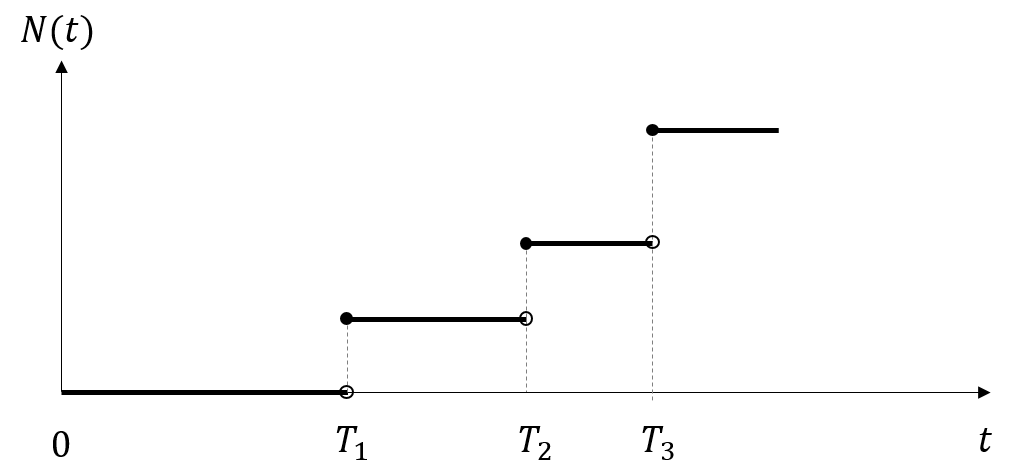
\includegraphics[width=0.7\linewidth]{../figures/stochasticProcess/stochasticProcess/poissonProcessTrajectory}
\caption{A typical realized trajectory from the Poisson process with jumps at $T_1,T_2,$ and $T_3$.}
\label{fig:poissonProcessTrajectory}
\end{figure}


\begin{lemma}[basic properties of Poisson process]\label{ch:theory-of-stochastic-process:th:PoissonProcessbasicproperties}
	Let $N(t)$ be a Poisson process with rate $\lambda$, then:
	\begin{itemize}
		\item $N(t) \sim Poission(\lambda t)$, that is
		$$P(N(t) = k) = \frac{e^{\lambda t}(\lambda t)^k}{k!}$$
		\item $N(t_2)-N(t_1) = N(t_2-t_1) \sim Poisson(\lambda(t_2-t_1))$
		\item $$E[N(t)] = \lambda t, Var[N(t)] = \lambda t, M_{N(t)}(s) = \exp(\lambda t(e^s-1))$$
		\item Jump probability within $[t,t+\Delta t]$: let $\Delta N = N(t+\Delta t) - N(t)$, we have
		$$Pr(\Delta N = n) = \frac{(\lambda\Delta t)^n}{n!} \exp(-\lambda \Delta t) = \frac{(\lambda\Delta t)^n}{n!}(1 - \lambda\Delta t + \frac{(\lambda \Delta t)^2}{2} + \cdots),$$
		or explicitly
		$$Pr(\Delta N = n) = \begin{cases*}
		1 - \lambda\Delta t + O((\Delta t)^2, n = 0\\
		\lambda\Delta t + O((\Delta t)^2, n = 1\\
		O((\Delta t)^2, n\geq 2
		\end{cases*}.$$
	\end{itemize}
\end{lemma}
\begin{proof}
	Directly from definition and the sum property of independent Poisson distribution(\autoref{ch:theory-of-statistics:th:sumofPoisson})and basic property of Poisson distribution(\autoref{ch:theory-of-statistics:th:PoissonBasicproperty}).
\end{proof}

\begin{lemma}[additivity of Poisson process]
	Let $N_1(t)$ and $N_2(t)$ be independent Poisson processes with rate $\lambda_1$ and $\lambda_2$, then
	$N(t) = N_1(t) + N_2(t)$ is a Poisson process with rate $\lambda_1 + \lambda_2$.
\end{lemma}
\begin{proof}
	Use the moment generating function for $N_1(t)$ and $N_2(t)$.(\autoref{ch:theory-of-statistics:th:sumofPoisson}).
\end{proof}

\subsection{Arrival and Inter-arrival Times}
\begin{lemma}[waiting time distribution]
	Let $N(t)$ be a Poisson process with rate $\lambda$. Let $X_1$ be the time of the first arrival. Then 
	$$P(X_1 > t) = \exp(-\lambda t), f_{X_1}(t) = \lambda \exp(-\lambda t)$$
	Similarly, let $X_n$ be the waiting time between the arrival of $n$ after the $n-1$ arrival, then
	$$P(X_n > t) = \exp(-\lambda t)$$
\end{lemma}
\begin{proof}
	(1)From the definition of Poisson process, the $N(t)-N(0) \sim Poisson(\lambda t)$. Then
	$$P(X_1 > t) = P(N(t)-N(0) = 0 ) = (\lambda t)^0 e^{-\lambda t}/0! = e^{-\lambda t}$$
	(2) Using the independent increment property of Poisson process.
\end{proof}

\begin{remark}
	Note that the waiting time distribution is an exponential distribution with parameter $\lambda$, whose mean is $1/\lambda$.
\end{remark}


\begin{lemma}[Arrival times for Poisson processes]\label{ch:theory-of-stochastic-process:th:arrivaltimepoissonprocess}
	If $N(t)$ is a Poisson process with rate $\lambda$, then the arrival time $T_1,T_2,...$ have $T_n\sim Gamma(n,\lambda)$ distribution:
	$$f_{T_n}(t) = \frac{\lambda^nt^{n-1}e^{-\lambda t}}{(n-1)!}$$
	Moreover, we have $E[T_n] = n/\lambda, Var[T_n] = n/\lambda^2$.
\end{lemma}
\begin{proof}
	Let random variables $X_1,X_2,...$ be the interarrival time, then
	\begin{align*}
	T_1 &= X_1 \\
	T_2 & = X_1 +X_2\\
	T_2 & = X_1 +X_2 + X_3\\
	\dots & \dots
	\end{align*}
	Since $X_i$ has exponential distribution(which is $Gamma(1,\lambda)$), the $T_n$ will be $Gamma(n,\lambda)$ distribution(which can be showed that the $n$th power of mgf of exponential function equal to the mgf of Gamma distribution.) Also see property of Gamma distribution(\autoref{ch:theory-of-statistics:th:sumofGamma}.) 
\end{proof}




\begin{mdframed}
	\begin{remark}[Simulating a Poisson process]
		We first generate iid random variables $X_1,X_2,X_3,...$, where $X_i\sim Exp(\lambda)$. Then the arrival times are given as
		\begin{align*}
		T_1 &= X_1 \\
		T_2 & = X_1 +X_2\\
		T_2 & = X_1 +X_2 + X_3\\
		\dots & \dots
		\end{align*}	
	\end{remark}
\end{mdframed}

\begin{lemma}\cite[468]{shreve2004stochastic2}
	Let $N(t)$ be a Poisson process with intensity $\lambda$. We define the \textbf{compensated Poisson process} as $$M(t) = N(t) - \lambda t.$$
	Then $M(t)$ is a martingale.
\end{lemma}
\begin{proof}
	\begin{align*}
	E[M(t)|\cF_s] &= E[M(t)-M(s)|\cF_s] + E[M(s)|\cF_s]\\
	&= E[N(t) - N(s) -\lambda(t-s)|\cF_s] + M(s)\\
	&= E[N(t) - N(s)] -\lambda(t-s) + M(s) \\
	&= M(s).
	\end{align*}
\end{proof}


\subsection{Compound Poisson process}
\begin{definition}[compound Poisson process]\index{compound Poisson process}
	A compound Poisson process, parameterized by a rate $\lambda > 0$ and jump size distribution $G$, is a \textbf{continuous-time} process $\{Y(t),t\geq 0\}$ given by
	$$Y(t) = \sum_{i=1}^{N(t)} D_i,$$
	where $\{N(t),t\geq 0\}$ is a Poisson process with rate $\lambda$, and $\{D_i:i\geq 1\}$ are iid random variables, with distribution $G$, which are also independent of $\{N(t)\}$.
\end{definition}


\begin{figure}[H]
\centering
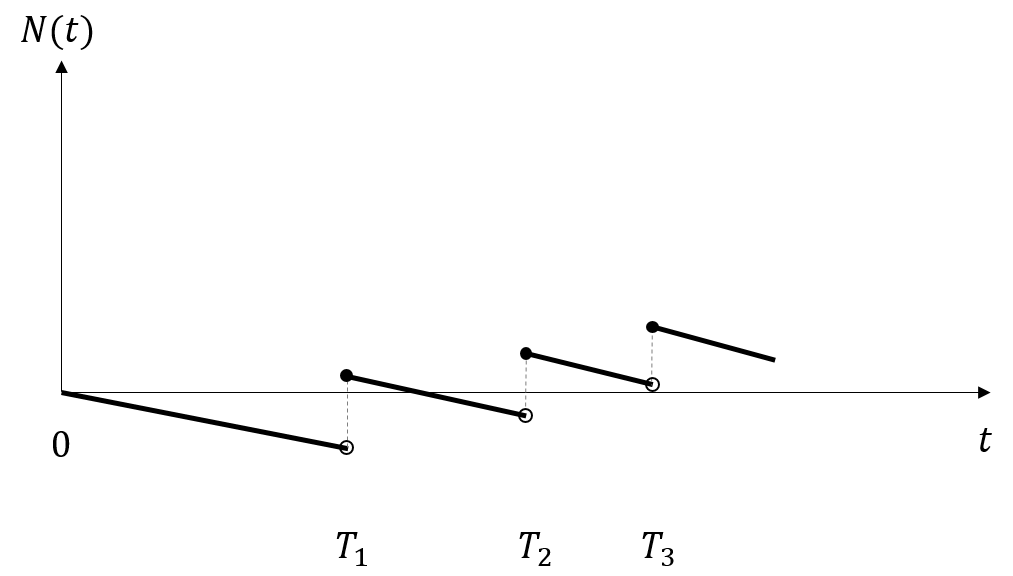
\includegraphics[width=0.7\linewidth]{../figures/stochasticProcess/stochasticProcess/compensatedPoissonProcessTrajectory}
\caption{A typical realized trajectory from the compensated Poisson process with jumps at $T_1,T_2,$ and $T_3$.}
\label{fig:compensatedPoissonProcessTrajectory}
\end{figure}


\begin{remark}[interpretation]
	The jump arrival time distribution and waiting time distribution between two jump events is the same of simple Poisson process; compound Poisson distribution only differs from simple Poisson process in the jump size. 	
\end{remark}




\begin{remark}[reduction to simple Poisson process]
	If we take $D_i$ to be constant 1, then
	$$Y(t)-Y(s) = N(t) - N(s),$$
	that is, $Y(t)$ is the Poisson process.
\end{remark}

\begin{definition}[simple-scaling compound Poisson process]
	Let $N(t)$ be a simple Poisson process, then $Y(t) = \alpha N(t), \alpha \in \R$ is called a simple-scaling compound Poisson process with parameter $\alpha$. 	
	Or equivalently, 
	$$Y(t) = \sum_{i=1}^{N(t)} \alpha.$$	
\end{definition}
\begin{example}
	
\end{example}

\begin{example}[real-world compound Poission process]
	Assume in the stock exchange, the coming of orders follows a compound Poission distribution with strength $\lambda$. For every order, the amount of buying $Z_i$ is iid random sample from random variable $Z$ such that $E[Z] = \mu, Var[Z] = \sigma^2$. Then, the total amount of buying as a function of time is the compound Poission process. 
\end{example}

\begin{lemma}[jump probability within an interval]
	
\end{lemma}



\begin{definition}[compound Poisson distribution]
	Suppose that 
	$N\sim Poisson(\lambda)$ and $X_1,X_2,...$ are iid random variables independent of $N$. Let $Y|N = \sum_{n=1}^N X_n$, then the compound Poisson distribution is distribution of $Y$, which can be obtained by marginalizing the joint distribution $(Y,N)$ over $N$. 
\end{definition}

\begin{lemma}
	$E_Y[Y] = E_N[E_{Y|N}[Y|N]] = E_N[\sum_{i=1}^N E_X[X_i]] = E_N[NE_X[X]] = E_N[N]E_X[X]$.
	
	$$Var[Y] = E_N[Var[Y|N]] + Var_N[E[Y|N]]$$
\end{lemma}

\begin{lemma}[basic properties of compound Poisson process]\label{ch:theory-of-stochastic-process:th:BasicPropertiesOfCompoundPoissonProcess}
	For a compound Poisson process given as
	$$Y(t) = \sum_{i=1}^{N(t)}D_i.$$
	We have
	\begin{itemize}
		
		\item $$E[Y(t)] = E[E[Y(t)|N(t)]] = E[N(t)E[D]] = E[N(t)]E[D] = \lambda t E[D].$$
		\item $$Var[Y(t)] = \lambda t E[D^2].$$
		In particular, if $E[D] = 0$, $$Var[Y(t)] = \lambda t Var[D].$$	
		\item The moment generating function $$M_Y(s) = \exp(\lambda t(M_D(s)-1)),$$
		where $M_D(s)$ is the moment generating function of random variable $D$.
		\item If $Y$ is a simple-scaling compound Poisson process with parameter $\alpha$, then
		$$M_Y(s) = \exp(\lambda t(e^\alpha s-1)).$$
		\item Jump probability within $[t,t+\Delta t]$: let $\Delta N = N(t+\Delta t) - N(t)$, we have
		$$Pr(\Delta N = n) = \frac{(\lambda\Delta t)^n}{n!} \exp(-\lambda \Delta t) = \frac{(\lambda\Delta t)^n}{n!}(1 - \lambda\Delta t + \frac{(\lambda \Delta t)^2}{2} + \cdots),$$
		or explicitly
		$$Pr(\Delta N = n) = \begin{cases*}
		1 - \lambda\Delta t + O((\Delta t)^2, n = 0\\
		\lambda\Delta t + O((\Delta t)^2, n = 1\\
		O((\Delta t)^2, n\geq 2
		\end{cases*}.$$
	\end{itemize}
\end{lemma}
\begin{proof}
	(1)
	$$E[Y(t)] = E[E[Y(t)|N(t)]] = E[N(t)E[D]] = E[N(t)]E[D] = \lambda t E[D].$$
	(2)
	\begin{align*}
	Var[Y(t)] &= E[Var[Y(t)|N(t)]] + Var[E[Y(t)|N(t)]]\\
	&=E[N(t)Var[D]] + Var[N(t)E[D]]\\
	&=Var[D]E[N(t)] + E[D]^2Var[N(t)]\\
	&=Var[D]\lambda t + E[D]^2\lambda t\\
	&=\lambda t(Var[D] + E[D]^2)\\
	&=\lambda t E[D^2]
	\end{align*}	
	(3)
	\begin{align*}
	E[e^{sY}] &= \sum_{i} e^{si}Pr(Y(t) = i) \\
	&=\sum_{i} e^{si}\sum_{n}Pr(Y(t) = i|N(t) = n)Pr(N(t) = n)\\
	&=\sum_n Pr(N(t) = n)\sum_{i} e^{si}\sum_{n}Pr(Y(t) = i|N(t) = n)\\
	&=\sum_n Pr(N(t) = n)\sum_{i} e^{si}Pr(D_1+D_2+...+D_n = i)\\
	&=\sum_n Pr(N(t) = n)(M_D(s))^n\\
	&=\sum_n Pr(N(t) = n)e^{n\ln(M_D(s))}\\
	&=M_{N(t)}(\ln(M_D(s))) \\
	&=\exp(\lambda t(M_D(s)-1))
	\end{align*}
	where we use the fact (\autoref{ch:theory-of-probability:th:additionandscalingtheoremformgf})that the moment generating of $D_1+D_2+...+D_n$ is $(M_D(s))^n$.
	Further, we can use the fact that the Poisson process has moment generating function(\autoref{ch:theory-of-stochastic-process:th:PoissonProcessbasicproperties}) given as
	$$M_{N(t)}(s) = \exp(\lambda t(e^s-1)).$$
	(4)
	For a simple-scaling Poisson compound process, we know that $$M_D(u) = E[\exp(u\alpha)] = \exp(u\alpha). $$
\end{proof}


\begin{lemma}\cite[470]{shreve2004stochastic2}\label{ch:theory-of-stochastic-process:compensatedPoissonProcessIsAMartingale}
	Let $Q(t)$ be a compound Poisson process and let $0 \leq t_0 < t_1 < \dots < t_n$ be given. The increments
	$$Q(t_1)-Q(t_2),Q(t_2)-Q(t_1),\dots,Q(t_n)-Q(t_{n-1}),$$
	are independent and stationary. In particular, the distribution of $Q(t_j) - Q(t_{j-1})$ is the same as the distribution of $Q(t_j - t_{j-1})$.
\end{lemma}
\begin{proof}
	
\end{proof}







\begin{lemma}[decomposition of compound Poisson process when jump size is discrete random variable]\cite[473]{shreve2004stochastic2}
	Assume the jump size $Y$ is a discrete random variable can take finite set of nonzero numbers given by $y_1,\dots,y_M$, and let $p(y_1),...,p(y_M)$ be the associated probability mass. Let $Y_1,\dots$ be a iid random sample of $Y$. Let $N(t)$ be a Poisson process and define the compound Poisson process
	$$Q(t) = \sum_{i=1}^{N(t)} Y_i.$$
	For $m = 1,\dots,M$ let $N_m$ denote the number of jumps in $Q$ of size $y_m$ up to and including $t$. Then,
	$$N(t) = \sum_{m=1}^M N_m(t), Q(t) = \sum_{m=1}^M y_m N_m(t).$$
	The processes $N_m(t), m=1,\dots,M$ defined this way are independent simple Poisson processes with intensity $\lambda p(y_m)$, and $y_1N_1(t),\dots,y_mN_m(t)$ are independent simple-scaling compound Poisson processes. 
\end{lemma}
\begin{proof}
	Note that the moment generating function for $Y$ is given by
	$$M_Y(u) = \sum_{i=1}^m p(y_i)\exp(uy_i).$$
	And the moment generating function for $Q(t)$ is given by
	$$M_{Q(t)}(u) = \exp(\lambda t (\sum_{i=1}^m p(y_i)\exp(uy_i) -1)).$$
	
	On the other hand, the moment generating function for $y_m N_m(t)$ is
	$$M_m(u) = \exp(\lambda p(y_m) t (\exp(u y_m) - 1)).$$
	
	It is easy to see
	$$M_{Q(t)}(u) = \prod_{i=1}^M M_m(u).$$
\end{proof}


\begin{remark}[interpretation]
	For a compound Poisson process with finite jump size space, we can decompose it into the summation of 'simple' compound Poisson processes, each with constant jump size. 
\end{remark}

\subsection{Compensated Poisson process}

\begin{definition}[compensated Poisson process]\index{compensated Poisson process}\hfill
	\begin{itemize}
		\item Let $N(t)$ be a Poisson process with intensity $\lambda$. The compensated Poisson process is defined by
		$$M(t) = N(t) - \lambda t.$$
		\item 	Let $Q(t)$ be the compound Poisson process. Then the \textbf{compensated compound Poisson process} is defined as $$M_Q = Q(t) - \beta \lambda t,$$
		where $\beta = E[D]$, is a martingale. 
	\end{itemize}	
	
\end{definition}

\begin{lemma}[compensated Poisson process is a martingale]\cite[467]{shreve2004stochastic2}
	Let $N(t)$ be a Poisson process with intensity $\lambda$. The compensated Poisson process $M(t) = N(t) - \lambda t$ is a martingale.
\end{lemma}
\begin{proof}
	Let $0\leq s < t$ be given. 
	\begin{align*}
	E[M(t)|\cF(s)] &= E[M(t)- M(s) + M(s)|\cF(s)] \\
	&= E[M(t)- M(s)|\cF(s)] + M(s)\\
	&= E[N(t)- N(s) + \lambda(t-s)|\cF(s)] + M(s)\\
	& = 0 + M(s) \\
	&=M(s)
	\end{align*}
\end{proof}

\begin{lemma}[compensated compound Poisson process is a martingale]\cite[470]{shreve2004stochastic2}
	Let $Q(t)$ be the compound Poisson process. Then the \textbf{compensated compound Poisson process} $$Q(t) - \beta \lambda t$$
	where $\beta = E[D]$, is a martingale. 
\end{lemma}
\begin{proof}
	
\end{proof}

\section{Jump process}

\begin{definition}[right-continuous pure jump process]\index{pure jump process}\cite[475]{shreve2004stochastic2}
	We assume $J$ does not jump at $t=0$ and has only finitely many jumps on each finite interval, and is constant between jumps.
\end{definition}




\begin{remark}[right-continuous vs. left continuous]\hfill \label{ch:theory-of-stochastic-process:remark:purejumpprocess}
	\begin{itemize}
		\item 	By right-continuous, we mean $J(t) = \lim_{s\to t^+}(s)$(but not $J(t) = \lim_{s\to t^-}(s)$) for all $t\geq 0$. The left-continuous counterpart of $J(t)$, denoted as $J(t-)$ can be constructed/modified from $J(t)$ such that at all jumps $J(t) = \lim_{s\to t^-}(s)$ but not $J(t) = \lim_{s\to t^+}(s)$. 
		\item 	If $J$ has a jump at time $t$, then $J(t)$ is the value of $J$ immediately after the jump, and $J(t-)$ is the value immediately before the jump. 
	\end{itemize}
\end{remark}

\begin{example}\hfill
	\begin{itemize}
		\item A Poisson process and a compound Poisson process are pure jump processes because of the Constancy between jumps.
		\item A compensated Poisson process is not a pure jump process because it is decreasing between jumps.
	\end{itemize}	
\end{example}


\begin{definition}[jump difference operator]
	Given a stochastic process $X(t)$, we define the jump difference operator $\Delta$ as
	$$\Delta X(t)  = X(t) - X(t-).$$
	
	If $X(t)$ is a right-continuous process containing jumps at $t_1,t_2,...,t_N$ with jump size $D_1,D_2,...,D_N$, then
	$$\Delta X(t) = \begin{cases*}
	D_i, t=t_i,i=1,2,...,N\\
	0, otherwise
	\end{cases*}$$	
	
	Note that for a continuous process $R(t)$, $\Delta R(t) = 0.$
\end{definition}



\begin{lemma}
	Let $J(t)$ be a right-continuous pure jump process, let $X$ be a left-continuous process(possibly contains jumps), then
	$$\int_0^t X(s-)dJ(s) = \int_0^t X(s)dJ(s) + \int_0^t \Delta X(s) dJ(s),$$
	where $\Delta X(s) = X(s) - X(s-)$.
	In particular, 
	$$\int_0^t J(s-)dJ(s) = \int_0^t J(s)dJ(s) + \int_0^t \Delta J(s) dJ(s).$$
	
	$$\int_0^t X(s)dJ(s-) = 0.$$
	$$\int_0^t X(s-)dJ(s-) = 0.$$
	
	$$\int_0^t J(s)dX^c = 0, \int_0^t J(s-)dX^c = 0 $$
\end{lemma}
\begin{proof}
	(1)Based on definition, we have
	$$X(s) = \Delta X(s) + X(s-).$$
	$$\int_0^t X(s-)dJ(s) = \sum_{0<s\leq t} (X^c(s-) + J(s-))\Delta J(s) = \sum_{0<s\leq t} X^c(s-)\Delta J(s),$$
	where we use the fact that at any jump time $\tau$, $J(\tau-) = 0$, $\Delta J(\tau) \neq 0$.
	(2)From the definition, 
	$$\int_0^t X(s)dJ(s-) = \sum_{0<s\leq t} X(s)\Delta J(s-) = \sum_{0<s\leq t} X(s)(J(s-) - J(s-)) = 0.$$
	(3) From Riemann integral, to integrate a function with finitely many jumps is equivalent to integrate the continuous portion of the integral. Since the continuous portion of $J$ is zero, therefore $\int_0^t J(s)dX^c = 0$. The same arguments apply to $\int_0^t J(s-)dX^c = 0$.
\end{proof}



\begin{definition}[jump process]\index{jump process}\cite[475]{shreve2004stochastic2}
	A stochastic process $X(t)$ defined as
	$$X(t) = X(0) + I(t) + R(t) + J(t),$$
	is called a \textbf{jump process},
	where $X(0)$ is a nonrandom initial condition, $I(t) = \int_0^t \Gamma(s)dW(s)$ is the Ito integral of an adapted process $\Gamma(s)$ with respect to a Brownian motion $W(t)$. $R(t)$ is a Riemann integral given as
	$R(t) = \int_0^t \theta(s)ds$ for some adapted process $\theta(t)$ with respect to the Brownian motion.
	And $J(t)$  is an adapted, \textbf{right-continuous} pure jump process with $J(0) = 0$.
	The continuous part of $X(t)$ is denoted by $X^c(t)$, given by
	$$X^c(t) = X(0) + I(t) + R(t).$$
\end{definition}


\begin{remark}[understand continuity]
	A jump process $X(t)$ is a right-continuous and adapted. The left-continuous counterpart is defined as
	$$X(t-) = X(0) + I(t)  + R(t) + J(t-).$$
	The jump size of $X$ at time $t$ is denoted as
	$$\Delta X(t) = X(t) - X(t-) = J(t) - J(t-) = \Delta J.$$
	If $X(t)$ is continuous, then $\Delta X(t) = 0$. If $X(t)$ has a jump at $t$, then $\Delta X(t)$ is the size of the jump, which equals $\Delta X(t)= J(t) - J(t-)$. 
	We always assume there is no jump at $t = 0$; therefore $\Delta X(0) = 0.$
\end{remark}

\begin{definition}[stochastic integral respect to jump process]\cite[475]{shreve2004stochastic2}
	Let $X(t)$ be a jump process given by
	$$X(t) = X(0) + I(t) + R(t) + J(t).$$
	Let $\Phi(s)$ be an adapted process. The stochastic integral of $\Phi$ respect to $X$ is defined as
	$$\int_0^t \Phi(s)dX(s) = \int_0^t \Phi(s)\Gamma(s)dW(s) + \int_0^t \Phi(s)\theta(s)ds + \sum_{0< s\leq t} \Phi(s)\Delta J(s).$$
	In differential form, we have
	$$\Phi(t)dX(t) = \Phi(t)dI(t) + \Phi(t)dR(t) + \Phi(t) dJ(t)$$
	where
	$$\Phi(t)dI(t) = \Phi(t)\Gamma(t)dW(t), \Phi(t)dR(t) = \Phi(t)\Theta(t)dt.$$
\end{definition}


\begin{remark}[interpretation]\hfill
	\begin{itemize}
		\item $dJ(t)$ should be interpreted as $dJ(t) = J(t+\Delta t) - J(t)$, which is a random variable. If there is a jump at $\tau\in [t,t+\Delta t]$, then $dJ(t) = J(\tau) - J(\tau-)$; If there is no jumps, then $dJ(t) = 0$; moreover, the probability of one jump increment is given by $\lambda d t$, the probability of no jump is $1- \lambda d t$; more than one jump is zero as $\Delta t\to 0$(See the definition of Poisson process in terms of rate functions \autoref{ch:theory-of-stochastic-process:th:BasicPropertiesOfCompoundPoissonProcess}).
		\item The summation $\sum_{0< s\leq t} \Phi(s)\Delta J(s)$ is equivalent to summation of finite terms since there are only finitely many jumps in the interval $[0,t]$. 
	\end{itemize}
\end{remark}




\begin{lemma}[basic properties stochastic integral with jump process]\hfill
	
	\begin{itemize}
		\item Let $N(t)$ be a simple Poisson process. let $\theta(t)$ be a continuous function. Then
		$$\int_0^t \theta(s) dN(t) = \sum_{0<s\leq t} \theta(s)\Delta N(s),$$
		where $\Delta N(s) = 1$ if there is a jump at time $s$.
		
		
		\item Let $N(t)$ be a simple Poisson process, then we have
		$$\int_0^t \Delta N(s)dN(s) = N(t)$$
		$$\int_0^t \Delta(N(s) + \theta(s))dN(s) = N(t)$$
		where $\theta(t)$ is a continuous nonrandom function.
		\item Let $J(t)$  be a compound Poisson process $J(t) = \sum_{i=1}^{N(t)} D_i$, then
		$$\int_0^t \Delta(J(s) + \theta(s))dJ(s) = G(t),$$
		where $G(t)$ is the new compound Poisson process $G(t) = \sum_{i=1}^{N(t)} D_i^2$.	 
	\end{itemize}
\end{lemma}
\begin{proof}
	(1)Note that $\Delta N(t)$ is a jump  indicator process: it takes value 1 when there is a jump; otherwise 0. Therefore, $\int_0^t \Delta N dN = \sum_{0<s\leq t} \Delta N(s)\Delta N(s) = N(t)$ is counting the total jump up to $t$. In addition, use $\Delta \theta = 0$.
	(2) $$\int_0^t \Delta(J(s) + \theta(s))dJ(s) = \sum_{0<s\leq t} \Delta J(s) \Delta J(s)  = \sum_{i=1}^{N(t)} D_i^2.$$
	
\end{proof}

\begin{example}
	Let $X(t) = N(t) - \lambda t$, where $N(t)$ is a Poisson process with intensity $\lambda$. In this case, we have $I(t) = 0, R(t) = -\lambda t$ and $J(t) = N(t)$. Let $\Phi(s) = N(s)$(i.e., $\Phi(s)$ is 1 if $N$ has a jump at time $s$ and $\Phi(s) = 0$ otherwise). Then
	$$\int_0^t \Phi(s)dN(s) = \sum_{0<s\leq t} \Phi(s)\Delta J = \sum_{0<s\leq t} \Delta N\Delta N = N(t),$$
	where use the fact that $\Delta R = 0.$
	Note that $\Delta N(t)$ is a jump  indicator process: it takes value 1 when there is a jump; otherwise 0. Therefore, $\int_0^t \Delta N dN = \sum_{0<s\leq t} \Delta N(s)\Delta N(s) = N(t)$ is counting the total jump up to $t$.
\end{example}



\begin{theorem}[Martingale property for left-continuous integrand]\cite[477]{shreve2004stochastic2}\label{ch:theory-of-stochastic-process:th:leftcontinuousintegrandMartingale}
	Assume that the jump process $X(t) = X(0) + I(t) + R(t) + J(t)$ is a martingale, the integral $\Phi(s)$ is \textbf{left-continuous} and adapted, and 
	$$E[\int_0^t\Gamma^2(s)\Phi(s)^2 ds < \infty, \forall t \geq 0],$$
	then the stochastic integral $\int_0^t \Phi(s)dX(s)$ is also a martingale. That is
	$$E[\int_0^t \Phi(s)dX(s)|\cF_h] = \int_0^h \Phi(s)dX(s)$$
	$$E[\int_0^t \Phi(s)dX(s)] = \Phi(0)X(0).$$
\end{theorem}



\begin{remark}[generalization of Ito integral property]
	We know that the Ito integral 
	$$I(t) = E[\int_0^t\Phi(s)dW(s)]$$
	is a martingale(\autoref{ch:theory-of-stochastic-process:th:ItointegralasMartingale}). 
\end{remark}



\subsection{Quadratic variations}
\begin{lemma}\cite[481]{shreve2004stochastic2}
	Let  $X(t) = X(0) + I(t) + R(t) + J(t)$ be the jump process, then
	$$dXdX = dIdI + dJdJ = \Gamma^2dt + dJdJ, dJdI = 0$$
	The quadratic variation is given as
	$$\int_0^t dX(s)dX(s) = \int_0^t\Gamma^2ds + \sum_{0<s\leq t} (\Delta J_1(s))^2$$
\end{lemma}
\begin{proof}
	To show $dJdI = 0$, we can partition the interval $[0,t]$ into $n$ intervals, then 
	\begin{align*}
	&\abs{\sum_{j=0}^{n-1} (I(t_{j+1}) - I(t_j))(J(t_{j+1})-J(t_j)} \\
	&\leq \max_{0\leq j\leq n-1} \abs{I(t_{j+1}) - I(t_j)} \cdot \sum_{j=0}^{n-1} \abs{J(t_{j+1}) - J(t_j)}\\
	&\leq \max_{0\leq j\leq n-1} \abs{I(t_{j+1}) - I(t_j)} \cdot \sum_{0<s\leq T}\abs{\Delta J(s)}
	\end{align*}
	Note that as $n \to \infty$, $\max_{0\leq j\leq n-1} \abs{I(t_{j+1}) \to 0}$ due to continuity, but $\sum_{0<s\leq T}\abs{\Delta J(s)}$ remains finite.
\end{proof}


\begin{lemma}\cite[481]{shreve2004stochastic2}
	Let  $X_1(t) = X_1(0) + I_1(t) + R_1(t) + J_1(t)$ and $X_2(t) = X_2(0) + I_2(t) + R_2(t) + J_2(t)$  be the jump processes. We further assume $I_1$ and $I_2$ are driven by different Brownian motions with correlation coefficient $\rho_{12}$. Then
	$$dX_1dX_2 = dI_1dI_2 + dJ_1dJ_2 = \Gamma_1\Gamma_2\rho_{12}dt + dJ_1dJ_2.$$
	The quadratic variation is given as
	$$\int_0^t dX(s)dX(s) = \int_0^t\Gamma_1(s)\Gamma_2(s)\rho_{12}ds + \sum_{0<s\leq t} \Delta J_2(s)\Delta J_1(s)$$
\end{lemma}


\begin{remark}[interpretation]
	Note that $\Delta J_1(s) \Delta J_2(s)$ has value only if the two pure jump process has the same jump time.
	
\end{remark}


\subsection{Ito rule}
\begin{lemma}[1D Ito rule]\cite[484]{shreve2004stochastic2}
	Let $X(t)$ be a jump process and $f(x,t)$ a function for which $\frac{\Pa}{\Pa t}f$, $\frac{\Pa}{\Pa x}f$ and $\frac{\Pa^2}{\Pa x^2}f$ are defined and continuous. Then
	$$df = \frac{\Pa}{\Pa t}f dt + \frac{\Pa}{\Pa x}fdX^c + \frac{1}{2}\frac{\Pa^2}{\Pa x^2}f dX^cdX^c + \Delta f(X(t),t)$$
	where $\Delta f(X(t),t) = f(X(t),t) - f(X(t-),t-)$ and $X^c(t) = X^c(0) + I(t) + R(t)$.
	In the integral form, we have
	\begin{align*}
	f(X(t)) &= f(X(0)) + \int_0^t\frac{\Pa}{\Pa s}f ds +\\
	&\int_0^t\frac{\Pa}{\Pa x}dX^c + \frac{1}{2}\int_0^t \frac{\Pa^2}{\Pa x^2}f dX^cdX^c + \sum_{0<s\leq t} f(X(s),s) - f(X(s-),s-).
	\end{align*}
	
\end{lemma}


\begin{remark}[interpretation]
	If the process $X(t)$ does not contain any jumps, or discontinuities, then $$\sum_{0<s\leq t} f(X(s),s) - f(X(s-),s-) = 0.$$
	As a consequence, the Ito rule reduce to the canonical Ito rule for continuous processes.
\end{remark}

\begin{remark}[differentiation]
	$\frac{\Pa}{\Pa x}f(t,x)$ is equivalent to $\frac{\Pa}{\Pa x^c}f(t,x)$;that is, we only take the differential for the continuous process part. This is because for pure jump process will take constant value except at finitely many values, and such effect has been taken care by the final summation.
\end{remark}


\begin{example}[geometric Poisson process]
	Consider the geometric Poisson process 
	$$S(t)  = S(0)\exp(N(t)\log(\sigma+1) - \lambda \sigma t) = S(0)e^{-\lambda\sigma t}(\sigma+1)^{N(t)},$$
	where $\sigma > -1$. We can show the geometric Poisson process is a martingale.
	Then,
	\begin{align*}
	S(t) &= S(0) + \int_0^t S_t ds + \sum_{0<u\leq t}[S(u) - S(u-)]\\ 
	&= S(0) - \lambda\sigma \int_0^t S(u)du + \sum_{0<u\leq t} \sigma S(u-) \\
	&= S(0) - \lambda\sigma \int_0^t S(u-)du + \int_0^t \sigma S(u-) dN(u) \\
	& = S(0) - \int_0^t S(u-)dM(u), M(u) = N(u) - \lambda\sigma t.
	\end{align*}
	
	
	
	Note that we use the fact that $\Pa_{X^c} S = 0$ and $S(u) - S(u-) = S(0)e^{-\lambda \sigma t} = \sigma S(u-)$, where $S(u-) = S(0)e^{-\lambda \sigma t}$ since $N(t-) = 0$(\autoref{ch:theory-of-stochastic-process:remark:purejumpprocess}).
	
	Then, we can show
	$$E[S(t)] = S(0) + E[\int_0^t S(u-)dM(u)] = S(0)$$
	due to \autoref{ch:theory-of-stochastic-process:th:leftcontinuousintegrandMartingale}.
\end{example}

\begin{lemma}[2D Ito rule]\cite[489]{shreve2004stochastic2}
	Let $X(t)$ be a jump process and $f(x,t)$ a function for which $\frac{\Pa}{\Pa t}f$, $\frac{\Pa}{\Pa x}f$ and $\frac{\Pa^2}{\Pa x^2}f$ are defined and continuous. Then
	$$df = \frac{\Pa}{\Pa t}f dt + \frac{\Pa}{\Pa x}dX^c + \frac{1}{2}\frac{\Pa^2}{\Pa x^2}f dX^cdX^c + \Delta f(X(t),t)$$
	where $\Delta f(X(t),t) = f(X(t),t) - f(X(t-),t-)$ and $X^c(t) = X^c(0) + I(t) + R(t)$.
	In the integral form, we have
	\begin{align*}
	f(t,X_1(t),X_2(t))& = f(0,X_1(0),X_2(0)) + \int_0^t f_t ds + \\ &\int_0^tf_{x_1}dX^c_1 +\int_0^tf_{x_2}dX^c_2 + \frac{1}{2}\int_0^t f_{x_1,x_1} dX^c_1dX^c_1 + \frac{1}{2}\int_0^t f_{x_2,x_2}\\ &dX^c_2dX^c_2+\int_0^t f_{x_1,x_2} dX^c_1dX^c_2 + \\
	&\sum_{0<s\leq t} f(s,X_1(s),X_2(s)) - f(s-,X_1(s-),X_2(s-)).
	\end{align*}
\end{lemma}


\begin{lemma}[Ito product rule]
	\begin{align*}
	X_1(t)X_2(t) &= X_1(0)X_2(0) + \int_0^t X_2(s)dX_1^c + \int_0^t X_1(s)dX_2^c(s) + \int_0^t dX_1^c(s)dX_2^c(s) +\\ 
	&\sum_{0<s\leq t}[X_1(s)X_2(s) - X_1(s-)X_2(s-)]\\
	&=X_1(0)X_2(0) + \int_0^t X_2(s-)dX_1 + \int_0^t X_1(s-)dX_2(s) + \int_0^t dX_1(s)dX_2(s)
	\end{align*}
\end{lemma}





\section{Levy processes}
\begin{definition}[infinitely divisible]
	A random variable $X$ is infinitely divisible if its law $p_x$ is infinitely divisible; that is, $X = Y_1^{(n)}+Y_2^{(n)}+\cdots+Y_n^{(n)}$, where $Y_1^{(n)},...,Y_n^{(n)}$ are iid random variables for each $n\in \cN$. In other words, the characteristic function of $X$ can be written as
	$$\Psi_X(u) = (\Phi_{Y_1^{(n)}}(u))^n.$$
\end{definition}

\begin{remark}
	The superscript $(n)$ does not represent any power exponent; it just means when we choose different $n$ to divide the Levy process, we need to have different $Y$ as building blocks.
\end{remark}

\begin{example}[Gaussian random variable]
	Let $X$ have distribution $N(\mu,\sigma^2)$. Then $X$ has characteristic function 
	$$\Phi_X(u) = \exp(i\mu t - \frac{1}{2}\sigma^2u).$$
	$X$ is infinitely divisible with $Y^{(n)}_j\sim N(\mu/n,\sigma^2/n)$, with 
	$$\Phi_Y(u) = \exp(i\mu t/n - \frac{1}{2}\sigma^2u/n) = \Phi_X(u)^{1/n}.$$ 
\end{example}

\begin{example}[Poisson random variable]
	Let $X$ have distribution $Poisson(\lambda)$. Then $X$ has characteristic function 
	$$\Phi_X(u) = \exp(\lambda (e^{iu} - 1)).$$
	$X$ is infinitely divisible with $Y^{(n)}_j\sim Poisson(\lambda/n$, with 
	$$\Phi_Y(u) = \exp(\lambda (e^{iu} - 1)/n) = \Phi_X(u)^{1/n}.$$ 
\end{example}


\begin{definition}[Levy symbol, characteristic exponent]
	Let $X$ be a random variable, let $\Psi_X(u)$ be its characteristic function, then 
	$$\eta = \ln(\Psi_X(u))$$
	is called the Levy symbol or Characteristic exponent. 
\end{definition}


\begin{definition}[cadlag]\index{cadlag}
	Let $(M,d)$ be a metric space, and let $E\subseteq \R$. A function $f: E\to M$ is called a cadlag function if, for every $t\in E$,
	\begin{itemize}
		\item the left limits $f(t^-) = \lim_{s\to t^-}$ exists;
		\item the right limits $f(t^+) = \lim_{s\to t^+}$ exists and equals $f(t)$.
	\end{itemize}
	That is, $f$ is right-continuous with left limits. 
\end{definition}



\begin{definition}[Levy process]\index{Levy process}
	Let $X_t$ be a stochastic process. Then $X_t$ is a Levy process if the following condition are satisfied:
	\begin{enumerate}
		\item $X_0 = 0$.
		\item $X_t$ has independent increments: $L_t - L_s$ is independent of $\cF_s, 0\leq s < t <\infty$.
		\item $L$ has stationary increments: $P(L_t-L_s \leq x) = P(L_{t-s}\leq x), 0 \leq s < t <\infty.$
		\item $L_t$ is continuous in probability: $\lim_{t\to s} L_t = L_s$; that is
		for all $\epsilon > 0$ and for all $s\geq 0$, 
		$$\lim_{t\to s} P(\abs{X(t) - X(s)} > a) = 0.$$ 
	\end{enumerate}
\end{definition}

\begin{remark}[continuity of sample path]\hfill
	\begin{itemize}
		\item Note that in the Levy processes, the sample path is continuous in probability, while in Wiener process, the sample path is almost surely continuous.
		\item If $X_t$ is a Levy process, then one may show that the sample path is almost surely right continuous with left limits(cadlag). 
	\end{itemize}
\end{remark}


\begin{remark}[Levy process is infinitely divisible]
	From property(2)(3) in the definition, we know that a Levy process $X_t$ is infinitely divisible.
\end{remark}

\begin{lemma}
	If $X_t$ is a Levy process, then $X_t$ is infinitely divisible for each $t\geq 0$. Furthermore,
	$$\Psi_{X(t)}(u) = e^{t\eta(u)}$$
	where $\eta$ is the Levy symbol of $X(1)$, i.e., $\eta = \ln(\Psi_{X(1)}(u)$.
\end{lemma}
\begin{proof}
	From property(2)(3) in the definition, we know that a Levy process $X_t$ is infinitely divisible.
\end{proof}


\begin{definition}[compound Poisson process]\index{compound Poisson process}
	A compound Poisson process, parameterized by a rate $\lambda > 0$ and jump size distribution $G$, is a process $\{Y(t),t\geq 0\}$ given by
	$$Y(t) = \sum_{i=1}^{N(t)} D_i,$$
	where $\{N(t),t\geq 0\}$ is a Poisson process with rate $\lambda$, and $\{D_i:i\geq 1\}$ are iid random variables, with distribution $G$, which are also independent of $\{N(t)\}$.
\end{definition}

\begin{definition}[compound Poisson distribution]
	Suppose that 
	$N\sim Poisson(\lambda)$ and $X_1,X_2,...$ are iid random variables independent of $N$. Let $Y|N = \sum_{n=1}^N X_n$, then the compound Poisson distribution is distribution of $Y$, which can be obtained by marginalizing the joint distribution $(Y,N)$ over $N$. 
\end{definition}

\begin{lemma}
	$E_Y[Y] = E_N[E_{Y|N}[Y|N]] = E_N[\sum_{i=1}^N E_X[X_i]] = E_N[NE_X[X]] = E_N[N]E_X[X]$.
	
	$$Var[Y] = E_N[Var[Y|N]] + Var_N[E[Y|N]]$$
\end{lemma}


\begin{lemma}
	Let $\{Z_n,n\in \cN \}$ be a sequence of iid random variables taking values in $\R^d$ with common law $\mu_Z$ and let $N\sim Poisson(\lambda)$. Let 
	$X = \sum_{i=1}^N Z_i.$ 
	Then, for each $u\in \R^d$, 
	$$\Psi_X(u) = E[e^{iuX}] = \exp(\int_{\R^d} (e^{iu^Ty}-1)\lambda \mu_Z(dy)).$$
\end{lemma}
\begin{proof}
	\begin{align*}
	\Psi_X(u) &= \sum_{n=0}^\infty E[e^{iu^TX}|N=n]P(N=n)\\
	&=\sum_{n=0}^\infty E[e^{iu^TX}|N=n]e^{-\lambda} \frac{\lambda^n}{n!}\\
	&=e^{-\lambda}\sum_{n=0}^\infty \frac{(\lambda\Psi_Z(u))^n}{n!}\\
	&=\exp(\lambda(\Psi_Z(u)-1))
	\end{align*}
	where
	$$\Psi_Z(u) = \int_{\R^d} (e^{iu^Ty}-1) \mu_Z(dy).$$
\end{proof}



\begin{theorem}
	Suppose that $\mu\in \R, \sigma \geq 0$, and $\nu$ is a measure concentrated on $\R/\{0\}$ such that $\int_{\R}\min(1,x^2)\nu(dx) < \infty$. A probability law of a real-valued random variable $L$ has characteristic exponent $\Psi(u) = -\frac{1}{t}\log(E[e^{iuL_t}])$ given by
	$$\Psi(u;t) = \int_{\R} e^{iux}\eta(dx) = e^{-t\Psi(u)},\forall u\in \R$$
	if and only if there exists a triple $(\mu,\sigma,\nu)$ such that
	$$\Psi(u) = i\mu u + \frac{1}{2}\sigma^2 u^2 + \int_R (1-e^{iux} + iux \bm{1}_{\abs{x}<1}) \nu(dx)$$
	for every $u\in\R$.
\end{theorem}

\begin{definition}[Levy measure]
	Levy measure is a measure $\nu$ on $\R^d/\{0\}$ such that
	$$\int\min(\abs{y}^2,1)\nu(dy) < \infty$$
\end{definition}


\begin{remark}[interpretation]\cite{Manuge2015levy}
	The theorem says that there exists a probability space where $L = L^{(1)}+L^{(2)}+L^{(3)}$; $L^{(1)}$ is the standard Brownian motion with drift, $L^{(2)}$ is a compound Poisson process, and $L^{(3)}$ is a square integrable martingale with countable number of jumps of magnitude less than 1(almost surely).
\end{remark}


\begin{example}[Brownian motion]
	Let $B(t)$ be a standard Brownian motion in $\R^d$. Then, $C(t) = bt + \sigma B(t), b\in \R^d, \sigma\in \R^{d\times d}$ is a Levy process with its characteristic function given by 
	$$\Psi_{B(t)}(u) = \exp(t\eta_C(u)),$$
	where $\eta_C(u)$ is Levy symbol of $C(1)$ of the form
	$$\eta_C(u) = ib^T - \frac{1}{2} u^T \sigma^T\sigma u.$$
\end{example}



	\section{Notes on bibliography}
	
	
	For Fokker-Planck equation, see \cite{risken2012fokker}\cite{gardiner2009stochastic}.
	
	\printbibliography
\end{refsection}

\begin{refsection}
	\startcontents[chapters]


\chapter{Fokker-Planck Equation}\label{ch:fokker-planck-equation}	
\printcontents[chapters]{}{1}{}
\section{Fokker-Planck equations}

\subsection{Formulations: one dimension}
\begin{lemma}[one dimensional Fokker-Planck equation]\cite[121]{chirikjian2011stochastic1}\cite[79]{clark2011foreign}\label{ch:theory-of-stochastic-process:th:oneDFokkerPlanckEquation}\label{ch:theory-of-stochastic-process:th:1DFokkerPlanckEquationAssociatedWithItoSDE}
	The Fokker-Planck equation is associated with an Ito SDE
	$$dx = \mu(x,t) dt + \sigma(x,t) dW_t,$$
	where $W_t$ is a Wiener process, is given as
	$$\frac{\Pa p}{\Pa t} = -\frac{\Pa}{\Pa x}(\mu(x)p)  + \frac{1}{2}\frac{\Pa^2}{\Pa x^2}(\sigma(x,t)^2p),$$
	note that $\mu,\sigma$ can have dependence on both $x$ and $t$.
\end{lemma}
\begin{proof}
	Let $f(x)$ be an arbitrary smooth function of $x$, then
	$$\int f(x)p(x,t) dx = \ip{f} \implies \int f(x)\frac{\Pa p}{\Pa t} dx = \ip{\frac{d f}{d t}}.$$
	Note that from Ito rule, we have
	\begin{align*}
	df &= \frac{df}{dx} dx + \frac{1}{2}\frac{d^2f}{dx^2} \sigma^2 dt \\
	df &= \frac{df}{dx} (\mu(x,t) dt + \sigma(x,t) dW_t) + \frac{1}{2}\frac{d^2f}{dx^2} \sigma^2 dt \\
	\implies \ip{df} &= (\frac{df}{dx} \mu(x,t)  + \frac{1}{2}\frac{d^2f}{dx^2} \sigma^2 )dt
	\end{align*}
	Then
	\begin{align*}
	\int f(x)\frac{\Pa p}{\Pa t} dx &= \ip{\frac{d f}{d t}} \\&= \ip{\frac{df}{dx} \mu(x,t)  + \frac{1}{2}\frac{d^2f}{dx^2} \sigma^2}\\
	&=\int (\frac{df}{dx} \mu(x,t)  + \frac{1}{2}\frac{d^2f}{dx^2} \sigma^2) p(x,t)dx
	\end{align*}
	Integrating by parts(twice) and drop out the surface terms($p(x\to\infty) = 0$), we have
	$$\int f(x)\frac{\Pa p}{\Pa t} dx = \int f(x)(-\frac{\Pa \mu p}{\Pa x} + \frac{1}{2}\frac{\Pa^2 \sigma^2 p}{\Pa x^2})dx$$
	Because $f(x)$ is an arbitrary function, we have
	$$\frac{\Pa p}{\Pa t} = -\frac{\Pa \mu p}{\Pa x} + \frac{1}{2}\frac{\Pa^2 \sigma^2 p}{\Pa x^2}$$
	using fundamental lemma of calculus of variations(\autoref{ch:calculus-of-variations:th:fundamentallemmaofcalculusofvariations}).
\end{proof}

\begin{remark}
	Fokker-Planck equation is also known as Kolmogorov forward equation. 	
\end{remark}

\begin{remark}[common boundary conditions]\cite[92]{pavliotis2014stochastic}\hfill
\begin{itemize}
	\item Adsorbing boundary condition. For example at interval $[0,1]$, we have $p(x=0,t|x_0,t_0) = p(x=1,t|x_0,t_0) = 0$.
	\item Reflecting boundary condition. For example at interval $[0,1]$, we have $\Pa_x p(x=0,t|x_0,t_0) = \Pa_x p(x=1,t|x_0,t_0) = 0$, which are interpreted as zero flux at the boundary.
	\item Periodic boundary condition. For example at interval $[0,1]$, we have $ p(x=0,t|x_0,t_0) = p(x=1,t|x_0,t_0)$.
\end{itemize}

	
\end{remark}

\subsubsection{Formulations: multiple dimension}

\begin{lemma}[multi-dimensional Fokker-Planck equation]\cite[121]{chirikjian2011stochastic1}\cite[83]{clark2011foreign}\label{ch:theory-of-stochastic-process:th:multiDFokkerPlanckEquation}
	The Fokker-Planck equation is associated with a $d$ dimensional Ito SDE
	$$dx_i = \mu_i(x,t) dt + \sum_{j=1}^{m}\sigma_{ij}^2(x,t) dW_j(t),i=1,2,...,d$$
	where $W_i(t),i=1,...,d$ is are multiple dimensional independent Wiener process, is given as
	$$\frac{\Pa p}{\Pa t} = -\sum_{i=1}^d \frac{\Pa}{\Pa x_i}(\mu_i(x) p)  + \frac{1}{2}\sum_{i=1}^d\sum_{j=1}^d \frac{\Pa^2}{\Pa x_i\Pa x_j}(\sum_{k=1}^m \sigma_{ik}\sigma_{jk}p).$$
\end{lemma}
\begin{proof}
Let $G_t$ be a function of $x=(x_1,x_2,...,x_d)$ given by $G_t = g(x_1,x_2,...,x_d)$. From Ito rule, we have
\begin{align*}
dG_t &= \sum_{i=1}^{d} \frac{\Pa g}{\Pa x_i} dx_i + \frac{1}{2}\sum_{i=1}^{d}\sum_{j=1}^{d}\frac{\Pa^2 g}{\Pa x_i\Pa x_j} dx_idx_j \\
&=\sum_{i=1}^{d} \frac{\Pa g}{\Pa x_i} (\mu_i(x,t) dt + \sum_{j=1}^{m}\sigma_{ij}^2(x,t) dW_j(t)) + \frac{1}{2}\sum_{i=1}^{d}\sum_{j=1}^{d}\frac{\Pa^2 g}{\Pa x_i\Pa x_j} \sum_{k=1}^m \sigma_{ik}\sigma_{jk} dt \\
&=(\sum_{i=1}^{d} \frac{\Pa g}{\Pa x_i} \mu_i(x,t) + \frac{1}{2}\sum_{i=1}^{d}\sum_{j=1}^{d}\frac{\Pa^2 g}{\Pa x_i\Pa x_j} \sum_{k=1}^m \sigma_{ik}\sigma_{jk})dt + \sum_{i=1}^{d}\frac{\Pa g}{\Pa x_i} \sum_{j=1}^{m}\sigma_{ij}^2(x,t) dW_j(t) .
\end{align*}

Note that
$$\frac{d}{dt} E[G_t] = \frac{d}{dt}\int_{\R^d} p(x,t)g(x)dx = \int_{\R^d} \frac{d}{dt}p(x,t) g(x)dx.(*)$$

From another aspect, we have
\begin{align*}
\frac{d}{dt}E[G_t] &= E[\frac{d}{dt}G_t] \\
&=E[(\sum_{i=1}^{d} \frac{\Pa g}{\Pa x_i} \mu_i(x,t) + \frac{1}{2}\sum_{i=1}^{d}\sum_{j=1}^{d}\frac{\Pa^2 g}{\Pa x_i\Pa x_j} \sum_{k=1}^m \sigma_{ik}\sigma_{jk})] \\
&=\int_{\R^d}p(x,t)(\sum_{i=1}^{d} \frac{\Pa g}{\Pa x_i} \mu_i(x,t) + \frac{1}{2}\sum_{i=1}^{d}\sum_{j=1}^{d}\frac{\Pa^2 g}{\Pa x_i\Pa x_j} \sum_{k=1}^m \sigma_{ik}\sigma_{jk})]dx \\
&=\int_{\R^d}p(x,t)(\sum_{i=1}^{d} \frac{\Pa g}{\Pa x_i} \mu_i(x,t) + \frac{1}{2}\sum_{i=1}^{d}\sum_{j=1}^{d}\frac{\Pa^2 g}{\Pa x_i\Pa x_j} \sum_{k=1}^m \sigma_{ik}\sigma_{jk})]dx \\
&=\int_{\R^d} [-\sum_{i=1}^{d}\frac{\mu_i(x,t)p(x,t)}{dx_i} + \frac{1}{2} \sum_{i=1}^{d}\sum_{j=1}^{d} \frac{\Pa^2}{\Pa x_i\Pa x_j} \sum_{k=1}^m \sigma_{ik}\sigma_{jk} \sigma_{ik}\sigma_{jk} p(x,t) ] g(x)dx \\
\end{align*}

Combine with $(*)$, we have
$$\int_{\R^d}[\frac{d}{dt}p(x,t)-\sum_{i=1}^{d}\frac{\mu_i(x,t)p(x,t)}{dx_i} + \frac{1}{2} \sum_{i=1}^{d}\sum_{j=1}^{d} \frac{\Pa^2}{\Pa x_i\Pa x_j} \sum_{k=1}^m \sigma_{ik}\sigma_{jk} \sigma_{ik}\sigma_{jk} p(x,t) ] g(x)dx $$
holds for any function $g(x)$. Therefore
	$$\frac{\Pa p}{\Pa t} = -\sum_{i=1}^d \frac{\Pa}{\Pa x_i}(\mu_i(x) p)  + \frac{1}{2}\sum_{i=1}^d\sum_{j=1}^d \frac{\Pa^2}{\Pa x_i\Pa x_j}(\sum_{k=1}^m \sigma_{ik}\sigma_{jk}p).$$
\end{proof}




\subsection{Steady state \& detailed balance}
\begin{lemma}[1d steady state solution]
Given a 1d Fokker-Planck 	$$\frac{\Pa p}{\Pa t} = -\frac{\Pa}{\Pa x}(\mu(x)p)  + \frac{1}{2}\frac{\Pa^2}{\Pa x^2}(\sigma(x,t)^2p),$$
the steady state distribution $p^{eq}$ will satisfy 
$$-\frac{\Pa}{\Pa x}(\mu(x)p)  + \frac{1}{2}\frac{\Pa^2}{\Pa x^2}(\sigma(x,t)p) =0.$$
Let $J = up - \frac{1}{2}\frac{\Pa}{\Pa x}(\sigma(x,t)^2p), $ then the steady state solution is satisfying 
$$\frac{\Pa}{\Pa x} J = 0.$$
In particular, 
\begin{itemize}
	\item If domain $D = [a,b]$, and the boundary are reflecting, then
	we have stronger result of $J = 0$.
	\item If domain $D = [a,b]$, and the boundary are periodic, then
we have stronger result of $J = const $, $const$ might not be zero.
\end{itemize}
\end{lemma}
\begin{proof}
On 1D, $\Pa_x J = 0 \implies J = const.$
\end{proof}


\begin{lemma}[2d/3d steady state solution]
Given a 2d/3d Fokker-Planck equation
$$\frac{\Pa p}{\Pa t} = -\sum_{i=1}^d \frac{\Pa}{\Pa x_i}(\mu_i(x) p)  + \frac{1}{2}\sum_{i=1}^d\sum_{j=1}^d \frac{\Pa^2}{\Pa x_i\Pa x_j}(\sum_{k=1}^m \sigma_{ik}\sigma_{jk}p),$$
the steady state solution is given as
$$-\sum_{i=1}^d \frac{\Pa}{\Pa x_i}(\mu_i(x) p)  + \frac{1}{2}\sum_{i=1}^d\sum_{j=1}^d \frac{\Pa^2}{\Pa x_i\Pa x_j}(\sum_{k=1}^m \sigma_{ik}\sigma_{jk}p)$$
Let $Q_i = \sum_{k}\sigma^{-1}_{ik}(2\mu_k - 2\sum_j \frac{\Pa}{\Pa x_j} \sigma_{kj})$
\end{lemma}


\subsection{Averages and adjoint operator}
\begin{lemma}
In the function space of square-integrable functions and the scalar product is defined by 
$$\ip{f,g} = \int_a^b f(x)\bar{g(x)}dx.$$
Consider a linear differential operator $T$ given as
$$Tu = \sum_{k=0}^n a_k(x)\frac{d^k}{dx^k} u.$$
If $f$ or $g$ vanishes for $x\to a, b$, then the adjoint of $T$ is
$$T^\dagger u = \sum_{k=0}^n (-1)^k \frac{d^k}{\conj{a_k(x)}dx^k} u$$
\end{lemma}
\begin{proof}
Use integration-by-parts.
\end{proof}



\begin{example}
The Sturm-Liouville operator is defined as
$$Lu = -(pu')' + qu.$$
It can be showed that $Lu = L^\dagger u, L = L^\dagger.$
\end{example}

\begin{corollary}[adjoint operators]\hfill
	\begin{itemize}
		\item $$Af = b(x)\frac{d}{dx}f(x), A^{\dagger}f=-\frac{d}{dx}b(x)f(x)$$
		that is,$$\int_{-\infty}^{\infty} g(x)b(x)\frac{d}{dx}f(x) dx = -\int_{-\infty}^{\infty} f(x)\frac{d}{dx}b(x)f(x) dx$$
		\item $$Af = D(x)\frac{d^2}{dx^2}f(x), A^{\dagger}f=\frac{d^2}{dx^2}D(x)f(x)$$
		\item $$Af = \frac{d}{dx}D(x)\frac{d}{dx}f(x), A^{\dagger}f=\frac{d}{dx}D(x)\frac{d}{dx}f(x)c$$
	\end{itemize}
\end{corollary}
\begin{proof}
	(1) use integration by parts, note that $\lim_{x\to\infty} f(x) = 0$.(2)(3) use integration by parts, note that $\lim_{x\to\infty} f(x) = 0$, $\lim_{x\to\infty} \frac{d}{dx}f(x) = 0$.
\end{proof}

\begin{corollary}[Adjoint of Fokker-Planck operator]
	Define 
	$$Af = \sum_{i} b_i(x) \frac{\Pa }{\Pa x}f(x) + \frac{1}{2}\sum_{i,j}(\sigma(x)\sigma(x)')_{ij}\frac{\Pa^2 }{\Pa x_i\Pa x_j}f(x)$$
	and its adjoint is
	$$A^{\dagger}f = -\sum_{i}  \frac{\Pa }{\Pa x}b_i(x)f(x) + \frac{1}{2}\sum_{i,j}\frac{\Pa^2 }{\Pa x_i\Pa x_j}(\sigma(x)\sigma(x)')_{ij}f(x)$$
\end{corollary}

\iffalse
\begin{lemma} Given a Fokker-Planck equation on the probability density of $x$, 
	$$\frac{\Pa}{\Pa t} P(x,t) = -LP(x,t)$$
	with
	$$L = \frac{\Pa}{\Pa x}v(x) - \frac{\Pa}{\Pa x} D \frac{\Pa}{\Pa x},$$
	the solution is
	$$P(x,t) = e^{Lt}P(x,0).$$
Define the average of any dynamic property $A(x(t))$ as

	$$\ip{A(x(t))} = \int dx A(x(t))P(x,t) = \int dx A(x)e^{-Lt}P(x,0)$$
	The adjoint operator is
	$$L^{\dagger} = -v(a)\frac{\Pa}{\Pa t} - - \frac{\Pa}{\Pa x} D \frac{\Pa}{\Pa x}$$
	then
	$$\frac{\Pa}{\Pa t} A(x,t) = -L^{\dagger}A(x,t)$$
	with solution $A(x(t)) = e^{-L^{\dagger}t}A(x(0))$.
\end{lemma}
\begin{proof}
	\begin{align*}
	\ip{A(x(t))} &= \int dx A(x)e^{-Lt}P(x,0) = \sum_{n=0}^\infty \frac{(-t)^n}{n!}\int dx A(x(t))L^n P(x,0) \\
	&= \sum_{n=0}^{\infty} \frac{(-t)^n}{n!} \int dx ((L^\dagger)^nA(x(t))) P(x,0) = \int dx e^{-L^\dagger t}A(x(0)) P(x,0) 
	\end{align*}
\end{proof}


\begin{corollary}
	Define 
	$$G(t|x_0,t_0) = \int_{\Omega} dx P(x,t|x_0,t_0)$$
	where $\Omega$ is the survival region, then
	$$\frac{\Pa }{\Pa t}G(t|x,0) = -\cL_{FP}^{\dagger}G(t|x,0)$$
\end{corollary}

\fi

\subsection{Backward equation}
\begin{lemma}
The backward Fokker-Planck equation is given as
$$\frac{\Pa}{\Pa t_1}P(t_2,y_2|t_1,y_1) = - A(y_1,t_1)\frac{\Pa}{\Pa y_1}P(t_2,y_2|t_1,y_1) - \frac{1}{2}B(y_1,t_1)\frac{\Pa^2}{\Pa y_1^2} P(t_2,y_2|t_1,y_1),$$
where $$\int (z-y_1)P(t_1,z|t-\Delta t,y_1)dz = \Delta t A(y_1,t_1-\Delta t)$$ and $$\int (z-y_1)^2P(t_1,z|t-\Delta t,y_1)dz = \Delta t B(y_1,t_1-\Delta t)$$.
\end{lemma}
\begin{proof}
From Chapman-Kolmogorov equation, we have
	$$P(t_2,y_2|t-\Delta t,y_1) = \int P(t_2,y_2|t_1,z)P(t_1,z|t_1-\Delta t,y_1)dz.$$
	
	Using Taylor expansion, we have
	
	$$P(t_2,y_2|t_1,z) = P(t_2,y_2|t_1,y_1)+\frac{\Pa}{\Pa y_1}P(t_2,y_2|t_1,y_1) (z-y_1) +\frac{1}{2}\frac{\Pa^2}{\Pa y_1^2} (z-y_1)^2 + O(\int(z-y_1)^3. $$
	
	Plug in, we have
	\begin{align*}
	P(t_2,y_2|t_1-\Delta t,y_1) &= P(t_2,y_2|t_1,y_1) - \Delta t \frac{\Pa}{\Pa t_1}P(t_2,y_2|t_1,y_1)\\
	&+ \frac{\Pa}{\Pa y_1}P(t_2,y_2|t_1,y_1)\int (z-y_1)P(t_1,z|t-\Delta t,y_1)dz\\
	&+\frac{1}{2}\frac{\Pa^2}{\Pa y_1^2}\int(z-y_1)^2P(t_1,z|t_1-\Delta t,y_1)dz + \\
	&+O(\int(z-y_1)^3P(t_1,z|t-\Delta t,y_1)dz)
	\end{align*}
	
	
	Let $\int (z-y_1)P(t_1,z|t-\Delta t,y_1)dz = \Delta t A(y_1,t_1-\Delta t)$ and $\int (z-y_1)^2P(t_1,z|t-\Delta t,y_1)dz = \Delta t B(y_1,t_1-\Delta t)$, we have
	$$\frac{\Pa}{\Pa t_1}P(t_2,y_2|t_1,y_1) = - A(y_1,t_1)\frac{\Pa}{\Pa y_1}P(t_2,y_2|t_1,y_1) - \frac{1}{2}B(y_1,t_1)\frac{\Pa^2}{\Pa y_1^2} P(t_2,y_2|t_1,y_1)$$ 
\end{proof}

\begin{remark}[interpretation]\hfill
\begin{itemize}
	\item The backward Fokker-Planck equation describes the dependence of $P(y_2,t_2|y_1,t_1)$ on the initial condition $(y_1,t_1)$.
	\item To be well-posed, the backward Fokker-Planck equation needs a final condition rather than an initial condition.	
\end{itemize}
\end{remark}


\begin{lemma}[Backward equation using adjoint operator]
If 
$$\frac{\Pa }{\Pa t} P(x,t|x_0,t_0) = \cL_x P,$$
then
$$\frac{\Pa }{\Pa t_0} P(x,t|x_0,t_0) = \cL_{x_0} P,$$
\end{lemma}
\begin{proof}
From Chapman-Kolmogorov equation, we have
$$P(x_1,t_1|x_0,t_0) = \int P(x_1,t_1|x,t)P(x,t|x_0,t_0)dx,$$
where $t_0 < t < t_1$. Take the derivative with respect to $t$, then
\begin{align*}
\int [\frac{\Pa}{\Pa t}P(x_1,t_2|x,t)]P(x,t|x_0,t_0) + \int P(x_1,t_2|x,t)\frac{\Pa}{\Pa t}P(x,t|x_0,t_0) = 0\\
\int [\frac{\Pa}{\Pa t}P(x_1,t_2|x,t)]P(x,t|x_0,t_0) + \int P(x_1,t_2|x,t)\cL_{x}P(x,t|x_0,t_0) = 0\\
\int [\frac{\Pa}{\Pa t}P(x_1,t_2|x,t) - \cL_{x}^\dagger P(x_1,t_2|x,t)]P(x,t|x_0,t_0) = 0
\end{align*}
where $\cL^\dagger_x$ is the adjoint operator satisfying

$$\int P(x_1,t_1|x,t)\cL_{x}P(x,t|x_0,t_0) dx = \int [\cL_x^\dagger P(x_1,t_1|x,t)]P(x,t|x_0,t_0)dx. $$
Then
$$\frac{\Pa}{\Pa t}P(x_1,t_2|x,t) - \cL_{x}^\dagger P(x_1,t_2|x,t) = 0.$$
\end{proof}




\begin{lemma}[Backward equation on expectation quantity]\label{ch:fokker-planck-equation:th:FokkerPlanckBackwardEquationOnExpectationQuantity}
Let $u(t,x) = E[g(X_T)|X(t) = x]$. Assume $$\int P(t,y|t-h,x)(y-x)dy = b(x,t)h + o(h)$$ and
$$\int P(t,y|t-h,x)(y-x)^2dy = \sigma(x,t)h + o(h),$$
and higher moment vanish as $h\to 0.$ 
 Then $u$ satisfy 
$$\frac{\Pa u}{\Pa t} + b(x)\frac{\Pa u}{\Pa x} + \frac{1}{2}\sigma^2(x)\frac{\Pa^2 f}{\Pa x^2},$$
with final condition $u(T,x) = g(x)$.
\end{lemma}
\begin{proof}
Note that 
$$u(t,x) = E[g(X_T)|X(t) = x] = \int g(X_T)P(T,X_T|t,x) dX_T$$ and
$$u(t-h,x) = \int E[g(X_T)|X(t) = y]P(t,y|t-h,x) dy$$
$$u(t,x) = \int E[g(X_T)|X(t) = x]P(t,y|t-h,x) dy$$

Therefore,
\begin{align*}
\frac{u(t) - u(t-h)}{h} & = \frac{\int P(t,y|t-h,x)(u(t,y) - u(t,x)}{h}\\
&= \frac{1}{h}\int P(t,y|t-h,x)[(y-x)\frac{\Pa u}{\Pa x} +\frac{1}{2} (y-x)^2\frac{\Pa^2 u}{\Pa x^2}]
\end{align*}
\end{proof}

\begin{remark}
Backward equation can also be derived using Feyman Kac theorem by assuming the stochastic process of $X(t)$(see \autoref{ch:fokker-planck-equation:th:FeymanKacBackwardEquation}).
\end{remark}

\begin{lemma}[Backward equation on expectation quantity using adjoint operator]\label{ch:fokker-planck-equation:th:FokkerPlanckBackwardEquationOnExpectationQuantityUsingAdjointOperator}
	Let $u(t,x) = E[g(X_T)|X(t) = x]$. Assume
	$$\frac{\Pa }{\Pa t} P(x,t|x_0,t_0) = \cL_x P(x,t|x_0,t_0).$$
	Then
	$$\frac{\Pa u}{\Pa t} = \cL_x^\dagger u$$
	with final condition $u(T,x) = g(x)$.
\end{lemma}
\begin{proof}
	Note that 
	$$u(t,x) = E[g(X_T)|X(t) = x] = \int g(X_T)P(T,X_T|t,x) dX_T$$ and
	Therefore,
	\begin{align*}
	\frac{\Pa u(t,x)}{\Pa t} & = \int g(X_T) \frac{\Pa}{\Pa t} P(T,X_T|t,x) dX_T \\
	&= \int g(X_T) \cL_x^\dagger P dX_T = \cL_x^\dagger \int g(X_T)  P dX_T = \cL_x^\dagger u(x,t).
	\end{align*}
\end{proof}

\begin{remark}[analog in Markov chain]
For analog in discrete-time Markov chain, see \autoref{ch:markov-chains:th:KolmogorovbackwardequationDiscreteTimeMarkovChain}.
\end{remark}


\subsection{Mean first passage time problem}



\iffalse
\begin{lemma}
	Given a Stratonovich stochastic differential equation 
	$$dx(t) = v(x) dt + \sqrt{2D}dw(t),$$
	its Fokker-Planck equation is given as
	$$\frac{\Pa}{\Pa t}P(x,t|x_0,t_0) = -\frac{\Pa}{\Pa x}(v(x)P(x,t|x_0,t_0) + \frac{\Pa}{\Pa x}D\frac{\Pa}{\Pa x}P(x,t|x_0,t_0) $$
	
	Note that for \textbf{Markovian system}, we also have
	$$\frac{\Pa}{\Pa t} P(x,t|x_0,t_0) = \frac{\Pa}{\Pa t_0} P(x,t|x_0,t_0).$$
\end{lemma}
\begin{proof}
	(2)
	$$\frac{\Pa}{\Pa t} P(x,t|x_0,t_0) = \frac{\Pa}{\Pa t} P(x,t-t_0|x_0,0) = -\frac{\Pa}{\Pa t_0} P(x,t-t_0|x_0,0) = -\frac{\Pa}{\Pa t_0}P(x,t|x_0,t_0).$$	
\end{proof}
\fi



\begin{definition}[survival probability]
	The survival probability up to $t$ in domain $\Omega$ is given as
	$$G(t|x_0,t_0) = \int_{\Omega} dx P(x,t|x_0,t_0).$$
	Or equivalently, 
	$$G(t|x_0,0) = Pr(\tau > t) = \int_t^{\infty} \rho(\tau|x_0,0)$$
	where $\rho(\tau|x_0,0)$ is the probability density for the first passage time $\tau$ starting from $x_0$ at $t = 0$.
\end{definition}

\begin{lemma}[survival probability governing equation]
Assume
$$\frac{\Pa }{\Pa t} P(x,t|x_0,t_0) = -\cL_x P(x,t|x_0,t_0).$$
Then
	$$\frac{\Pa }{\Pa t}G(t|x,0) = -\cL_{x}^{\dagger}G(t|x,0),$$
where $\cL_x^\dagger$ is the adjoint operator of $\cL_x$.
\end{lemma}
\begin{proof}
Use the theorem(\autoref{ch:fokker-planck-equation:th:FokkerPlanckBackwardEquationOnExpectationQuantityUsingAdjointOperator}) and define $g(X_T)$ as the indicator function. 
\end{proof}

\begin{lemma}
Define $T(x)$ be the mean first passage time, we have
$$T(x) = -\int_0^\infty t \Pa_t G(t|x_0=x,t_0=0) dt = \int_0^\infty G(t|x,0)dt.$$
The governing equation for $T(x)$ is
$$\cL^\dagger T = -1$$
with boundary condition $T(\Pa D) = 0$.
\end{lemma}
\begin{proof}
Use integration by parts, we have
$$T(x) =  \int_0^\infty G(t|x,0)dt.$$
Then
\begin{align*}
\cL^\dagger T = \cL^\dagger\int_0^\infty G(t|x,0) = \int_0^\infty \cL^\dagger G(t|x,0) = \int_0^\infty \Pa_t G(t|x,0) dt \\ = G(\infty|x,0) - G(0|x,0) = 0 - 1 = -1.
\end{align*}
\end{proof}

\begin{remark}
	For the mean first passage time calculation using adjoint Fokker-Planck equation, see \cite{liu2016adjoint}.
\end{remark}

\section{Smoluchowski/advection-diffusion equation}
\begin{definition}[Smoluchowski/advection-diffusion equation]\index{advection-diffusion equation}\index{Smoluchowski equation}
	The advection-diffusion for density $p(x,t), x\in \R^N$ is given as $$\frac{\Pa p}{\Pa t} = -\nabla \cdot (vp) + \nabla\cdot D\nabla p$$
	where $v\in \mathbb{R}^N,D\in \mathbb{R}^{N\times N}$. Note that we can interpret the flux vector as $j = vp-D\nabla p$.
\end{definition}

\begin{remark}[Relation to computational fluid mechanics]
	We can use the PDE to describe the solute transport in the flowing solutions. The $v$ is the velocity field of the solution, which is further determined by the Navier-Stokes equation. When the velocity field describes an incompressible flow, i.e. $\nabla \cdot v = 0$, we can have simplification as $\nabla \cdot (vp) = v\cdot \nabla p$.	
\end{remark}

\begin{remark}[Relation to advection equation]
	
\end{remark}
The advection equation for a conserved quantity described by a scalar field $\phi$ is expressed mathematically by a continuity equation $$\phi_t + \nabla \cdot (\phi u) =0$$where $u$ is the flow vector field. If we assume the flow is incompressible, we have $$\phi_t + u \cdot \nabla \phi = 0. $$
In particular, if the flow is steady, we have $$u\cdot \nabla \phi = 0.$$

\begin{lemma}[Relation to Fokker-Planck equation]
	The equation
	$$\frac{\Pa p}{\Pa t} = \frac{\Pa }{\Pa x}(\frac{D(x)}{kT} \frac{d U(x)}{d x} p)+\frac{\Pa }{\Pa x}D(x)\frac{\Pa p}{\Pa x}$$	
	has the following equilibrium solution
	$$p \propto \exp(-\frac{U}{kT}).$$
	
	This PDE can also be written as the form of Fokker-Planck equation as
	$$\frac{\Pa p}{\Pa t}  = \frac{\Pa}{\Pa x}(\frac{D(x)}{kT} \frac{d U}{d x}p -p\frac{\Pa D(x)}{\Pa  x})+\frac{\Pa^2}{\Pa x^2} (D(x)p)$$
	with the associated Ito SDE as
	$$dx(t)=(-\frac{D(x)}{kT} \frac{d U}{d x} + \frac{\Pa D(x)}{\Pa x })dt + \sqrt{2D(x)}dw(t)$$
\end{lemma}
\begin{proof}
	Set $\frac{\Pa p}{\Pa t} = 0$, then we have
	\begin{align*}
	0 &= \frac{\Pa }{\Pa x}(\frac{D(x)}{kT} \frac{\Pa U}{\Pa x} p)+\frac{\Pa }{\Pa x}D(x)\frac{\Pa p}{\Pa x} \\
	0 &=\frac{\Pa}{\Pa x}(\frac{D(x)}{kT} \frac{\Pa U}{\Pa x} p + D(x)\frac{\Pa p}{\Pa x}) \\
	0 &=(\frac{D(x)}{kT} \frac{d U}{d x} p + D(x)\frac{\Pa p}{\Pa x}) \\
	\implies  0&=\frac{D(x)}{kT} \frac{\Pa U}{\Pa x} p + D(x)\frac{\Pa p}{\Pa x}\\
	\frac{d \ln p}{dx} &= -\frac{1}{kT}\frac{dU}{dx}\\
	p &\propto \exp(-\frac{U}{kT})
	\end{align*}
\end{proof}





\section{Feyman Kac theorem and backward equation}
\subsection{Feyman Kac theorem}
\begin{theorem}[Feyman Kac theorem]\index{Feyman Kac theorem}\label{ch:theory-of-stochastic-process:th:oneDFeymanKac}
	Consider the 1D parabolic 
	$$\frac{\Pa V}{\Pa t} + \frac{1}{2}\sigma^2(S,t) \frac{\Pa^2 V}{\Pa S^2} + m(S,t)\frac{\Pa V}{\Pa S} - rV = 0.$$
	The solution is given as
	$$V(S_t,t) = E_Q[e^{\int_t ^T -r(\tau) d\tau}V(S_T,T)|\cF_t]$$
	
	where $S_t$ is a stochastic process, and $Q$ is probability measure, under which the dynamics of $S$ is given as
	$$dS = m dt + \sigma dW_t$$ 
	where $W_t$ is the Wiener process.
	Moreover, $$e^{\int_0^t r(\tau) d\tau}V(S_t,t)$$
	is a martingale under the measure $Q$.
\end{theorem}

\begin{proof}
	\begin{align*}
	d(e^{\int_0^t r(\tau) d\tau}V(S_t,t)) & = d (e^{\int_0^t r(\tau) d\tau}) V(t) + e^{\int_0^t r(\tau) d\tau} dV(t) + d(e^{\int_0^t r(\tau) d\tau}) dV \\
	& = -e^{\int_0^t -r(\tau) d\tau} r(t) V dt + e^{-\int_0^t r(\tau) d\tau} dV.\\ 
	\end{align*}
	Use the fact that
	$$dV = \frac{\Pa V}{\Pa t} dt + \frac{\Pa V}{\Pa S} dS + \frac{1}{2} (dS)^2 \frac{\Pa^2 V}{\Pa S^2} = \frac{\Pa V}{\Pa t} dt + \frac{\Pa V}{\Pa S} mdt + \sigma \frac{\Pa V}{\Pa S} dW_t + \frac{1}{2} (\sigma)^2 \frac{\Pa^2 V}{\Pa S^2} dt.$$
	
	Then plug in $dV$, we have
	
	\begin{align*}
	d(e^{\int_0^t r(\tau) d\tau}V(S_t,t)) &= e^{\int_0^t -r(\tau) d\tau}( -r(t) V dt + \frac{\Pa V}{\Pa t} dt + \frac{\Pa V}{\Pa S} mdt + \sigma \frac{\Pa V}{\Pa S} dW_t + \frac{1}{2} (\sigma)^2 \frac{\Pa^2 V}{\Pa S^2} dt) \\
	&=e^{\int_0^t -r(\tau) d\tau} \sigma \frac{\Pa V}{\Pa S} dW_t
	\end{align*}
	Therefore, $e^{\int_0^t r(\tau) d\tau}V(S_t,t))$ is a martingale.
	Then we can easily show using martingale property:
	$$V(s) = E_Q[e^{-\int_s^t r(\tau) d\tau}V(S_t,t)|\cF_s].$$
\end{proof}


\begin{remark}[interpretation and financial applications in path-independent derivatives]\hfill
	\begin{itemize}
		\item Feyman Kac theorem shows that certain types of parabolic equation can be solved using stochastic differential equation method(by simulating trajectories and take expectations.) \textbf{Note that in parabolic differential equation $S$ is not a random variable, $S$ is simply a variable.}
	\end{itemize}
\end{remark}



\begin{remark}[special case of $r = 0$]
	When $r = 0$, the dynamics of $S$ will not change(i.e. $Q$ will not change), then $V(S_t,t)$ is a martingale. And the parabolic equation becomes Kologorov backward equation.
\end{remark}


\begin{theorem}[Feyman Kac theorem, multi-dimensional]\index{Feyman Kac theorem}\label{ch:theory-of-stochastic-process:th:multiDFeymanKac}
	Consider the multidimensional parabolic 
	$$\frac{\Pa V}{\Pa t} + \sum_{i=1}^N \mu_i \frac{\Pa V}{\Pa S} + \frac{1}{2}\sum_{i=1}^N \sum_{j=1}^N \gamma_{ij} \frac{\Pa^2 V}{\Pa S_i\Pa S_j} +  - rV = 0$$
	where $\gamma_{ij} = \sum_{k=1}^N \sigma_{ik}\sigma_{jk}$.
	The solution is given as
	$$V(s,t) = E_Q[e^{\int_s^t r(\tau) d\tau}V(S_t,t)|\cF_s]$$
	
	where $S_t$ is a $N$ dimensional stochastic process, and $Q$ is probability measure, under which the dynamics of $S$ is given as
	$$dS_i = \mu_i dt + \sum_{j=1}^N \sigma_{i,j} dW_j(t), i=1,2,...,N $$ 
	where $W_t$ is the Wiener process.
	Moreover, $$e^{\int_0^t r(\tau) d\tau}V(S_t,t)$$
	is a martingale under the measure $Q$.
\end{theorem}
\begin{proof}
	Similar to 1D case.
\end{proof}



\begin{theorem}[Feyman-Kac formula for PDE with source term]
	Consider the PDE
	$$\frac{\Pa u(x,t)}{\Pa t} +\mu(x,t) \frac{\Pa u(x,t)}{\Pa x} + \frac{1}{2}\sigma^2 \frac{\Pa^2 u(x,t)}{\Pa x^2} - V(x,t)u(x,t) + f(x,t) = 0$$
	with $x\in \R,t\in [0,T]$ and terminal condition of $$u(x,T) = \psi(x)$$ then the solution to the PDE is
	$$u(x,t) = E^Q[\int_t^T e^{-\int_t^r V(X_\tau,\tau} d\tau] f(X_r,r)dr - e^{-\int_t^T V(X_{\tau},\tau} d\tau \psi(X_T) | X_t = x]$$
	under the probability measure $Q$ such that $X$ is an Ito process driven by the equation
	$$dX = \mu(X,t)dt + \sigma(X,t)dW^Q$$
	with $W^Q$ being the a Wiener process under $Q$. 
\end{theorem}



\begin{remark}[solving PDE by simulation]\hfill
	\begin{itemize}
		\item It offers a method of solving certain PDEs by simulating random paths of a stochastic process. The procedure for simulating a trajectory will be:
		simulate $X_t$ from $t$ to $T$ using $dX = \mu(X,t)dt + \sigma(X,t)dW^Q$
		with this trajectory we can evaluate
		$$e^{-\int_t^r V(X_\tau,\tau} d\tau$$
		and 
		$$\int_t^T e^{-\int_t^r V(X_\tau,\tau) d\tau } f(X_r,r)dr$$
		to obtain one sample. 
		\item The simulation evaluation approach clearly demonstrates the expectation will depends on $X_t=x$, i.e., $x$ and $t$.
	\end{itemize}
\end{remark}


\begin{remark}
	an important class of expectations of random processes can be computed by deterministic methods.
\end{remark}


\begin{corollary}[Black-Scholes equation]
	The Black-Scholes equation given as
	$$\frac{\Pa V(s,t)}{\Pa t} + rs\frac{\Pa V(s,t)}{\Pa s} + \frac{1}{2}\sigma^2 s^2 \frac{\Pa^2 V(s,t)}{\Pa s^2} - rV(s,t) = 0$$
	with $s\in \R,t\in [0,T]$ and terminal condition of $V(s,T) = \psi(S_T)$
	has the solution in conditional expectation form as
	$$V(s,t) = E^Q[\psi(S_T)\exp(-r(T-t)) |S_t = s]$$
	under probability measure $Q$ such that $S_t$ is an Ito process given by
	$$dS = rSdt + \sigma S dW.$$
	Moreover, under probability measure $Q$, $S$ has solution given as
	$$S(T) = S(t)\exp((r-\frac{1}{2}\sigma^2)(T-t) + \sigma(B(T)-B(t)))$$
	and therefore
	$$V(s,t) = \int_{-\infty}^\infty \psi(S_T)\exp(-r(T-t)) f(B(T)-B(t) = x)dx$$
\end{corollary}





\begin{remark}[simulation approach to Black-Scholes equation]
	We can evaluate the expectation by simulating trajectories of $S_t$. More precisely, starting with initial condition $S_t = s$ and use Euler algorithm to integrate 
	$$dS = rSdt + \sigma S dW.$$
\end{remark}

\subsection{Backward equation}
\begin{theorem}[Kolmogorov backward equation, expectation pricing]\index{Kologorov backward equation}\label{ch:fokker-planck-equation:th:FeymanKacBackwardEquation}
	Assume $X_t$ is governed by the following SDE
	$$dX_t = \mu dt + \sigma dW_t. $$
	Suppose we are given a payoff $V(X_T)$ at time $T$. Define $f(x,t) = E[V(X_T)|X_t = x]$ for all $t\leq T$. Then $f(x,t)$ is governed by the \textbf{Kolmogorov backward equation} given as
	$$-\frac{\Pa }{\Pa t} f(x,t) = \mu \frac{\Pa}{\Pa x} f(x,t) + \frac{1}{2}\sigma^2 \frac{\Pa^2}{\Pa x^2} f(x,t)$$
	for $t \leq T$, subject to the final condition $f(x,T) = V(X_T)$.
\end{theorem}
\begin{proof}
	Note that
	$$E[dX_t|cF_t] = E[dX_t|X_t=x] = a(X_t,t)dt$$
	and
	$$E[dX_t^2|cF_t] = E[dX_t^2|X_t=x] = b^2(X_t,t)dt.$$
	then we have
	(use the notation $E[f(X_s,s)|X_t = t] = E_{x,t}[f(X_s,s)]$)
	\begin{align*}
	E_{x,t}[f(X_{t+dt},t+dt)] &= E_{x,t}[f(x + dX_t, t+dt)]\\
	&\approx E_{x,t}[f(x,t) + \Pa_x f(x,t)dX_t + \frac{1}{2}\Pa_x^2 f(x,t)dX_t^2 + \Pa_t f(x,t)dt]\\
	&= f(x,t) + \Pa_x f(x,t) E_{x,t}[dX_t] + \frac{1}{2}\Pa_x^2 f(x,t) E_{x,t}[dX_t^2] + \Pa_t f(x,t) dt \\
	&= f(x,t) + dt(\Pa_t f(x,t) + \mu(x,t)\Pa_x f(x,t) + \frac{\sigma^2(x,t)}{2} \Pa_x^2 f(x,t))\\
	E_{x,t}[f(X_{t+dt},t+dt)] = f(x,t) &\implies  \Pa_t f(x,t) + \mu(x,t)\Pa_x f(x,t) + \frac{\sigma^2(x,t)}{2} \Pa_x^2 f(x,t) = 0
	\end{align*}
\end{proof}

\begin{remark}[interpretation]\hfill
	\begin{itemize}
		\item We can interpret $f(x,t)$ as the price at $t$ and the state is at $x$. When we cannot hedge the risk, we can price the asset by the expected value of payoff with respect to the real probability. Note that such pricing method does not take into account of the risk-aversion.  
		\item The only difference to Black-Scholes is the extra source decreasing term. 
	\end{itemize}
\end{remark}

\begin{theorem}[Kolmogorov backward equation with discount]\index{Kologorov backward equation}
	Assume $X_t$ is governed by the following SDE
	$$dX_t = \mu dt + \sigma dW_t. $$
	Suppose we are given a payoff $V(X_T)$ at time $T$. Define $f(x,t) = E[e^{-\int_t^T r(tau) d\tau}V(X_T)|X_t = x]$ for all $t\leq T$. Then $f(x,t)$ is governed by the \textbf{Kolmogorov backward equation} given as
	$$-\frac{\Pa }{\Pa t} f(x,t) = \mu \frac{\Pa}{\Pa x} f(x,t) + \frac{1}{2}\sigma^2 \frac{\Pa^2}{\Pa x^2} f(x,t) - rf$$
	for $t \leq T$, subject to the final condition $f(x,T) = V(X_T)$.
\end{theorem}
\begin{proof}
	Note that
	$$E[dX_t|cF_t] = E[dX_t|X_t=x] = a(X_t,t)dt$$
	and
	$$E[dX_t^2|cF_t] = E[dX_t^2|X_t=x] = b^2(X_t,t)dt.$$
	then we have
	(use the notation $E[f(X_s,s)|X_t = t] = E_{x,t}[f(X_s,s)]$)
	\begin{align*}
	E_{x,t}[(1 - rdt)f(X_{t+dt},t+dt)] &= E_{x,t}[(1-rdt)f(x + dX_t, t+dt)]\\
	\approx (1-rdt)E_{x,t}[f(x,t) + &\Pa_x f(x,t)dX_t + \frac{1}{2}\Pa_x^2 f(x,t)dX_t^2 + \Pa_t f(x,t)dt]\\
	= f(x,t) -rf(x,t)dt + &\Pa_x f(x,t) E_{x,t}[dX_t] + \frac{1}{2}\Pa_x^2 f(x,t) E_{x,t}[dX_t^2] + \Pa_t f(x,t) dt \\
	= f(x,t) -rf(x,t)dt+ &dt(\Pa_t f(x,t) + \mu(x,t)\Pa_x f(x,t) + \frac{\sigma^2(x,t)}{2} \Pa_x^2 f(x,t))\\
	E_{x,t}[(1-rdt)f(X_{t+dt},t+dt)] = f(x,t) \\
	\implies  \Pa_t f(x,t) + \mu(x,t)\Pa_x f(x,t)& + \frac{\sigma^2(x,t)}{2} \Pa_x^2 f(x,t) -rf(x,t)= 0
	\end{align*}
\end{proof}

\begin{theorem}[Kolmogorov backward equation, multi-dimensional version]
	Assume $X_1,X_2$ is governed by the following SDE
	$$dX_1(t) = \mu_1 dt + \sigma_1 dW_1(t). $$
	and
	$$dX_2(t) = \mu_2 dt + \sigma_2 dW_2(t). $$
	Suppose we are given a payoff $V(X_1(T),X_2(T))$ at time $T$. Define $$f(x_1,x_2,t) = E[e^{-\int_t^T r(\tau) d\tau}V(X_1(T),X_2(T)|X_1(t) = x_1,X_2(t)=x_2]$$
	for all $t\leq T$. Then $f(x_1,x_2,t)$ is governed by the \textbf{Kolmogorov backward equation} given as
	$$-\frac{\Pa }{\Pa t} f(x_1,x_2,t) = \mu_1 \frac{\Pa}{\Pa x_1} f +\mu_2\frac{\Pa}{\Pa x_2} f + + \frac{1}{2}\sigma^2_1 \frac{\Pa^2}{\Pa x^2_2} f + \frac{1}{2}\sigma^2_2 \frac{\Pa^2}{\Pa x^2_2} f+\sigma_1\sigma_2 \frac{\Pa^2}{\Pa x_1\Pa x_2} f- rf$$
	for $t \leq T$, subject to the final condition $f(x_1,x_2,T) = V(X_1(T),X_2(T))$.
\end{theorem}
\begin{proof}
	Similar to 1D case.
\end{proof}



\begin{remark}[Kolmogorov forward and backward equation]\hfill
	\begin{itemize}
		\item the Kolmogorov forward equation addresses the following problem: We have information about the state $x$ of the system at time t as $P(x,t)$, we want to know $P(x,s),s>t$. 
		\item The Kolmogorov backward equation addresses the problem: at time t in whether at a future time s the system will be in a given subset of states B, sometimes called the target set. The target is described by a  indicator function for the set B. We want to know for every state x at time $t,(t<s)$ what is the probability of ending up in the target set at time $s$ (sometimes called the hit probability). In this case $u_{s}(x)$ serves as the final condition of the PDE, which is integrated backward in time, from $s$ to $t$.
	\end{itemize}
\end{remark}




\subsection{Application to first hitting probability}
\begin{lemma}[General method via Feyman Kac formula]\label{ch:theory-of-stochastic-process:th:FeymanKacmethodFirsthittingprobability}\index{first hitting prability}
	Consider stochastic process given by 
	$$dX(t) = mdt + \sigma dW(t),X(0) = 0$$
	where $W(t)$ is the Brownian motion. Then given two levels $a>0$ and $-b,b>0$, and let the probability $P(t,x)$ denote the probability that the process starting at $X(t)=x$ hits $a$ before hitting $-b$. Then we have
	\begin{itemize}
		\item $P(t,x)$ is independent of time $t$.
		\item  The governing equation for $P(x)$ is given by
		$$m\frac{\Pa P}{\Pa x} + \frac{1}{2}\sigma^2 \frac{\Pa^2 P}{\Pa x^2} = 0,$$
		with boundary condition $P(x=a) = 1, P(x=-b) = 0$.
	\end{itemize}
\end{lemma}
\begin{proof}
	(1) Note that this is a Markov process, therefore $P(t,x)$ will be depend on time.
	(2)
	Consider a value function $P(x,t) = E[P_T|X(t) = x]$ with final condition $P(x,T) = P_T$($P_T$ will take value 1 at target sites and take 0 elsewhere). Then from Feyman Kac theorem(\autoref{ch:theory-of-stochastic-process:th:oneDFeymanKac}), $P(x,t)$ is also the solution of
	$$\frac{\Pa P}{\Pa t} + m\frac{\Pa P}{\Pa x} + \frac{1}{2}\sigma  \frac{\Pa^2 P}{\Pa x^2} = 0,$$
	with boundary condition $p(t,x) = P_T$. 
\end{proof}





\section{Advanced analysis for Brownian motion}
\begin{lemma}[Kramers equation]\index{Kramers equation}
	The following SDE for a particle subject to Brownian force 
	\begin{align*}
	dv &= -\gamma v dt + \sigma dW_t \\
	dx &= vdt
	\end{align*}
	is associated with the Fokker-Planck equation on $p(x,v,t)$, given as 
	$$\frac{\Pa p}{\Pa t} = -\frac{\Pa }{\Pa x} (vp) + \frac{\Pa}{\Pa v}(\gamma v p) + \frac{1}{2}\sigma \frac{\Pa^2 p}{\Pa v^2}.$$
\end{lemma}
\begin{proof}
	Direct from \autoref{ch:theory-of-stochastic-process:th:multiDFokkerPlanckEquation}. Note that the variance coefficient for $x$ is zero.
\end{proof}




\begin{theorem}[fluctuation-dissipation theorem]\index{fluctuation-dissipation theorem}\cite[3]{risken2012fokker}\label{ch:theory-of-stochastic-process:fluctuation-dissipationtheoremRandomforce}
	Consider the SDE for velocity
	$$dV = -\gamma V dt + \sigma dW_t.$$
	Under the assumption $\frac{1}{2}m\ip{V(t)^2} = \frac{1}{2}kT$, the coefficient $\sigma$ and $\gamma$ are connected via
	$$\sigma = \sqrt{2\gamma kT/m}.$$
\end{theorem}
\begin{proof}
	From the solution of OU process(\autoref{ch:theory-of-stochastic-process:th:OUprocesssolution}), we know that $$\ip{V(t)^2} = \frac{\sigma^2}{2\gamma } \implies \frac{\sigma^2}{2\gamma } = \frac{1}{m}kT.$$
\end{proof}


\begin{lemma}[auto-correlation of velocities]\cite[34]{risken2012fokker}
	Suppose $v$ is governed by 
	$$dv = -\gamma v dt + \sigma dW_t.$$
	Then
	$$\ip{v(t_1)v(t_2)} = v_0^2 e^{-\gamma(t_1+t_2)} + \frac{\sigma}{2\gamma}(e^{-\gamma\abs{t_1-t_2}} - e^{-\gamma(t_1+t_2)}).$$
	For large $t_1,t_2$ such that $\gamma t_1 \gg 1, \gamma t_2\gg 1$, we have
	$$\ip{v(t_1)v(t_2)} =  \frac{\sigma}{2\gamma}e^{-\gamma\abs{t_1-t_2}}.$$
\end{lemma}
\begin{proof}
	Note that from \autoref{ch:theory-of-stochastic-process:th:multiDFokkerPlanckEquation}, then
	$$v(t_1) = v_0e^{-\gamma t_1} + \int_0^{t_1}e^{-\gamma(t_1-t)}\sigma dW_t.$$
	We can then proceed.
\end{proof}


\begin{lemma}[mean displacement analysis and fluctuation-dissipation theorem for colloidal particles]\label{ch:theory-of-stochastic-process:fluctuation-dissipationtheoremRandomdisplacement}
	For a colloidal particle with hydrodynamic drag given as
	$$\gamma = \frac{6\pi \mu a}{m}$$
	And the equation of motion is given as
	\begin{align*}
	dv &= -\frac{\gamma}{m} v dt + \frac{\sigma}{m}dW_t\\
	dx &= vdt.
	\end{align*}
	Then, it can be showed that
	$$\ip{(x(t)-x(0)^2} = \frac{\sigma^2}{\gamma^2}t = 2Dt$$
	where $$D = \frac{kT}{\gamma} = \frac{kT}{6\pi\mu a}.$$
	
\end{lemma}
\begin{proof}
	Using \autoref{ch:theory-of-stochastic-process:fluctuation-dissipationtheoremRandomforce}.
	\begin{align*}
	\ip{(x(t)-x(0)^2} &= \int_0^t\int_0^t \ip{v(t_1)v(t_2)}dt_1dt_2 \\
	&= \ip{v_0(t)^2}\frac{2}{\gamma}t = \frac{\sigma^2}{\gamma^2} = \frac{2kT}{\gamma}t = 2Dt
	\end{align*}
\end{proof}




\begin{remark}
	There are two versions of fluctuation-dissipation theorem(\autoref{ch:theory-of-stochastic-process:fluctuation-dissipationtheoremRandomforce},\autoref{ch:theory-of-stochastic-process:fluctuation-dissipationtheoremRandomdisplacement})
	Note that The variance of random forces is fundamentally different from the variance of the random displacements.
\end{remark}




\begin{lemma}[Maxwell distribution]
	Consider the SDE for velocity 
	$$dv = -\gamma v dt + \sigma dW_t.$$
	Assume the fluctuation-dissipation theorem holds. 
	The equilibrium distribution of the velocity is given as
	$$p(v) = \sqrt{\frac{m}{2\pi kT}} \exp(-\frac{mv^2}{2kT}).$$
	This distribution is also known as Maxwell distribution.
\end{lemma}
\begin{proof}
	From the solution of OU process(\autoref{ch:theory-of-stochastic-process:th:OUprocesssolution}), we know that $$\ip{V(t)^2} =  \frac{1}{m}kT.$$	
\end{proof}



\begin{theorem}[microscopic  to continuum description,Green-Kubo formula]\cite[177]{weinan2011principles}\index{Green-Kubo formula}
	From \autoref{ch:theory-of-stochastic-process:fluctuation-dissipationtheoremRandomdisplacement}, we can claim that at the long time limit, the probability distribution of a Brownian particle is given by
	$$\frac{\Pa p}{\Pa t} = D \frac{\Pa^2 p}{\Pa x^2}.$$
	From which we can show 	
	$$\frac{d}{dt} \ip{\norm{x(t)}^2} = 2D$$
	$$D = \frac{1}{2} \int_0^\infty \ip{v(t)v(0)} dt$$
\end{theorem}
\begin{proof}
	(1)From SDE in \autoref{ch:theory-of-stochastic-process:fluctuation-dissipationtheoremRandomdisplacement}, we know that the probability distribution of $x(t)$ is Gaussian, which is also the solution to this equation in this theorem.
	(2)
	\begin{align*}
	\frac{d}{dt} \ip{\norm{x(t)}^2} &= \frac{d}{dt} \norm{x(t)}^2 \rho(x,t)dx = D\int \norm{x}^2\nabla^2 \rho(x,t)dx\\
	&=D\int \nabla \cdot (\norm{x}^2 \nabla \rho) dx - D\int (\nabla \norm{x}^2) \cdot \nabla \rho dx\\
	&=-2D\int x\cdot \nabla \rho dx \\
	&=2D \int (\nabla \cdot x) \rho dx = 2D
	\end{align*}
	
	
	
	Using $x(t) = \int_0^t v(t_1)dt_1$, we have
	\begin{align*}
	\ip{\norm{x(t)}^2} &= \ip{\int_0^t\int_0^t v(t_1)v(t_2)dt_1dt_2}\\
	&= \int_0^t\int_0^t \ip{v(t_1-t_2)v(0)}dt_1dt_2\\
	\implies \frac{d}{dt} \ip{\norm{x(t)}^2} &= \int_0^t \ip{v(t)v(0)}dt.
	\end{align*}
\end{proof}


\begin{remark}[interpretation]
	This equation relates a macroscopic transport coefficient $D$ to a quantity in microscopic system. Note that the velocity autocorrelation function $g(t) =
	\ip{v(t)v(0)}$ can be calculated using microscopic
	simulations such as molecular dynamics. Similar expressions can be found for viscosity,
	heat conductivity, etc.
\end{remark}


\subsection{Kramers problem: barrier escape}
\begin{lemma}
	$$\frac{dx}{dt} = -\frac{1}{\gamma}U' + \frac{1}{\gamma}\xi$$
The corresponding Fokker-Planck equation is given as
$$\frac{\Pa}{\Pa t} P(x,t|x_0,0) = \frac{\Pa}{\Pa x} \frac{1}{\gamma} U'P + \frac{\Pa^2}{\Pa x^2} DP.$$
Let $T(x)$ be the mean first passage time, we have
$$-\frac{1}{\gamma} U' \frac{d}{dx} T(x) + D\frac{d^2}{dx^2}T(x) = -1$$
with boundary condition given as $T(x_{target}) = 0$.
\end{lemma}


\begin{proof}
Multiply both sides by $\exp(-\beta U)$, we have
$$(\frac{d}{dx}e^{-\beta U}) \frac{d}{dx} T + e^{-\beta U}\frac{d^2}{dx^2}T(x) = -\frac{1}{D}e^{-\beta U}$$
or
$$\frac{d}{dx}[e^{-\beta U} \frac{d}{dx}T(x)] = -\frac{1}{D}e^{-\beta U}.$$
Integrating from $-\infty $ to $x$ we have
$$\frac{d}{dx}T(x) = -\frac{1}{D}e^{\beta U}\int_{-\infty}^{x}dz e^{-\beta U(z)}.$$
Finally, integrating from $x_{target}$ to $x$, we have
$$T(x) = \int_{x_{target}}^x\frac{1}{D}dy e^{\beta U(y)}\int_{-\infty}^{x}dz e^{-\beta U(z)}.$$
\end{proof}


\begin{remark}[approximate solution]
In the first integral, the integrand is largest around the barrier top $x_b$, and we expand the external potential aournd this point as
$$U(y) = U_b-\frac{1}{2}mw_b^2(y-x_b)^2.$$
In the second integral, the integrand is largest around $x_a$ and 
$$U(z) = U_a + \frac{1}{2}m w_b^2(z-x_{target})^2.$$
Further assume $D$ is a constant, then the mean time from a valley to another valley over the barrier is
$$\tau = \frac{1}{D}\int_{-\infty}^{\infty} dy e^{\beta U_b}e^{-\frac{1}{2}\beta m w_b^2(y-x_b)^2}\int_{-\infty}^{\infty}e^{-\beta U_{target}} e^{-\frac{1}{2}\beta m w_{target}^2(z-x_{target})^2} = \frac{1}{D}\frac{2\pi k_BT}{m w_{target}w_b}e^{\beta(U_b-U_{target})}.$$
\end{remark}




\section{Notes on bibliography}


For Fokker-Planck equation, see \cite{risken2012fokker}\cite{gardiner2009stochastic}.

\printbibliography
\end{refsection}




